%%%%%%%%%%%%%%%%%%%%%%%%%%%%%%%%%%%%%%%%%%%%%%%%%%%%%%%%%%%%%%%
%
% F1000Research is an Open Research publishing platform for scientists, scholars and clinicians offering rapid publication of articles and other research outputs without editorial bias. All articles benefit from transparent peer review and editorial guidance on making all source data openly available.
%
%%%%%%%%%%%%%%%%%%%%%%%%%%%%%%%%%%%%%%%%%%%%%%%%%%%%%%%%%%%%%%%
%
% This template is for all article types; for information on specific article type requirements please visit https://f1000research.com/for-authors/article-guidelines
%
% For more information on the F1000Research publishing model please see:  https://f1000research.com/about

\documentclass[10pt,a4paper]{article}
\usepackage{f1000_styles}

%% Default: numerical citations
% \usepackage[numbers]{natbib}

%% Uncomment this lines for superscript citations instead
% \usepackage[super]{natbib}

%% Uncomment these lines for author-year citations instead
% \usepackage[round]{natbib}
% \let\cite\citep

%% lines required to use a CSL style for references
\newlength{\cslhangindent}
\setlength{\cslhangindent}{1.5em}
\newlength{\csllabelwidth}
\setlength{\csllabelwidth}{3em}
\newlength{\cslentryspacingunit} % times entry-spacing
\setlength{\cslentryspacingunit}{\parskip}
\newenvironment{CSLReferences}[2] % #1 hanging-ident, #2 entry spacing
 {% don't indent paragraphs
  \setlength{\parindent}{0pt}
  % turn on hanging indent if param 1 is 1
  \ifodd #1
  \let\oldpar\par
  \def\par{\hangindent=\cslhangindent\oldpar}
  \fi
  % set entry spacing
  \setlength{\parskip}{#2\cslentryspacingunit}
 }%
 {}
\usepackage{calc}
\newcommand{\CSLBlock}[1]{#1\hfill\break}
\newcommand{\CSLLeftMargin}[1]{\parbox[t]{\csllabelwidth}{#1}}
\newcommand{\CSLRightInline}[1]{\parbox[t]{\linewidth - \csllabelwidth}{#1}\break}
\newcommand{\CSLIndent}[1]{\hspace{\cslhangindent}#1}

%% lines to get the code chunks working
\usepackage{color}
\usepackage{fancyvrb}
\newcommand{\VerbBar}{|}
\newcommand{\VERB}{\Verb[commandchars=\\\{\}]}
\DefineVerbatimEnvironment{Highlighting}{Verbatim}{commandchars=\\\{\}}
% Add ',fontsize=\small' for more characters per line
\newenvironment{Shaded}{}{}
\newcommand{\AlertTok}[1]{\textbf{#1}}
\newcommand{\AnnotationTok}[1]{\textit{#1}}
\newcommand{\AttributeTok}[1]{#1}
\newcommand{\BaseNTok}[1]{#1}
\newcommand{\BuiltInTok}[1]{#1}
\newcommand{\CharTok}[1]{#1}
\newcommand{\CommentTok}[1]{\textit{#1}}
\newcommand{\CommentVarTok}[1]{\textit{#1}}
\newcommand{\ConstantTok}[1]{#1}
\newcommand{\ControlFlowTok}[1]{\textbf{#1}}
\newcommand{\DataTypeTok}[1]{\underline{#1}}
\newcommand{\DecValTok}[1]{#1}
\newcommand{\DocumentationTok}[1]{\textit{#1}}
\newcommand{\ErrorTok}[1]{\textbf{#1}}
\newcommand{\ExtensionTok}[1]{#1}
\newcommand{\FloatTok}[1]{#1}
\newcommand{\FunctionTok}[1]{#1}
\newcommand{\ImportTok}[1]{#1}
\newcommand{\InformationTok}[1]{\textit{#1}}
\newcommand{\KeywordTok}[1]{\textbf{#1}}
\newcommand{\NormalTok}[1]{#1}
\newcommand{\OperatorTok}[1]{#1}
\newcommand{\OtherTok}[1]{#1}
\newcommand{\PreprocessorTok}[1]{\textbf{#1}}
\newcommand{\RegionMarkerTok}[1]{#1}
\newcommand{\SpecialCharTok}[1]{#1}
\newcommand{\SpecialStringTok}[1]{#1}
\newcommand{\StringTok}[1]{#1}
\newcommand{\VariableTok}[1]{#1}
\newcommand{\VerbatimStringTok}[1]{#1}
\newcommand{\WarningTok}[1]{\textit{#1}}

%% lines to enable bulletpoints in a new notation style
\providecommand{\tightlist}{%
  \setlength{\itemsep}{0pt}\setlength{\parskip}{0pt}}

\begin{document}
\pagestyle{fancy}

\title{abmAnimalMovement: An R package for simulating animal movement using an agent-based model}
\author[1]{Benjamin Michael Marshall*}
\author[1]{Alexander Bradley Duthie**}
\affil[1]{Biological and Environmental Sciences, Faculty of Natural Sciences, University of Stirling, Stirling, FK9 4LA, Scotland, UK}

\affil[*]{\href{mailto:benjaminmichaelmarshall@gmail.com}{\nolinkurl{benjaminmichaelmarshall@gmail.com}}}
\affil[**]{\href{mailto:alexander.duthie@stir.ac.uk}{\nolinkurl{alexander.duthie@stir.ac.uk}}}

\maketitle
\thispagestyle{fancy}

\begin{abstract}

Animal movement datasets are growing in number and depth, and researchers require a growing number of analytical approaches to adequately answer questions using movement datasets. As the complexity of questions and analyses increase, deciding on the best approach both in terms of study design and analysis can become more difficult. A potential solution is to simulate an array of synthetic datasets under varying study designs and simulation parametrisations to gain insight into the impact of analysis choice(s) in different contexts. The abmAnimalMovement R package provides the means of simulating animal movement for this purpose. The abmAnimalMovement simulations use a discrete time agent-based model programmed in C++ via the Rcpp package, and do not require previous movement data as an input. The simulations include a number of key internal and external movement influences, as well as parameters for navigation and mobility capacity of the animal. Internal influences include three predefined behavioural states (e.g., rest, explore, forage) and any number of activity cycles (e.g., diel, seasonal). External influences are implemented via matrices describing landscape characteristics (e.g., shelter quality, foraging resources, movement ease), and predefined points describing shelter sites and points the animal aims to avoid. Navigation capacity is governed by the range the animal can dynamically chose a foraging location that it is subsequently attracted to. Mobility capacity is implemented by user defined distributions, from which step length and turn angles are draw at each time step, governing the possible subsequent locations of the animal. Critically, the navigation capacity (the choice of destination) operates on a different time frame to the mobility capacity allowing the internal state of the animal to differ from the observed movements. When combined with other emergent properties, such as site fidelity generated via repeated shelter site use, the simulations offer opportunities to test whether movement analyses can accurately recover hidden mechanisms, states, and drivers.

\end{abstract}

\section*{\color{f1ROrange}Keywords}

Movement ecology, agent-based, individual-based, simulation, behavioural states

\clearpage
\pagestyle{fancy}

\hypertarget{main}{%
\section{Introduction}\label{main}}

As the biodiversity crisis deepens, we are in constant need of new refined methods of mitigating human impacts on animals.
Developing mitigation strategies is aided by a strong understanding of animals lives and needs.
How animals move offers a window into their decisions making process (\protect\hyperlink{ref-Bastille-Rousseau2017}{1},\protect\hyperlink{ref-sridhar_geometry_2021}{2}), as well as how they prioritise resources, avoid threats, and react to anthropogenic modification of the environment.
Examinations of animal movement are frequently integrated into conservation plans (\protect\hyperlink{ref-Fraser2018}{3}) because of the insights they provide on habitat and space requirements; but also offer avenues to explore fundamental question about ecology.
For example, space use has been tied directly to body size connected via the energy requirements for animals (\protect\hyperlink{ref-noonan_effects_2020}{4}), and movement has provided incredible insights into behaviour (\protect\hyperlink{ref-studd_purrfect_2021}{5}).

The information gathered from animal movement studies is only as robust as the methods and analysis applied.
In the past decade the volume of animal data has exploded (\protect\hyperlink{ref-joo_recent_2022}{6},\protect\hyperlink{ref-wild_internet_2022}{7}), and the infrastructure for collating that data has improved drastically (\protect\hyperlink{ref-kays_movebank_2022}{8}).
There are stand out examples of novel methods (\protect\hyperlink{ref-saunders_radio-tracking_2022}{9}), and exceptionally detailed insights into animal behaviour using new bio-logging technology (e.g., (\protect\hyperlink{ref-studd_purrfect_2021}{5})).
However, the on the whole analysis approaches to maximise the information extracted have arguably lagged behind the technological and data improvements (\protect\hyperlink{ref-joo_recent_2022}{6}).
The bodily cost of attaching bio-telemetry devices (with examples from reptiles (\protect\hyperlink{ref-Weatherhead2004}{10}); mammals (\protect\hyperlink{ref-robstad_impact_2021}{11}); and birds (\protect\hyperlink{ref-portugal_externally_2022}{12})), as well as the possible conservation sensitivity of study animals, means we have an ethical duty to maximise the value/impact of the data collected.

Maximising the value of data should include ensuring that results gained are robust and replicable.
Meta-analyses have revealed that several textbook examples in ecology are not as universally replicable as once thought (\protect\hyperlink{ref-clark_ocean_2020}{13}--\protect\hyperlink{ref-wang_irreproducible_2018}{16}).
Whereas lab studies can more feasibly be repeated (although such replications are far from cheap), movement studies conducted on free-ranging wild animals are difficult to repeat while satisfactorily meeting the conditions of the true replication (\protect\hyperlink{ref-fraser_role_2020}{17}).
It is hard to justify placing bio-telemetry devices on more animals to repeat a study, especially when they are of conservation concern.
Studies tend to focus on larger, less vulnerable species (\protect\hyperlink{ref-crane_lots_2021}{18},\protect\hyperlink{ref-tam_quantifying_2021}{19}), but as the benefits of detailed movement data grow we can expect greater demand for tracking species of conservation concern (\protect\hyperlink{ref-Fraser2018}{3}).
With the limited scope for repeating wild movement studies, and the desire to maximise study-to-benefit ratio for sensitive species, it is imperative that we maximise the quality of the initial studies.

Expanding pre-study planning and developing better approaches to guide study design may provide a partial solution (\protect\hyperlink{ref-williams_optimizing_2020}{20}).
Study scenarios where researchers have control over the environment, randomisation, and controls can satisfy the assumptions of many statistical approaches (\protect\hyperlink{ref-christie_simple_2019}{21}).
Movement studies conducted in the wild are fraught with uncontrollable confounding variables and often further restricted by sample sizes limited by ethics, capture rates, and cost of bio-telemetry equipment.
As the complexity of the research environment increases so must the analytical approach to account for the uncontrollable --but potentially extraneous to the question-- variables.
Testing these analysis approaches, and their limitations therefore becomes more difficult to asses \emph{a priori}.

A potential solution is virtual ecology: where synthetic data is simulated to cover a range of possible scenarios allowing researchers to explore different study approaches/designs with the aim of identifying the best for a given question (\protect\hyperlink{ref-gupta_reserve_2019}{22}).
Exploration of analysis methods using simulations can yield useful insights even for widely used techniques (e.g., GLMMs (\protect\hyperlink{ref-debruine_understanding_2021}{23})).
Such an approach has the potential to adequately recreate the complex emergent properties that could hamper analyses (\protect\hyperlink{ref-debruine_understanding_2021}{23}).
The suite of tools for simulating aspects of ecological systems (e.g., landscapes (\protect\hyperlink{ref-Sciaini2018}{24}), genetics (\protect\hyperlink{ref-petr_slendr_2022}{25}), conservation choices (\protect\hyperlink{ref-gupta_reserve_2019}{22}), ecological community comparisons (\protect\hyperlink{ref-guerracastro_ssp_2021}{26}), resource selection (\protect\hyperlink{ref-street_solving_2021}{27})) is growing, and some are explicitly focusing on aiding study design.
And there are examples of simulation approaching being directly tied to applied issues like human-wildlife conflict (e.g., snakes (\protect\hyperlink{ref-goldstein_integrating_2021}{28}), tigers (\protect\hyperlink{ref-Ahearn2001}{29})).

Population monitoring studies offer us a great example of a mature relationship between simulated data, study design, and applied research, implemented in a complex study environment (\protect\hyperlink{ref-theng_confronting_2022}{30}).
There are examples of simulated datasets being used to validate field protocols (e.g., camera trap effort \protect\hyperlink{ref-howe_distance_2017}{31},\protect\hyperlink{ref-cappelle_estimating_2021}{32}) and analyses (e.g., accounting for species interactions (\protect\hyperlink{ref-kellner_two-species_2022}{33}), or difficult to account for variation in populations (\protect\hyperlink{ref-milleret_estimating_2022}{34})).
More recently explicitly simulating animal movement processes rather than the population distribution has helped validate spatially-explicit capture recapture methods, but leaving questions concerning on the findings generalisably when drastically different movement process are present (\protect\hyperlink{ref-theng_confronting_2022}{30}).
Once validated with real-world data, simulated explorations of study design presents opportunities to understand the trade-offs between effort and precision (\protect\hyperlink{ref-cappelle_estimating_2021}{32}).
But similarly, disagreements on the implementation of surveying methods have led to further explorations of how we conceptualise and simulate animal processes (\protect\hyperlink{ref-abolaffio_avoiding_2019}{35}).

As illustrated by the SECR example, different simulation approaches and different analyses accounting for different additional complexities offer different suggestions on the optimal study design.
There are a number of approaches for simulating animal movement including (but not limited to):

\begin{enumerate}
\def\labelenumi{\arabic{enumi}.}
\item
  continuous movement processes, best exemplified by the \emph{ctmm} package (\protect\hyperlink{ref-Calabrese2016}{36}) and worked examples such as (\protect\hyperlink{ref-silva_autocorrelationinformed_2022}{37}) and (\protect\hyperlink{ref-theng_confronting_2022}{30}).
  These methods rely on a mathematically defined movement process (such as Ornstein--Uhlenbeck foraging process \protect\hyperlink{ref-Fleming2014}{38}).
  A key aspect of animal movement they simulate is correlated speeds and central tendency (i.e., home range).
\item
  hidden markov models, best exemplified by the \texttt{simData} function from the \emph{moveHMM} package (\protect\hyperlink{ref-Michelot2016}{39}).
  Their biggest contribution to simulating animal movement is the inclusion of state switching (i.e., different behaviours).
  They are best used in conjunction with existing movement data for parametric bootstrapping to explore estimator uncertainty (\protect\hyperlink{ref-Michelot2016}{39}).
\item
  agent-based approach, is a bottom-up approach where simulations of an agent (e.g., an animal) are based upon a number of rules (\protect\hyperlink{ref-Tang2010}{40}), and through repeatedly following those rules a complex output emerges, in our case the movement pathways in a landscape.
  Previous examples of agent-based movement models have targeted specific key components of animal movements such as movement heavily constrained by landscape features (\protect\hyperlink{ref-quaglietta_simriv_2019}{41}), simulating memory/home range (\protect\hyperlink{ref-VanMoorter2009}{42}), or migratory behaviour (\protect\hyperlink{ref-bennett_modelling_2006}{43}).
\end{enumerate}

Here we present an agent-based approach to supplement those existing simulations, which provides a unique combination of features.
The agent-based approach is well suited to explore a combination of the complexities of animal movement, and the emergent properties.
Our model does not requires fitting to prior movement data, allows for multiple predefined points of attraction/avoidance, multiple-levels of activity cycling, three behavioural states, and multiple spatial environmental covariates.
A new independently developed approach to simulating animal movement will provide a additional routes to test the robustness of movement analyses.

\hypertarget{methods}{%
\section{Methods}\label{methods}}

\hypertarget{overview-of-the-agent-based-model}{%
\subsection{Overview of the Agent-based Model}\label{overview-of-the-agent-based-model}}

The \emph{abmAnimalMovement} package provides functionality to simulate animal movements via an agent-based model.
We wrote the model using \emph{C++} via \emph{Rcpp} v.1.0.8.3 package (\protect\hyperlink{ref-Eddelbuettel_seamless_2011}{44}--\protect\hyperlink{ref-Eddelbuettel_extending_2018}{46}) to ensure it runs efficiently while allowing for easier manipulation of model inputs and outputs via R (R is the most used analysis tool in movement ecology with numerous supporting packages (\protect\hyperlink{ref-joo_recent_2022}{6},\protect\hyperlink{ref-joo_navigating_2020}{47}).

The model aims simulates animal locations over a given period of time at discrete time steps.
At each time step the agent (i.e., simulated animal) is presented with a range of movement options in the form of new locations {[}Figure \ref{fig:walkDiagram}{]}, and will chose from amongst these (i.e., sum-based model as opposed to facing a series of sequential binary decisions, see (\protect\hyperlink{ref-sridhar_geometry_2021}{2}) for an example of the latter).
The possible movement options, and how the new location is selected, are influenced by several factors: behavioural state of the animal, environmental quality, and proximity to points of attraction/avoidance.
By simulating these drivers of animal movement, we hope to capture aspects of the internal state; (i.e., motivation to move via behaviour); motion capacity (i.e., the individual's varying ability to move); navigation capacity (i.e., ability to plan ahead beyond the immediate movement distance); and external factors (i.e., the landscape that steers and limits movement), all of which are defined as key components of animal movement (\protect\hyperlink{ref-Tang2010}{40},\protect\hyperlink{ref-Nathan2008}{48}).

The animal has three behavioural states, broadly defined here as resting (or sheltering), exploring, and foraging.
Each behavioural state modifies the movement characteristics of the animal; for example, exploring comprises of more random movements with longer distances between points, whereas resting behaviour is largely defined by stationary or very low discrete movements.
The movement characteristics are defined by two distributions: a Gamma distribution that step lengths are drawn from, and a Von-Mises that turn angles are drawn from.
The resulting step length, combined with a turn angle describes the change in animal location between each time step (as selected from a given number of options).
We will largely define these based on the movement capacity of the animal over a minute.

As the simulation will be running with three behavioural states, we need to define how likely an animal is to switch between the behaviours.
We achieved this by creating a transition matrix that describes the probability at each time step of the animal changing to another behaviour {[}Figure \ref{fig:transMatrixDiagram}{]}.
The diagonal describes the probability of the animal remaining in the same behavioural state.
These probabilities can be kept very high to introduce autocorrelation in the behavioural state; a high autocorrelation is required if we are considering the time steps to be a minute.

\begin{figure}

{\centering 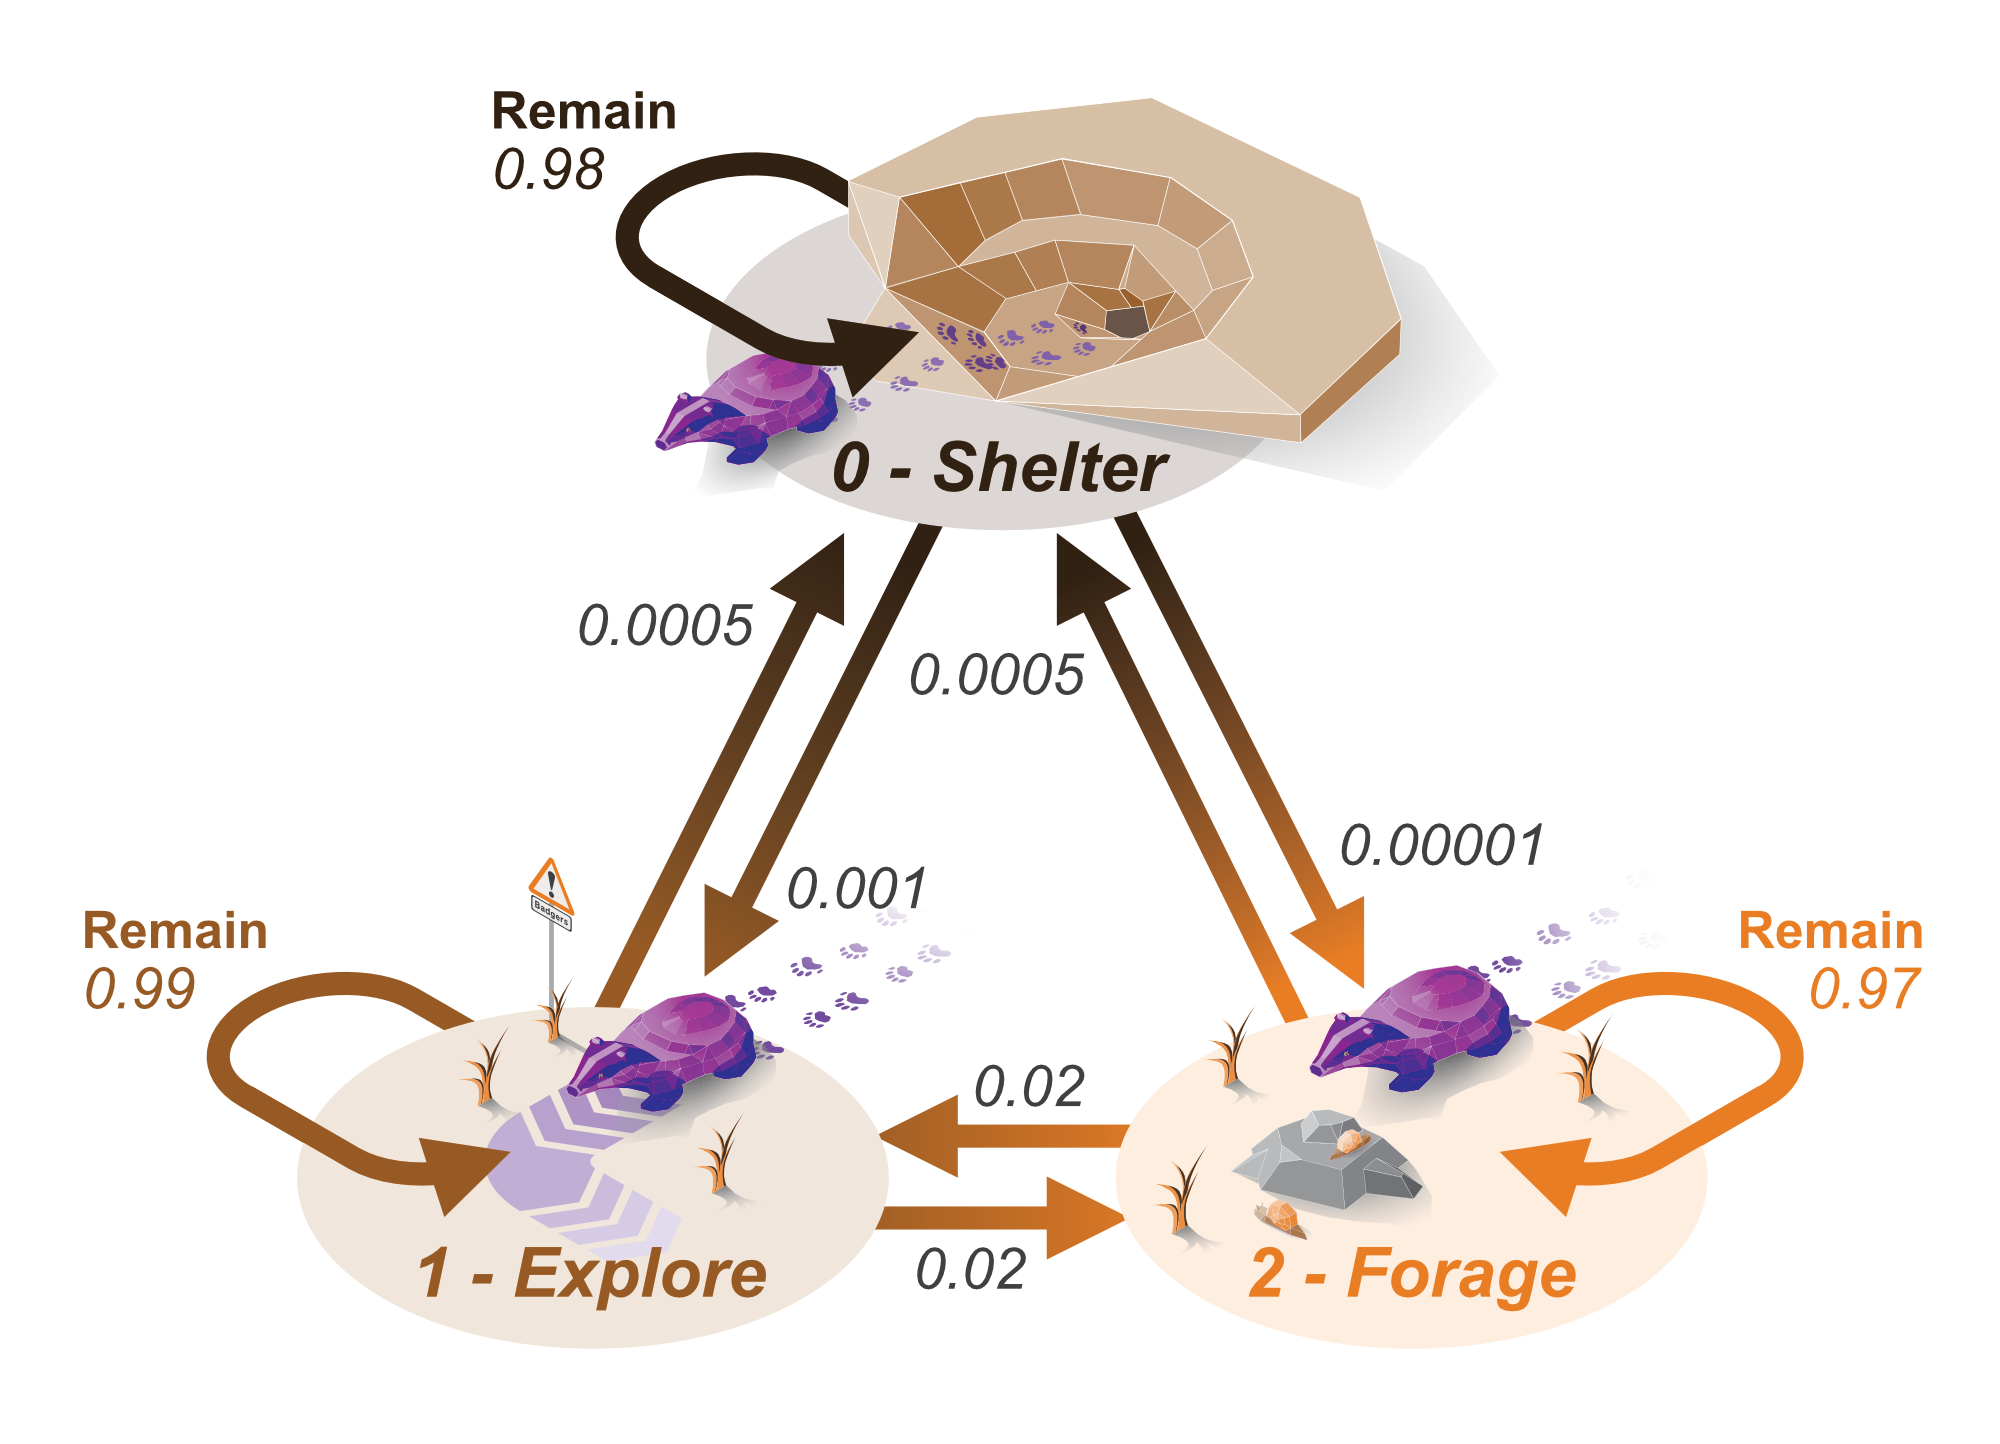
\includegraphics[width=0.8\linewidth]{../ext_figures/Tranistion Matrix Diagram} 

}

\caption{A diagram showing the simulated animal's decision processes operating at two different time frames. A - the time frame of the destination choice, B - the time frame of movements at each time step.}\label{fig:transMatrixDiagram}
\end{figure}

\begin{verbatim}
##      [,1]  [,2]    [,3]
## b0 0.9800 0.001 0.00001
## b1 0.0005 0.990 0.02000
## b2 0.0005 0.020 0.97000
\end{verbatim}

Animals behaviour is frequently expressed via cycles, such as day/night or diel cycles; therefore, we want the transition matrix vary over time.
We describe a number of cycles (or waves) that can be applied to the core transition matrix impacting the probability of entering resting behaviour.
We can define as many cycles as needed, and they impact the resting probability additively.

When entering the resting state the animal will seek out a shelter site.
In the \emph{abmAnimalMovement} package, we can supply a number of shelter sites to simulate this need and create site fidelity.
As these shelter sites at as points of attraction for the animal for each rest, the animal occupies a consistent area, or something approximating a home range.
Home ranges are mean to represent areas in which the animal can source all resources required for a given life stage.
The predefined and steady state of these shelter sites provides the stability we look for in a home range, as well as a means of predefining a level of site fidelity.
Using a point (or points) of attraction, is an approach that has reoccurred in movement and population ecology studies.
As the \emph{abmAnimalMovement} model can have multiple attraction (rest) sites supplied we can simulate home ranges with unequal and behavioural influenced space use.

\begin{figure}

{\centering 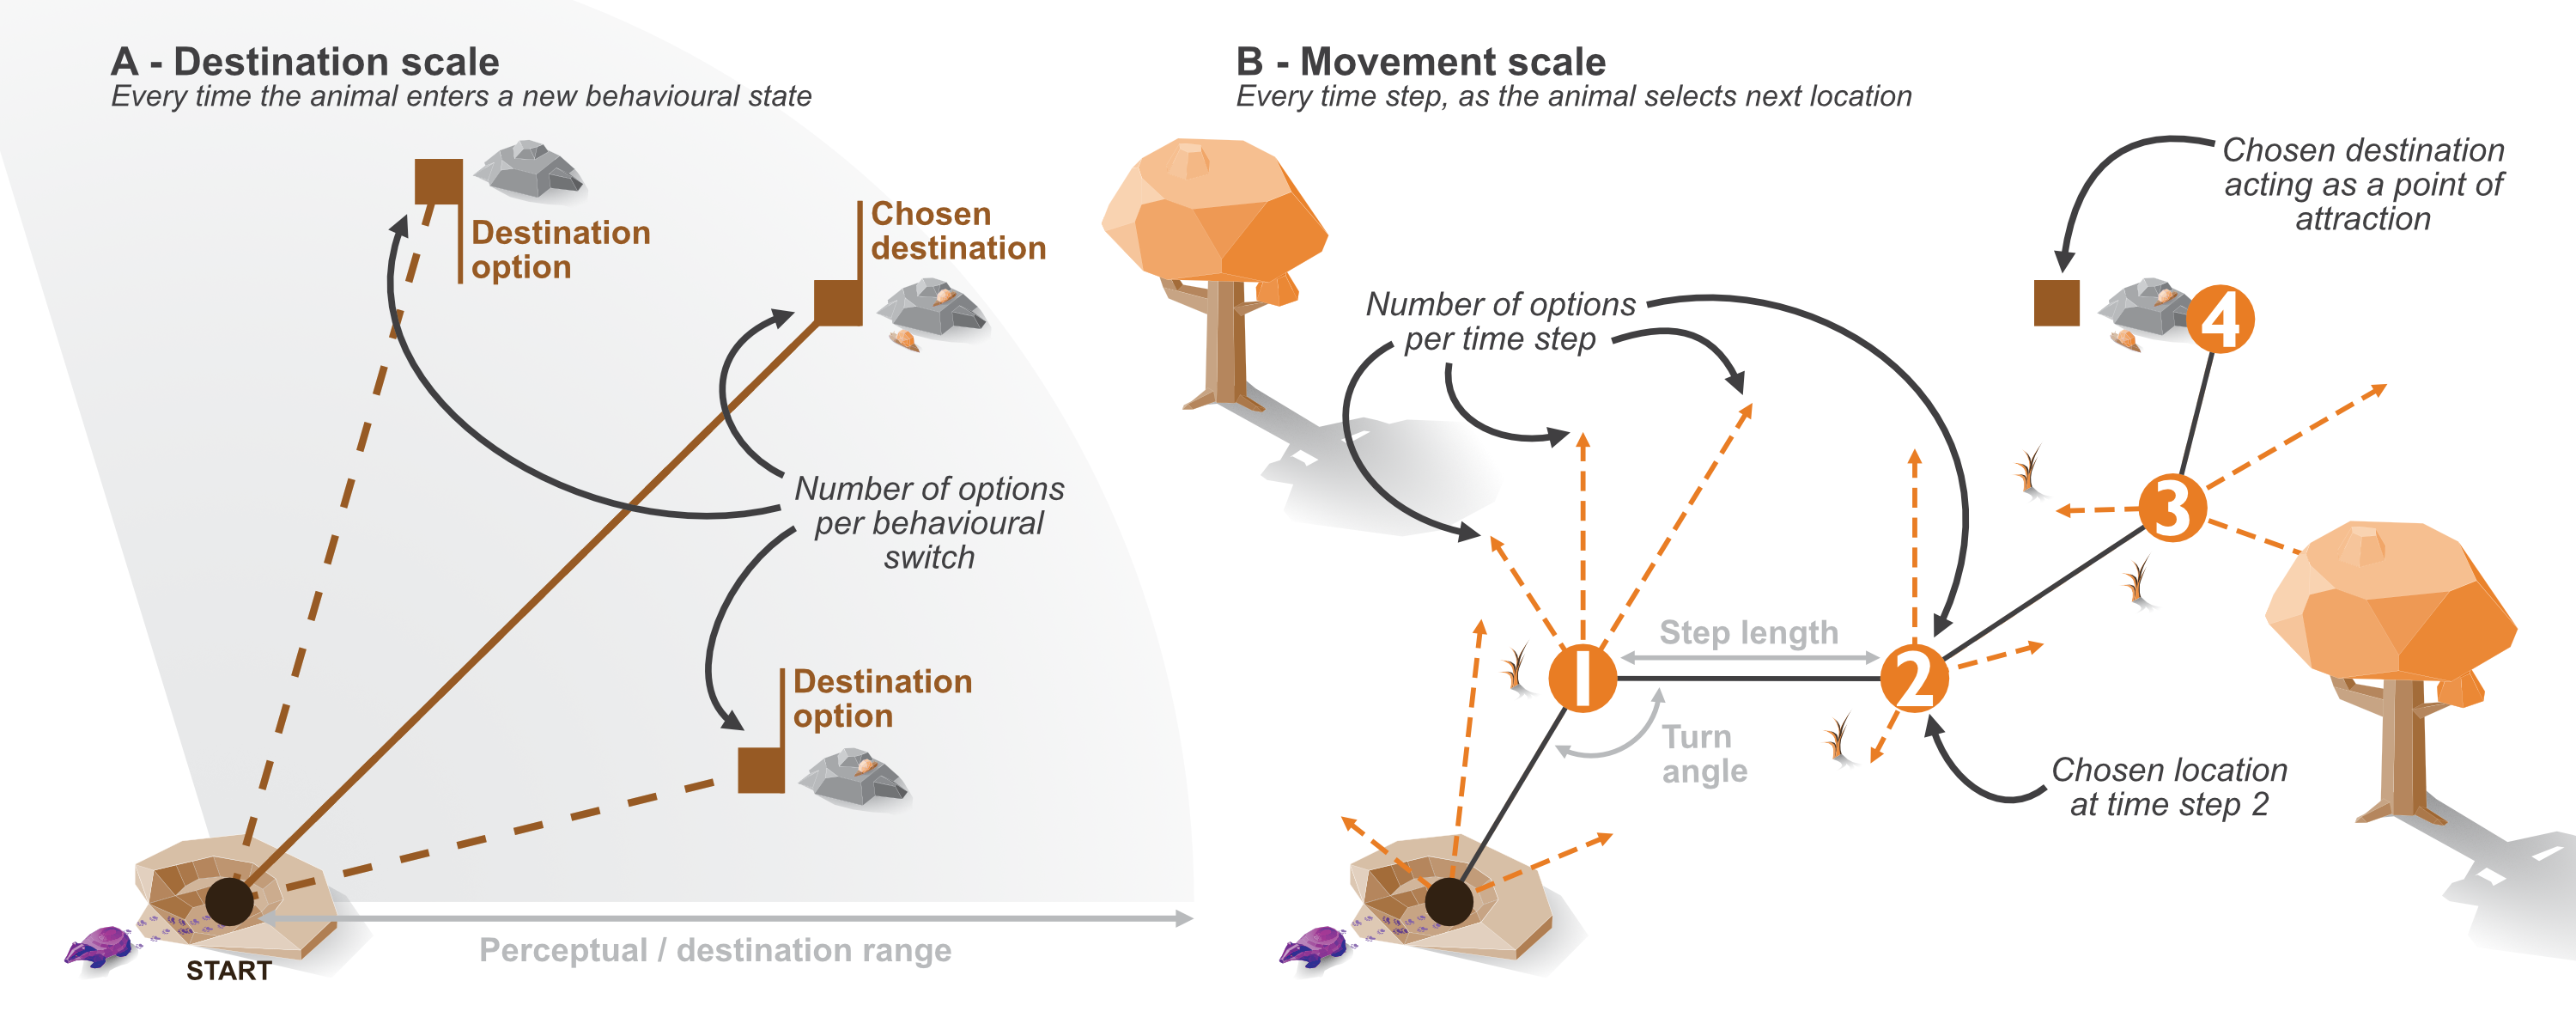
\includegraphics[width=0.8\linewidth]{../ext_figures/Simulation Process Diagram Static} 

}

\caption{A diagram showing the simulated animal's decision processes operating at two different time frames. A - the time frame of the destination choice, B - the time frame of movements at each time step.}\label{fig:walkDiagram}
\end{figure}

In addition to the predefined attraction to shelter sites, the \emph{abmAnimalMovement} package allows for a more dynamic attraction to areas of high resource quality.
As movements cannot be directly translated to animal preference; for example, habitat preference may miss key movement corridors (\protect\hyperlink{ref-Scharf2018}{49}); or the habitat decisions may occur at scales much broader to movement (\protect\hyperlink{ref-Bastille-Rousseau2017}{1}).
Therefore, the simulation required a mechanism that somewhat detaches the preference/choice for observed movements.
When entering foraging mode, the animal randomly selects (but weighted towards areas of higher quality) foraging destinations as a point of attraction {[}Figure \ref{fig:walkDiagram}{]}.
This attraction impacts the movement choices made at each time step, with the animal more likely to choose (and therefore move) options closer to the foraging destination.
Therefore, foraging destination choice operates on a different time frame to the movement and allows movements through low-quality foraging areas.
This presents a critical benefit of the simulation approach, as we define the internal state decision making process of the animal.
The two time frames also allows for explorations of assumptions connecting observed movement choices to choices regarding resources, and whether downstream analyses can accurately recover a hidden decision making process.

At all times the subsequent locations of the animal impacted by a movement resistance matrix.
Differing values represent different environmental conditions that could change how easily/likely an animal is to use that area to move towards a destination.
For example, rivers or hard barriers within a landscape could present very high movement resistance and a animal would aim to avoid traversing them.
Alternatively areas of lower movement resistance could aid movement, and potentially form movement corridors.
The movement matrix has values ranging from 0 to 1, that describes the movement probability.
Whereas the resource environmental layer and shelter locations interact with destination/goal decisions, the movement resistance affects the step-by-step movement decisions.

The interplay between shelter sites, foraging quality, and movement resistance simulates the site fidelity required for home ranges, while allowing the environment to help shape the size and diffusion of that home range.
Simulating a more dynamic and messy array of movements can help test how far assumptions of uniform circular animal movement are useful.

\hypertarget{generating-three-species}{%
\subsection{Generating Three Species}\label{generating-three-species}}

The best way to demonstrate the variation that movement ecology methods needs to wrangle, as well as the scope of movements the agent-based model can recreate, we provide three example species.
The examples cover a range of movement capacities, site fidelity, and resting/sheltering patterns.
None of the created examples are meant to directly match previously collected data on the species movements --there are alternative methods built to fit and simulate movements from existing data-- instead the examples provide some biological context to demonstrate a range of simulation parametrisations.
We split these examples into a more detailed walk-through, and two whose parametrisations are included in the supplementary materials.

\hypertarget{primary-example}{%
\subsection{Primary Example}\label{primary-example}}

\hypertarget{ecology-and-objectives---badger}{%
\subsubsection{Ecology and Objectives - Badger}\label{ecology-and-objectives---badger}}

Our primary example is based on a badger.
Badger occupy setts, in our example a two home/shelter sites, that they routinely return to (\protect\hyperlink{ref-kowalczyk_daily_2006}{50},\protect\hyperlink{ref-feore_habitat_1999}{51}).
When not at the sett the badger forages, and the foraging distances are impacted by resource position and movement capacity of the badger (i.e., how far can a badger feasibly travel for food from the sett).
The badger therefore expresses very high site fidelity, a range dictated by the spatial positioning of resources, and is subject to the movement resistance of the terrestrial environment.

We can draw on studies such as (\protect\hyperlink{ref-kowalczyk_daily_2006}{50}) and (\protect\hyperlink{ref-rosalino_activity_2005}{52}) to roughly gauge the speed of badgers (i.e., step length per minute).
How this speed differs between behaviours we more freely define, but use (\protect\hyperlink{ref-kowalczyk_daily_2006}{50}) reported maximum speed to guide more direct movements (e.g., state 0 and 1).
In particular (\protect\hyperlink{ref-kowalczyk_daily_2006}{50}) mentioned the heightened speeds moving from and to the setts.
We also want to allow the exploratory (state 1) movements to be great enough to occasionally exceed the normal home range or territory (\protect\hyperlink{ref-kelly_extra_2020}{53}).
We can draw on statements regarding maximum distance travelled in a night from papers such as (\protect\hyperlink{ref-rosalino_activity_2005}{52}), (\protect\hyperlink{ref-kowalczyk_daily_2006}{50}), and (\protect\hyperlink{ref-loureiro_path_2007}{54}) to approximate how distance foraging locations could be from a sett.
While also confirming the nocturnal activity cycle for the badger.
For the example, we will consider badgers as fully nocturnal, and with active periods lasting for around 8 hours each night (\protect\hyperlink{ref-rosalino_activity_2005}{52},\protect\hyperlink{ref-magowan_dead-reckoning_2022}{55}).
The 8 hour active periods are not consistent throughout the year.
Badger occupying temperate areas are impacted by seasonal shifts that modify daylight hours and available resources (\protect\hyperlink{ref-rosalino_activity_2005}{52},\protect\hyperlink{ref-magowan_dead-reckoning_2022}{55}).
Badger movements are also impacted by their territoriality, avoiding areas occupied by other badger groups, but also displaying occasional extra-territorial movements (\protect\hyperlink{ref-feore_habitat_1999}{51},\protect\hyperlink{ref-kelly_extra_2020}{53}).
This suggests a general but not complete avoidance of areas.

We can broadly summarise the badger ecology we want to parametrise as follows:

\begin{enumerate}
\def\labelenumi{\arabic{enumi}.}
\item
  Exhibits site fidelity via the use of two shelter sites
\item
  Movement speed approximated by summary statistics from previous studies, while constrained by terrestrial environment and territoriality
\item
  A 8-12 hour activity cycle, that shifts over the year
\end{enumerate}

\hypertarget{secondary-examples}{%
\subsection{Secondary Examples}\label{secondary-examples}}

We also provide example implementation of a vulture and king cobra -like movements, the exact values used can be found in the supplementary material.

\hypertarget{ecology-and-objectives---vulture}{%
\subsubsection{Ecology and Objectives - Vulture}\label{ecology-and-objectives---vulture}}

Unlike badgers and other terrestrially moving animals, vultures can move great distances with minimal obstruction {[}Figure \ref{fig:VULTURElayersFigure}{]}.
Vultures can also move greater distances more rapidly (\protect\hyperlink{ref-hribsek_first_2021}{56}), resulting in a more variable and distribution of step lengths (\protect\hyperlink{ref-garcia-jimenez_drivers_2018}{57}--\protect\hyperlink{ref-subedi_spatial_2020}{59}) {[}Figure \ref{fig:VULTUREsettingMoveDesPlot}{]}.

Similar to badgers vultures exhibit significant site fidelity, re-using roosting and nesting sites (\protect\hyperlink{ref-bracis_revisitation_2018}{60}).
Such shelter sites could be predefined; for example, if shelter sites were known \emph{a priori} discovered via the capture and tagged of animals, which in the case of birds is more likely.

Vultures also offer an opportunity to demonstrate how the underlying resource availability impact the movements of animals.
In the case of vultures, their moments have been seen to follow carcass, creating starkly contrasting areas where vultures will and will not travel (\protect\hyperlink{ref-arrondo_invisible_2018}{61}) {[}Figure \ref{fig:VULTURElayersFigure}{]}.

Vultures have a very similar cycle pattern to the badgers (just inverted), one defined by a standard 12 hours of activity during the day, and 12 hours of increased resting behaviour during the night.
The importance of simulating such cycles is made clear by vultures studies demonstrating that day-night cycles can impact rates of location collection (\protect\hyperlink{ref-silva_seasonal_2017}{62}).
How the the animals' activity cycle and the probability of collected data interact could be key consideration for some research questions.
Again similar to badgers we would expect seasonal shifts in the form of an increase and decrease in activity depending on the time of year (\protect\hyperlink{ref-hribsek_first_2021}{56},\protect\hyperlink{ref-garcia-jimenez_drivers_2018}{57},\protect\hyperlink{ref-peshev_new_2021}{63}).

We can broadly summarise the vulture ecology we want to parametrise as follows:

\begin{enumerate}
\def\labelenumi{\arabic{enumi}.}
\item
  Medium site fidelity via the use of multiple roosting/resting sites
\item
  Movement speed approximated by summary statistics from previous studies, with minimal landscape derived resistance
\item
  A 8-12 hour activity cycle, that shifts over the year
\end{enumerate}

\hypertarget{ecology-and-objectives---king-cobra}{%
\subsubsection{Ecology and Objectives - King Cobra}\label{ecology-and-objectives---king-cobra}}

Whereas the previous two species have a very limited or single shelter sites, king cobras make use of a wider range of shelter sites distributed more widely over their home ranges (\protect\hyperlink{ref-Marshall2018}{64},\protect\hyperlink{ref-marshall_no_2020}{65}).
These sites can also be larger, comprising burrow systems or rock complexes.

What more dramatically sets king cobras, and other snakes, apart is a vastly differing rest-forage cycle.
While snakes still exhibit a diel cycle, the intermittent depredation of large prey items and the time required sheltering to digest large meals results in a second broader activity cycle operating over a more widely observed diel cycle (\protect\hyperlink{ref-marshall_no_2020}{65}--\protect\hyperlink{ref-Siers2018}{68}).
We can conceptualise this pattern as two additive cycles, one that will describe the daily activity cycle, and a second that describes the foraging and digestion cycle.
Seasonality also impacts king cobra activity.
As king cobras occupy tropical regions, the seasonality they experience is not as pronounced as the badger or vulture examples.
Overall king cobras have three activity cycles acting on three different scales.

In this example we can also demonstrate the movement resistance dramatically impacting movement possibilities.
King cobra movement can be limited by roads (\protect\hyperlink{ref-jones_how_2022}{69},\protect\hyperlink{ref-Marshall2018b}{70}), where unless provided with crossing structures king cobras are vulnerable to vehicle hits {[}Figure \ref{fig:KINGCOBRAlayersFigure}{]}.
In addition to roads presenting linear barriers across the landscape, king cobras face persecution when near or in human settlements (\protect\hyperlink{ref-Marshall2018b}{70},\protect\hyperlink{ref-Shankar2013}{71}).
Despite the risks, avoidance of such areas appears weak.

Finally, king cobra movement characteristics will be dramatically reduced compared to the vulture's, but with similar shape to the badger with greater variability {[}Figure \ref{fig:KINGCOBRAsettingMoveDesPlot}{]} as king cobras are known to range over large areas (\protect\hyperlink{ref-Marshall2018}{64},\protect\hyperlink{ref-marshall_no_2020}{65},\protect\hyperlink{ref-Silva2018}{72}).

We can broadly summarise the king cobra ecology we want to parametrise as follows:

\begin{enumerate}
\def\labelenumi{\arabic{enumi}.}
\item
  Lower site fidelity via the use of many shelter sites
\item
  Movement speed approximated by summary statistics from previous studies, with examples of very high landscape derived resistance
\item
  A 8-12 hour activity cycle, with a approximately weekly forage-digest cycle, and weak seasonality
\end{enumerate}

\hypertarget{implementation}{%
\subsection{Implementation}\label{implementation}}

\hypertarget{required-libraries}{%
\subsubsection{Required Libraries}\label{required-libraries}}

First step is to load some libraries that will help us organise and visualise the inputs and outputs of the simulation.
Only the \emph{abmAnimalMovement} package is required for running the core simulation.

\begin{Shaded}
\begin{Highlighting}[]
\CommentTok{\# core package}
\FunctionTok{library}\NormalTok{(abmAnimalMovement)}
\CommentTok{\# data manipulation}
\FunctionTok{library}\NormalTok{(dplyr)}
\FunctionTok{library}\NormalTok{(reshape2)}
\CommentTok{\# visualisation}
\FunctionTok{library}\NormalTok{(ggplot2)}
\FunctionTok{library}\NormalTok{(ggforce)}
\FunctionTok{library}\NormalTok{(ggtext)}
\FunctionTok{library}\NormalTok{(ggridges)}
\FunctionTok{library}\NormalTok{(patchwork)}
\CommentTok{\# environmental matrix generation}
\FunctionTok{library}\NormalTok{(raster)}
\FunctionTok{library}\NormalTok{(NLMR)}
\end{Highlighting}
\end{Shaded}

We used \emph{R} v.4.2.1 (\protect\hyperlink{ref-R-base}{73}) via \emph{RStudio} v.2022.2.2.485 (\protect\hyperlink{ref-RStudioTeam2021}{74}), and made use \emph{rmarkdown} v.2.14 (\protect\hyperlink{ref-rmarkdown2020}{77}), \emph{bookdown} v.0.26 (\protect\hyperlink{ref-bookdown2016}{78},\protect\hyperlink{ref-R-bookdown}{79}), \emph{tinytex} v.0.39 (\protect\hyperlink{ref-tinytex2019}{80},\protect\hyperlink{ref-R-tinytex}{81}), and \emph{knitr} v.1.39 (\protect\hyperlink{ref-knitr2015}{82}--\protect\hyperlink{ref-R-knitr}{84}) packages to generate type-set outputs.
We the \emph{here} v.1.0.1 package (\protect\hyperlink{ref-R-here}{85}) to help with relative file path definition.
We used the \emph{dplyr} v.1.0.9 and \emph{reshape2} v.1.4.4 packages for data manipulation (\protect\hyperlink{ref-R-dplyr}{86},\protect\hyperlink{ref-reshape22007}{87}).
We used \emph{ggplot2} v.3.3.6 for creating figures (\protect\hyperlink{ref-R-ggplot2}{88},\protect\hyperlink{ref-ggplot22016}{89}), with the expansions: \emph{ggridges} v.0.5.3 (\protect\hyperlink{ref-R-ggridges}{90}), \emph{ggtext} v.0.1.1 (\protect\hyperlink{ref-R-ggtext}{91}), \emph{ggforce} v.0.3.3 (\protect\hyperlink{ref-R-ggforce}{92}), and \emph{patchwork} v.1.1.1 (\protect\hyperlink{ref-R-patchwork}{93}).
We used the \emph{raster} v.3.5.15 (\protect\hyperlink{ref-R-raster}{94}), \emph{sp} v.1.4.7 (\protect\hyperlink{ref-sp2013}{95}--\protect\hyperlink{ref-R-sp}{97}), and \emph{NLMR} v.1.1 (\protect\hyperlink{ref-NLMR2018}{98},\protect\hyperlink{ref-R-NLMR}{99}) for generating environmental matrices.

\hypertarget{generating-environmental-matrices}{%
\subsubsection{Generating Environmental Matrices}\label{generating-environmental-matrices}}

To ensure that the simulation completed during this example is repeatable, we set a seed.
For the sake of simplicity the year the examples was written --2022-- is used.

\begin{Shaded}
\begin{Highlighting}[]
\NormalTok{seed }\OtherTok{\textless{}{-}} \DecValTok{2022}
\FunctionTok{set.seed}\NormalTok{(seed)}
\end{Highlighting}
\end{Shaded}

Before starting to simulate animal movement we need to generate a landscape.
The landscapes in this case will take the form of matrices, where each cell is describing the quality of foraging, shelter, and movement ease.
The highest quality locations/cells are coded as 1, with quality decreasing as the values range down to 0.
The 1 to 0 quality values in each cell are later used to help the animal to chose how and where it moves throughout the landscape.
Depending on the behavioural state the weighing of which matrix/layer used will change (e.g., when in a resting behavioural state the shelter site quality layer is used).

For most applications a landscape would be known \emph{a priori}, but for this demonstration and testing of methods we will use a selection of random generated landscape matrices {[}Figure \ref{fig:BADGERlayersFigure}{]}.
To generate each layer (shelter, forage, movement) we use the \emph{NLMR} package (neutral landscape models), and combine a selection of landscape generation methods with \emph{landscapetools} (\protect\hyperlink{ref-Sciaini2018}{24}).

We used a Gaussian field with an autocorrelation range of 40, a magnitude of variation across the landscape of 5, magnitude of variation in the scale of autocorrelation range of 0.2, and a mean of 0.5.
For foraging, we build on the Gaussian field already produced, allocating all values lower than 0.4 as 0 (i.e., no value for foraging), then normalising the remaining values between 0 and 1.

For a baseline movement resistance layer, we take the original Gaussian field and increase areas greater than 0.6 by 0.5 to allow areas of high resource quality to be easily accessible.
We also greatly increase the movement ease in ``edge'' habitat (+1), where values fall between 0.6 and 0.3.
Again we normalise between 0 and 1, where 1 are areas easily traversed.
The resulting environment is one with easily traversable edge areas, surrounding better quality foraging locations than can be moved into easily.

Shelter quality is intermediate; we increased areas where cell values were greater than 0.3 and lower than 0.7.
Thereby shelter sites are more likely to occur in the areas of higher foraging quality, but not in the core (i.e., \textless0.7), nor in the edge areas (\textless0.5).
This provides some balance between accessibility and proximity to resources.
The three matrices described provide a baseline for our examples, but can easily be modified for different scenarios {[}Figure \ref{fig:BADGERlayersFigure}{]}.

\hypertarget{animal-parameters}{%
\subsubsection{Animal Parameters}\label{animal-parameters}}

We parametrise shelter information in the following ways.

For the sett, we draw a single set of coordinates (\texttt{shelterLocations}) from the shelter quality layer, and define the size of the shelter site as 8 m (\texttt{shelterSize}).
Shelter site size describes the distance from a shelter site that the animal dramatically lowers its movements; 8 m allows for small movements near/within the sett during resting behaviour.

\begin{Shaded}
\begin{Highlighting}[]
\NormalTok{sampledShelters }\OtherTok{\textless{}{-}} \FunctionTok{sampleRandom}\NormalTok{(}\FunctionTok{raster}\NormalTok{(landscapeLayersList}\SpecialCharTok{$}\NormalTok{shelter), }\DecValTok{2}\NormalTok{,}
                                \AttributeTok{ext =} \FunctionTok{extent}\NormalTok{(}\FloatTok{0.45}\NormalTok{, }\FloatTok{0.65}\NormalTok{, }\FloatTok{0.45}\NormalTok{, }\FloatTok{0.65}\NormalTok{),}
                                \AttributeTok{rowcol =} \ConstantTok{TRUE}\NormalTok{)}

\NormalTok{BADGER\_shelterLocs }\OtherTok{\textless{}{-}} \FunctionTok{data.frame}\NormalTok{(}
  \StringTok{"x"} \OtherTok{=}\NormalTok{ sampledShelters[,}\DecValTok{2}\NormalTok{],}
  \StringTok{"y"} \OtherTok{=}\NormalTok{ sampledShelters[,}\DecValTok{1}\NormalTok{])}

\NormalTok{BADGER\_shelterSize }\OtherTok{\textless{}{-}} \DecValTok{8}
\end{Highlighting}
\end{Shaded}

During the simulation the badger will randomly select a sett to return to, weighted by the values supplied via the shelter quality environmental layer {[}Figure \ref{fig:BADGERlayersFigure}{]}, each time it enters the resting behavioural state.

\begin{figure}

{\centering 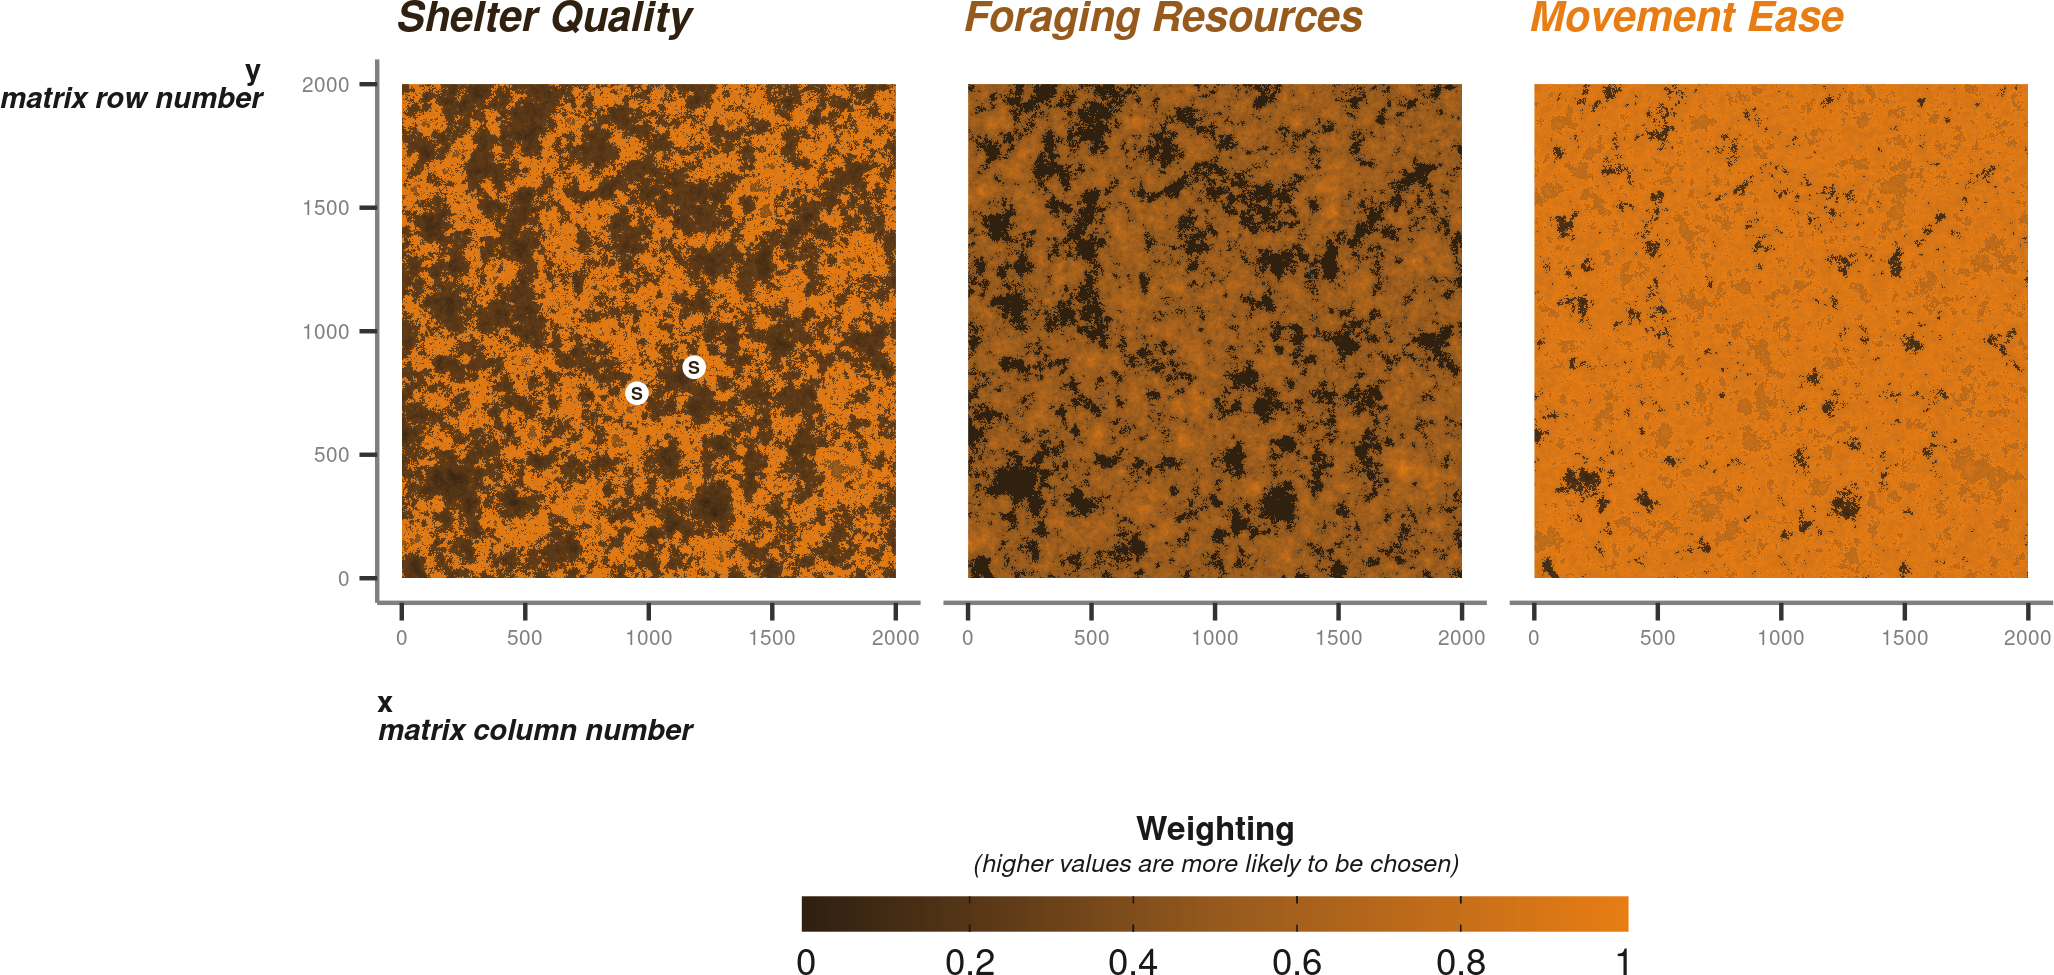
\includegraphics{Agent-based_model_walkthrough_files/figure-latex/BADGERlayersFigure-1} 

}

\caption{The three resulting landscape layers to be fed into the simulation for the badger example: shelter quality, foraging resources, movement ease.}\label{fig:BADGERlayersFigure}
\end{figure}

The movement of the badger is set via the definition of three pairs of Gamma and Von Misses distributions.
Each behavioural state is provided with a Gamma distribution to describe the step lengths between locations, and a Von Mises to describe the turn angles.
We provide these via \texttt{k\_step} and \texttt{s\_step} arguments for the shape (k) and scale (\(\theta\)) of the step Gamma distributions, as well as \texttt{mu\_angle} and \texttt{k\_angle} for the mean (\(\mu\)) and concentration (\(\kappa\)) of the Von Mises distribution.

The perceptual range, in other words, where the badger decides to forage is set in a similar fashion.
Where \texttt{destinationRange} provides the shape (k) and scale (\(\theta\)) for the Gamma distribution describing distance of foraging locations, and \texttt{destinationDirection} provides the mean (\(\mu\)) and concentration (\(\kappa\)) the Von Mises distribution describing the angle which those locations can fall {[}Figure \ref{fig:BADGERsettingMoveDesPlot}{]}.
We can also alter the strength of attraction to the foraging destinations with \texttt{destinationTransformation} and \texttt{destinationModifier}, where a stronger attraction will lead to more direct movements to the destinations chosen.

The rescale value is a simple means of adjusting the environment layers to fit with the scale/unit that the step lengths are provided in.
In this case we are treating each cell as a 5m by 5m, thereby ensuring that our 2000x2000 matrix is sufficient for the badger to traverse without leaving.
The rescale value therefore allows high resolution movements on lower resolution environments, offering a crucial memory saving optimisation.

\begin{Shaded}
\begin{Highlighting}[]
\NormalTok{BADGER\_k\_step }\OtherTok{\textless{}{-}} \FunctionTok{c}\NormalTok{(}\FloatTok{0.3}\SpecialCharTok{*}\DecValTok{60}\NormalTok{, }\FloatTok{1.25}\SpecialCharTok{*}\DecValTok{60}\NormalTok{, }\FloatTok{0.25}\SpecialCharTok{*}\DecValTok{60}\NormalTok{)}
\NormalTok{BADGER\_s\_step }\OtherTok{\textless{}{-}} \FunctionTok{c}\NormalTok{(}\FloatTok{0.8}\NormalTok{, }\FloatTok{0.25}\NormalTok{, }\FloatTok{0.5}\NormalTok{)}
\NormalTok{BADGER\_mu\_angle }\OtherTok{\textless{}{-}} \FunctionTok{c}\NormalTok{(}\DecValTok{0}\NormalTok{, }\DecValTok{0}\NormalTok{, }\DecValTok{0}\NormalTok{)}
\NormalTok{BADGER\_k\_angle }\OtherTok{\textless{}{-}} \FunctionTok{c}\NormalTok{(}\FloatTok{0.6}\NormalTok{, }\FloatTok{0.99}\NormalTok{, }\FloatTok{0.6}\NormalTok{)}

\NormalTok{BADGER\_destinationRange }\OtherTok{\textless{}{-}} \FunctionTok{c}\NormalTok{(}\DecValTok{3}\NormalTok{, }\DecValTok{120}\NormalTok{)}
\NormalTok{BADGER\_destinationDirection }\OtherTok{\textless{}{-}} \FunctionTok{c}\NormalTok{(}\DecValTok{0}\NormalTok{, }\FloatTok{0.01}\NormalTok{)}
\NormalTok{BADGER\_destinationTransformation }\OtherTok{\textless{}{-}} \DecValTok{2}
\NormalTok{BADGER\_destinationModifier }\OtherTok{\textless{}{-}} \DecValTok{2}

\NormalTok{BADGER\_rescale }\OtherTok{\textless{}{-}} \DecValTok{5}
\end{Highlighting}
\end{Shaded}

\begin{figure}

{\centering 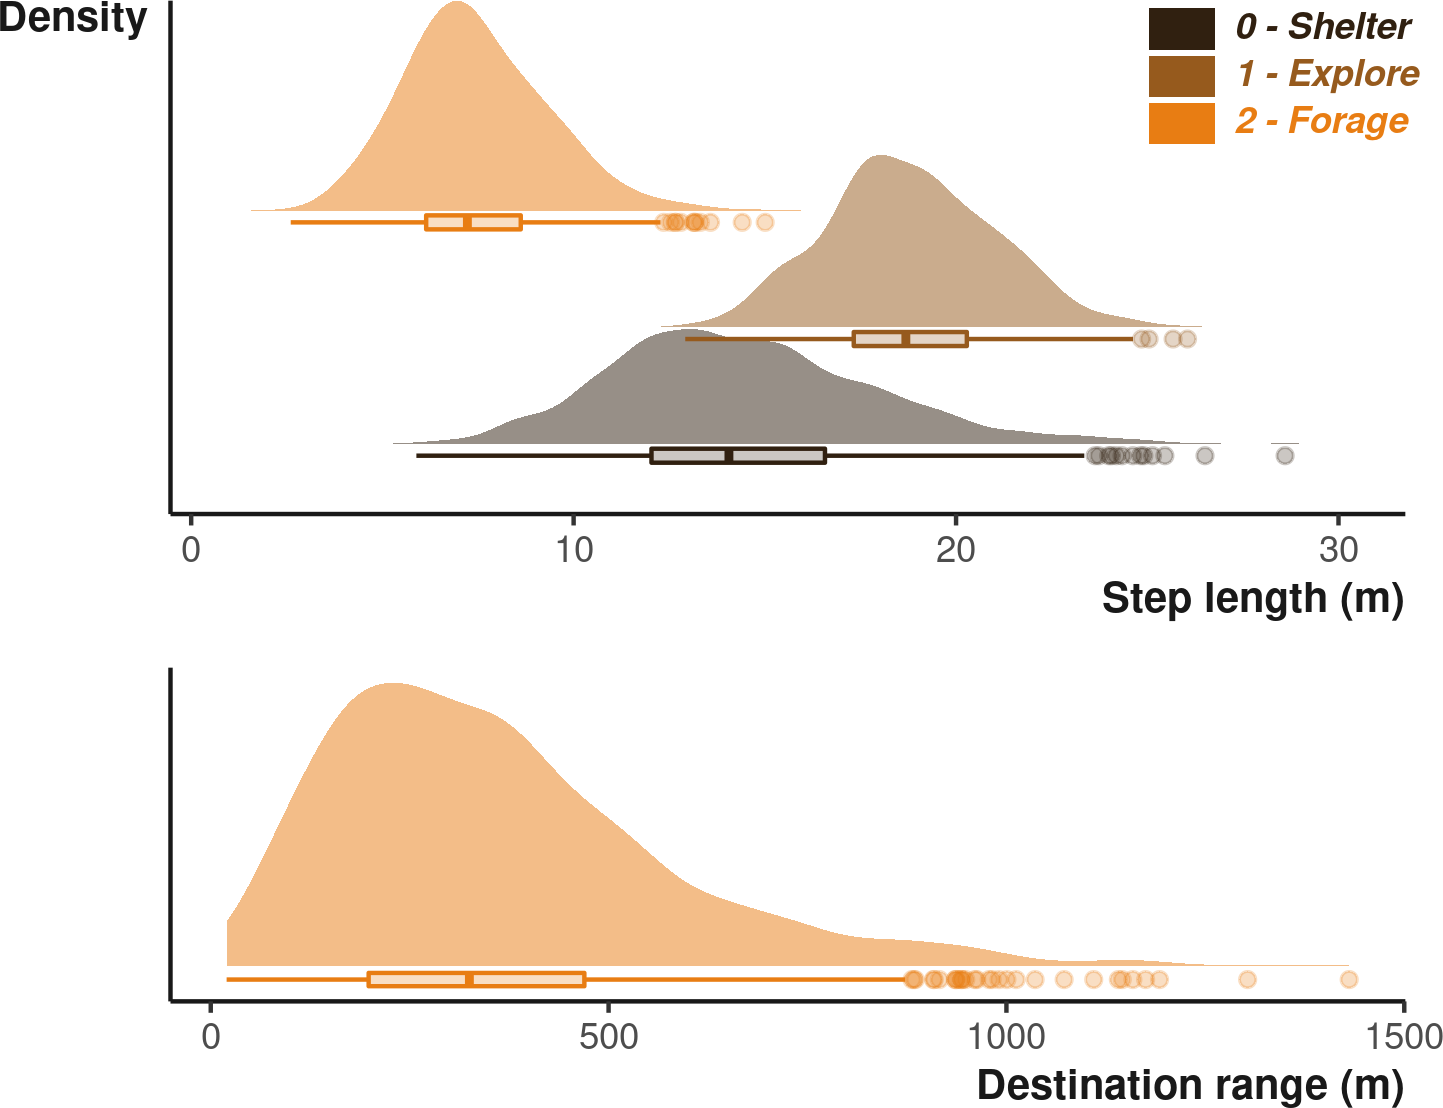
\includegraphics{Agent-based_model_walkthrough_files/figure-latex/BADGERsettingMoveDesPlot-1} 

}

\caption{The distribution of step lengths, and corresponding box plot for the badger example. The lower plot shows the distribution used to generate potential foraging desintations.}\label{fig:BADGERsettingMoveDesPlot}
\end{figure}

The territoriality is not simulated directly via other individuals, instead we approximate it by supplying a number of point locations the badger will avoid.
An alternative way of simulating this behaviour would be to create areas of high movement resistance prevent the badger from entering.
We provide a set of x, y coordinates of location to be avoided.
Alongside the locations we need to provide define how strongly the badger will avoid them using \texttt{avoidTransformation} and \texttt{avoidModifier.}
The avoidance behaviour will directly counteract the attraction to destination behaviour.

\begin{Shaded}
\begin{Highlighting}[]
\NormalTok{BADGER\_avoidLocs }\OtherTok{\textless{}{-}} \FunctionTok{data.frame}\NormalTok{(}
  \StringTok{"x"} \OtherTok{=} \FunctionTok{c}\NormalTok{(}\DecValTok{1205}\NormalTok{, }\DecValTok{1500}\NormalTok{, }\DecValTok{1165}\NormalTok{),}
  \StringTok{"y"} \OtherTok{=} \FunctionTok{c}\NormalTok{(}\DecValTok{980}\NormalTok{, }\DecValTok{1090}\NormalTok{, }\DecValTok{1250}\NormalTok{))}

\NormalTok{BADGER\_avoidTransformation }\OtherTok{\textless{}{-}} \DecValTok{2}
\NormalTok{BADGER\_avoidModifier }\OtherTok{\textless{}{-}} \DecValTok{4}
\end{Highlighting}
\end{Shaded}

We implement two cycles to capture the daily and seasonal cycles the badger experiences.
Both cycles are created by describing a wave defined by its amplitude, midline, offset (\(\phi\)) and frequency (\(\tau\)).
\texttt{rest\_Cycle} is a mandatory input geared toward diel activity cycling, and any number of additive additional cycles can be supplied using \texttt{additional\_Cycles}.
For our badger example, our 24 hour cycle modifies the probability of resting to result in rough 8 hour periods of activity.
This probability is modified by a seasonal wave increase the intensity of resting behaviour during a portion of the year, while not overwhelming a relatively stable diel cycle (i.e., badger will sleep longer during one part of the year).
A more extreme implementation of the second cycle could introduce hibernation behaviour.

\begin{Shaded}
\begin{Highlighting}[]
\NormalTok{BADGER\_rest\_Cycle }\OtherTok{\textless{}{-}} \FunctionTok{c}\NormalTok{(}\FloatTok{0.40}\NormalTok{, }\FloatTok{0.1}\NormalTok{, }\DecValTok{24}\NormalTok{, }\DecValTok{24}\NormalTok{)}

\CommentTok{\# additional cycle}
\NormalTok{c0 }\OtherTok{\textless{}{-}} \FunctionTok{c}\NormalTok{(}\FloatTok{0.2}\NormalTok{, }\DecValTok{0}\NormalTok{, }\DecValTok{24}\SpecialCharTok{*}\NormalTok{ (}\DecValTok{365}\SpecialCharTok{/}\DecValTok{2}\NormalTok{), }\DecValTok{24}\SpecialCharTok{*} \DecValTok{365}\NormalTok{) }\CommentTok{\# seasonal}

\NormalTok{BADGER\_additional\_Cycles }\OtherTok{\textless{}{-}} \FunctionTok{rbind}\NormalTok{(c0)}
\NormalTok{BADGER\_additional\_Cycles}
\end{Highlighting}
\end{Shaded}

\begin{verbatim}
##    [,1] [,2] [,3] [,4]
## c0  0.2    0 4380 8760
\end{verbatim}

\begin{Shaded}
\begin{Highlighting}[]
\NormalTok{BADGER\_behaveMatrix }\OtherTok{\textless{}{-}}\NormalTok{ Default\_behaveMatrix}
\NormalTok{BADGER\_behaveMatrix[}\DecValTok{1}\NormalTok{,}\DecValTok{1}\NormalTok{] }\OtherTok{\textless{}{-}} \FloatTok{0.95}
\NormalTok{BADGER\_behaveMatrix[}\DecValTok{1}\NormalTok{,}\DecValTok{2}\NormalTok{] }\OtherTok{\textless{}{-}} \FloatTok{0.005}
\NormalTok{BADGER\_behaveMatrix[}\DecValTok{1}\NormalTok{,}\DecValTok{3}\NormalTok{] }\OtherTok{\textless{}{-}} \FloatTok{0.005}
\NormalTok{BADGER\_behaveMatrix[}\DecValTok{2}\NormalTok{,}\DecValTok{3}\NormalTok{] }\OtherTok{\textless{}{-}} \FloatTok{0.01}
\NormalTok{BADGER\_behaveMatrix}
\end{Highlighting}
\end{Shaded}

\begin{verbatim}
##      [,1]  [,2]  [,3]
## b0 0.9500 0.005 0.005
## b1 0.0005 0.990 0.010
## b2 0.0005 0.020 0.970
\end{verbatim}

\hypertarget{running-the-simulation}{%
\subsubsection{Running the Simulation}\label{running-the-simulation}}

We need to initially define a start location for our animal.
To introduce some more individual variation we can randomly vary this starting location, but we will restrict the start locations to be proximal to the centre of the environment.
For the simulation we need a vector of length 2, where the first value is the x location, the second is y.

\begin{Shaded}
\begin{Highlighting}[]
\NormalTok{startLocation }\OtherTok{\textless{}{-}} \FunctionTok{sample}\NormalTok{(}\DecValTok{900}\SpecialCharTok{:}\DecValTok{1100}\NormalTok{, }\DecValTok{2}\NormalTok{, }\AttributeTok{replace =} \ConstantTok{TRUE}\NormalTok{)}
\end{Highlighting}
\end{Shaded}

We finally have some parameters that describe the scope and intensity of the simulation.

\begin{itemize}
\tightlist
\item
  How many time steps are simulated? In our examples we are operating under the assumption that one time step is equal to one minute.
  \texttt{timesteps}
\item
  How many options is the animal provided when deciding on its next location?
  \texttt{options}
\item
  How many destinations will the animal be able to chose from when it enters behaviour state 1 (foraging)?
  \texttt{des\_options}
\end{itemize}

We can then call all our settings we decided on previously describing badger behaviour and movement to run the simulation.

\begin{Shaded}
\begin{Highlighting}[]
\NormalTok{simSteps }\OtherTok{\textless{}{-}} \DecValTok{24}\SpecialCharTok{*}\DecValTok{60} \SpecialCharTok{*}\DecValTok{365}

\NormalTok{simRes }\OtherTok{\textless{}{-}} \FunctionTok{abm\_simulate}\NormalTok{(}\AttributeTok{start =}\NormalTok{ startLocation,}
                       \AttributeTok{timesteps =}\NormalTok{ simSteps,}
                       \AttributeTok{des\_options =} \DecValTok{10}\NormalTok{,}
                       \AttributeTok{options =} \DecValTok{12}\NormalTok{,}
                       \AttributeTok{k\_step =}\NormalTok{ BADGER\_k\_step,}
                       \AttributeTok{s\_step =}\NormalTok{ BADGER\_s\_step,}
                       \AttributeTok{mu\_angle =}\NormalTok{ BADGER\_mu\_angle,}
                       \AttributeTok{k\_angle =}\NormalTok{ BADGER\_k\_angle,}
                       \AttributeTok{rescale\_step2cell =}\NormalTok{ BADGER\_rescale}
                       
                       \AttributeTok{shelterLocations =}\NormalTok{ BADGER\_shelterLocs,}
                       \AttributeTok{shelterSize =}\NormalTok{ BADGER\_shelterSize,}
                       \AttributeTok{avoidPoints =}\NormalTok{ BADGER\_avoid,}
                       
                       \AttributeTok{destinationRange =}\NormalTok{ BADGER\_destinationRange,}
                       \AttributeTok{destinationDirection =}\NormalTok{ BADGER\_destinationDirection,}
                       \AttributeTok{destinationTransformation =}\NormalTok{ BADGER\_destinationTransformation,}
                       \AttributeTok{destinationModifier =}\NormalTok{ BADGER\_destinationModifier,}
                       \AttributeTok{avoidTransformation =}\NormalTok{ BADGER\_avoidTransformation,}
                       \AttributeTok{avoidModifier =}\NormalTok{ BADGER\_avoidModifier,}
                       
                       \AttributeTok{behave\_Tmat =}\NormalTok{ behaveMatTest,}
                       
                       \AttributeTok{rest\_Cycle =}\NormalTok{ BADGER\_restData,}
                       \AttributeTok{additional\_Cycles =}\NormalTok{ BADGER\_cycleMat,}
                       
                       \AttributeTok{shelteringMatrix =}\NormalTok{ BADGER\_shelter,}
                       \AttributeTok{foragingMatrix =}\NormalTok{ BADGER\_forage,}
                       \AttributeTok{movementMatrix =}\NormalTok{ BADGER\_move)}
\end{Highlighting}
\end{Shaded}

\hypertarget{results}{%
\section{Results}\label{results}}

\hypertarget{output-format}{%
\subsection{Output Format}\label{output-format}}

The simulation function (\texttt{abm\_simulate}) outputs a list containing: a dataframe of realised movements, a dataframe of options the animal had available, and a list of the inputs used to simulate the movement.
The realised movement dataframe (\texttt{locations}) describes all realised locations the animal occupied, step length information, behavioural state, and current point of attraction, where each row is equal to a timestep.
Note the simulation is scale agnostic, so each row can represent a different timestep.
Other than the lack of a time stamp and location error the format largely mirrors a typical movement dataset.
Our example is minute by minute; changing the timestep would require a reparametrisation of step length and behavioural transition probabilities.
The \texttt{options} dataframe describes all the options available to the animal over the entire simulation duration, where each row is equal to an option repeated for each timestep.

\hypertarget{outputs-review}{%
\subsection{Outputs Review}\label{outputs-review}}

Once ran we can review the movement characteristics of the three species.
The simplest to examine is the movement speeds or step lengths.
During the simulation parametrisation we provided a rescale values to describe the the size of the cells describing environmental information (see \texttt{rescale\_step2cell} argument).
The simulated movement will return the scaled values, so to plot something comparable to the input values we must rescale the simulated step lengths.

\begin{figure}

{\centering 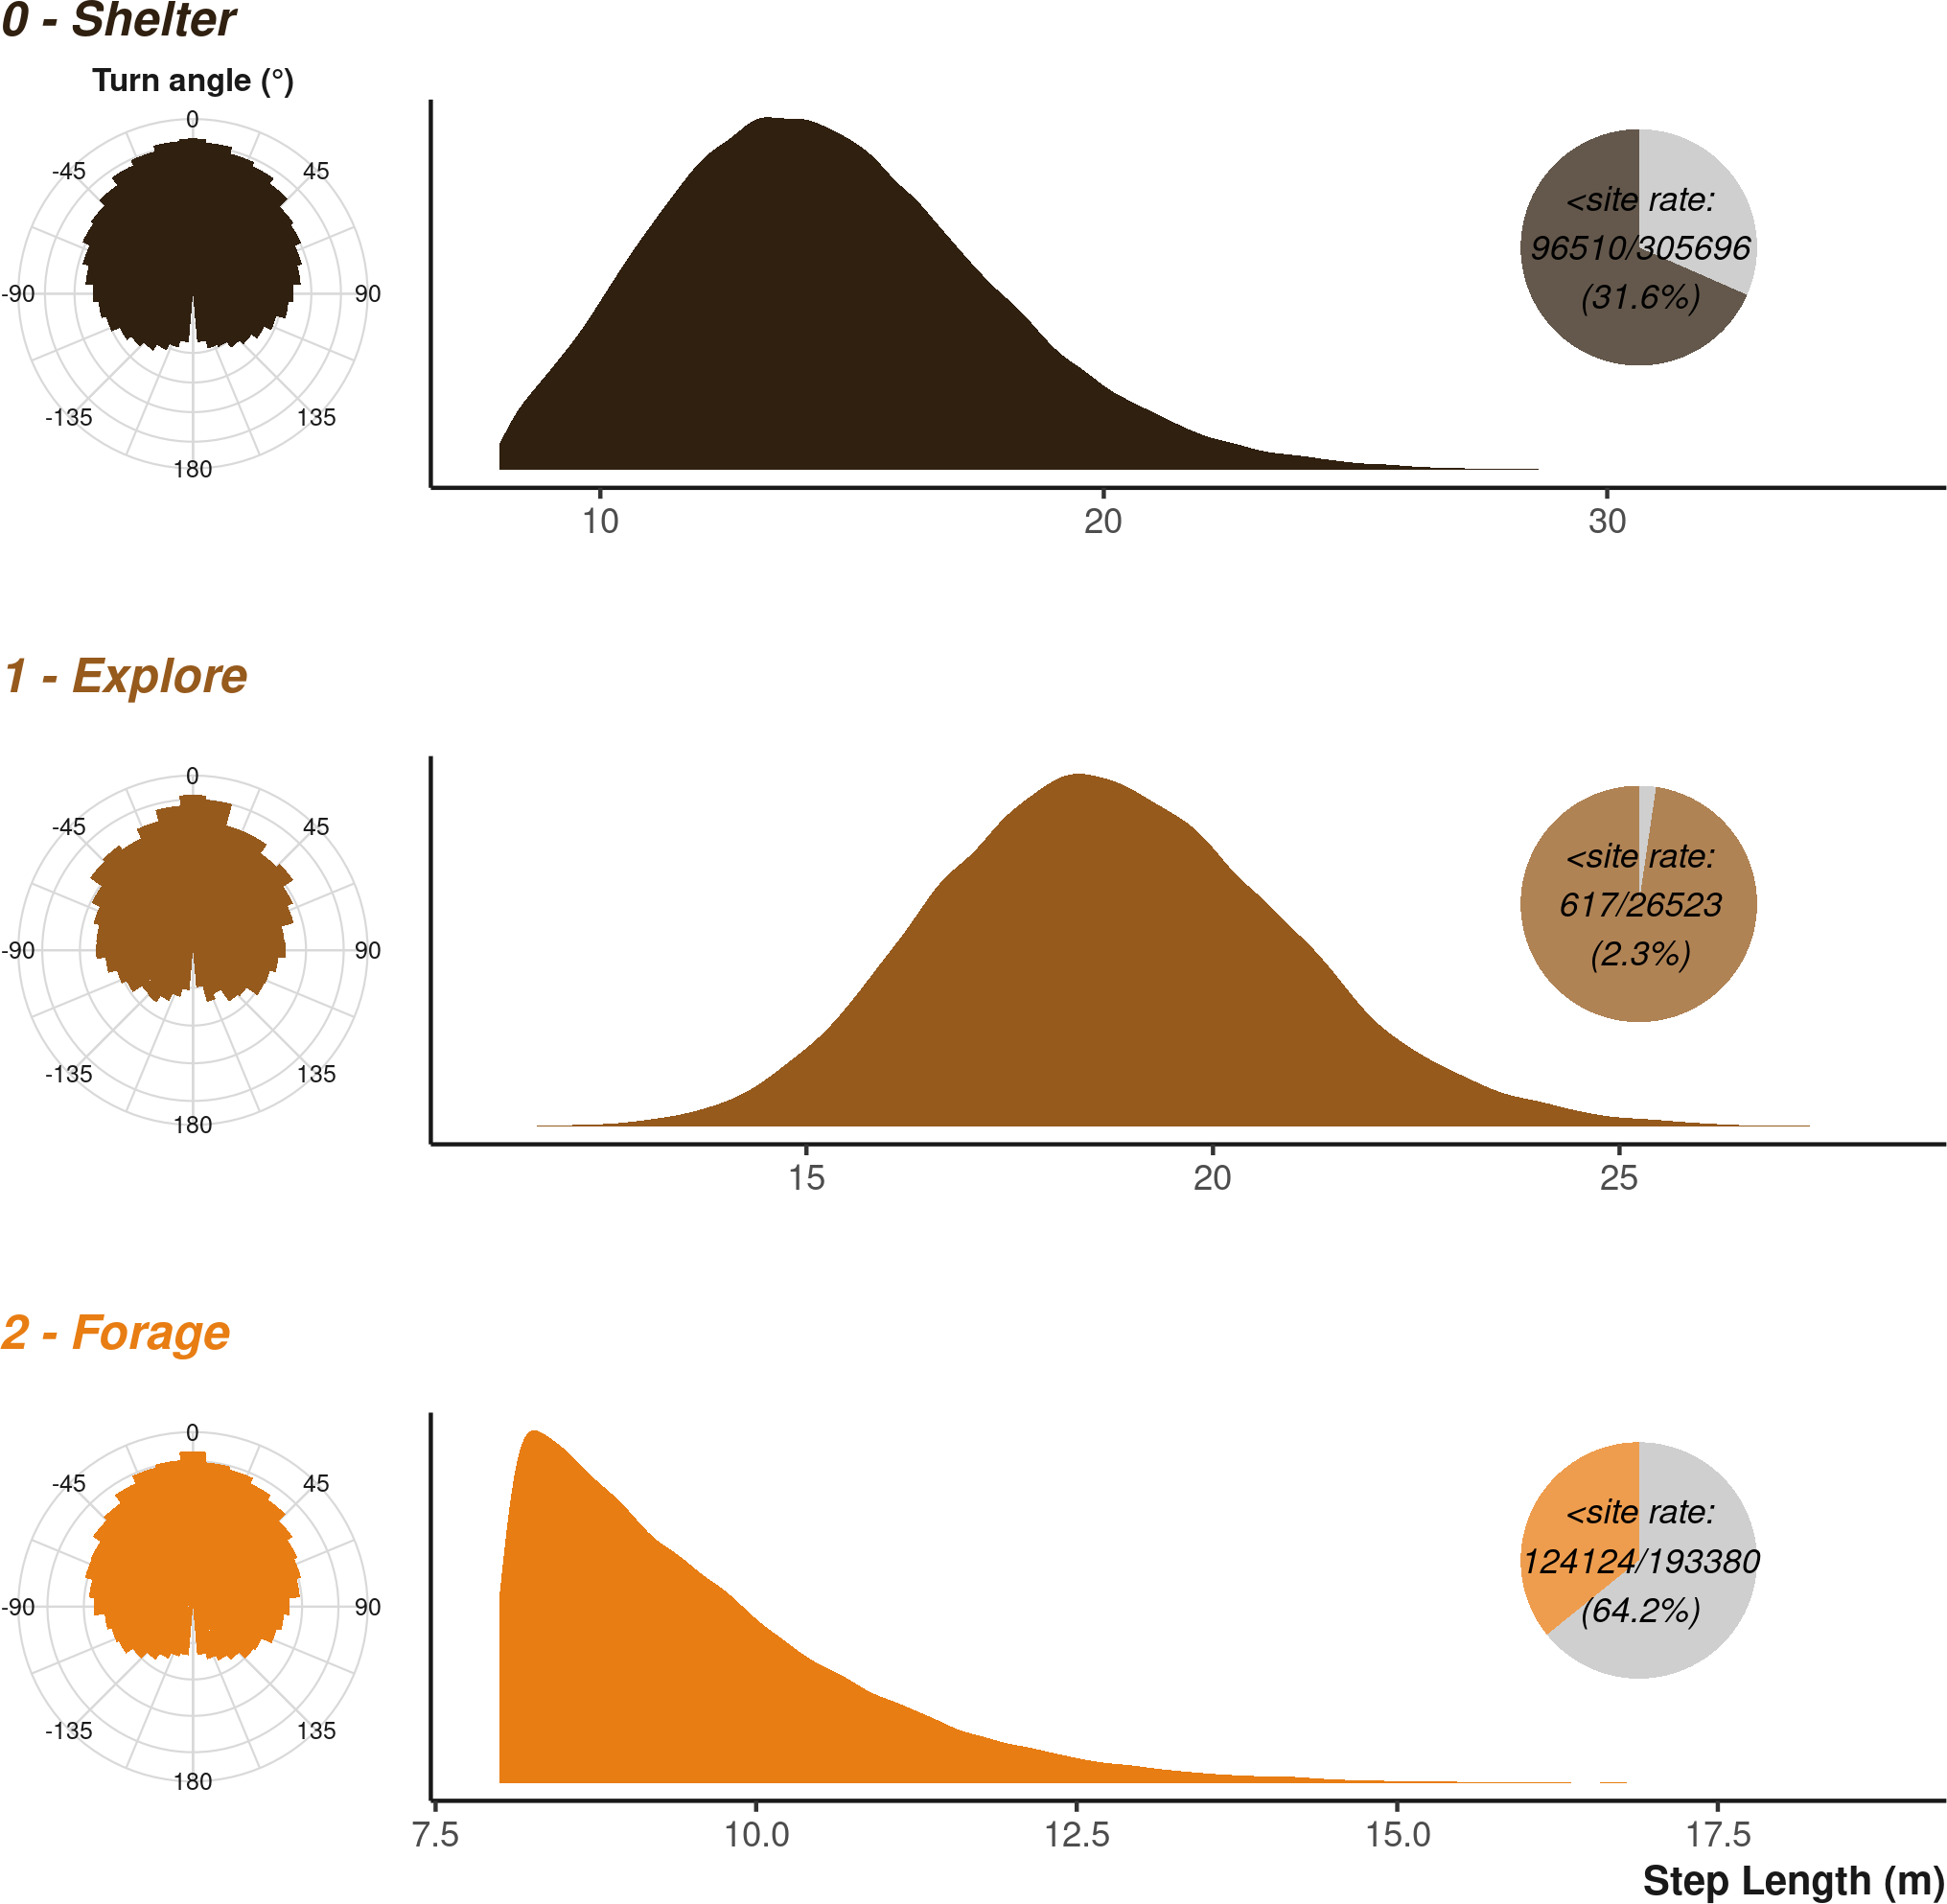
\includegraphics{Agent-based_model_walkthrough_files/figure-latex/BADGERmoveCharFigure-1} 

}

\caption{The badger example's observed turn angles and step lengths resulting from the simulation. Step lengths are scaled back to the input units. Inset pie chart show the number of step lengths that were below the shelter site size; the sub-shelter site step lengths are excluded from the density plot. Note that x axis is not consistent between the three plots.}\label{fig:BADGERmoveCharFigure}
\end{figure}

We can compare the inputs from Figure \ref{fig:BADGERsettingMoveDesPlot} to the observed outputs in Figure \ref{fig:BADGERmoveCharFigure} and see that they largely agree as expected.
The turn angles are more variable, as the destination decisions and attraction to locations heavily influence the distribution overriding the parametrisation of the Von Mises.
Figure \ref{fig:VULTUREsettingMoveDesPlot} and Figure \ref{fig:KINGCOBRAsettingMoveDesPlot} in the supplementary figure show the outputs for vulture and king cobra simulations.

We can review how the movements appear in space.
With the badger example the impact of the avoidance points is clearly visible {[}Figure \ref{fig:mapsFigure}a{]}, whereas the lack of or weaker avoidance in vulture {[}Figure \ref{fig:mapsFigure}b{]} and king cobra {[}Figure \ref{fig:mapsFigure}c{]} makes the avoidance less influential.
The vulture's movements and chosen foraging locations are largely to the east, demonstrating the impact of the underlying foraging quality environmental layer.
Foraging differences are also very apparent in the king cobra plot.
The highlighted sheltering behaviour means that the king cobra made fewer shifts to the foraging behaviour resulting in fewer dynamically selected foraging destinations.

\begin{figure}

{\centering 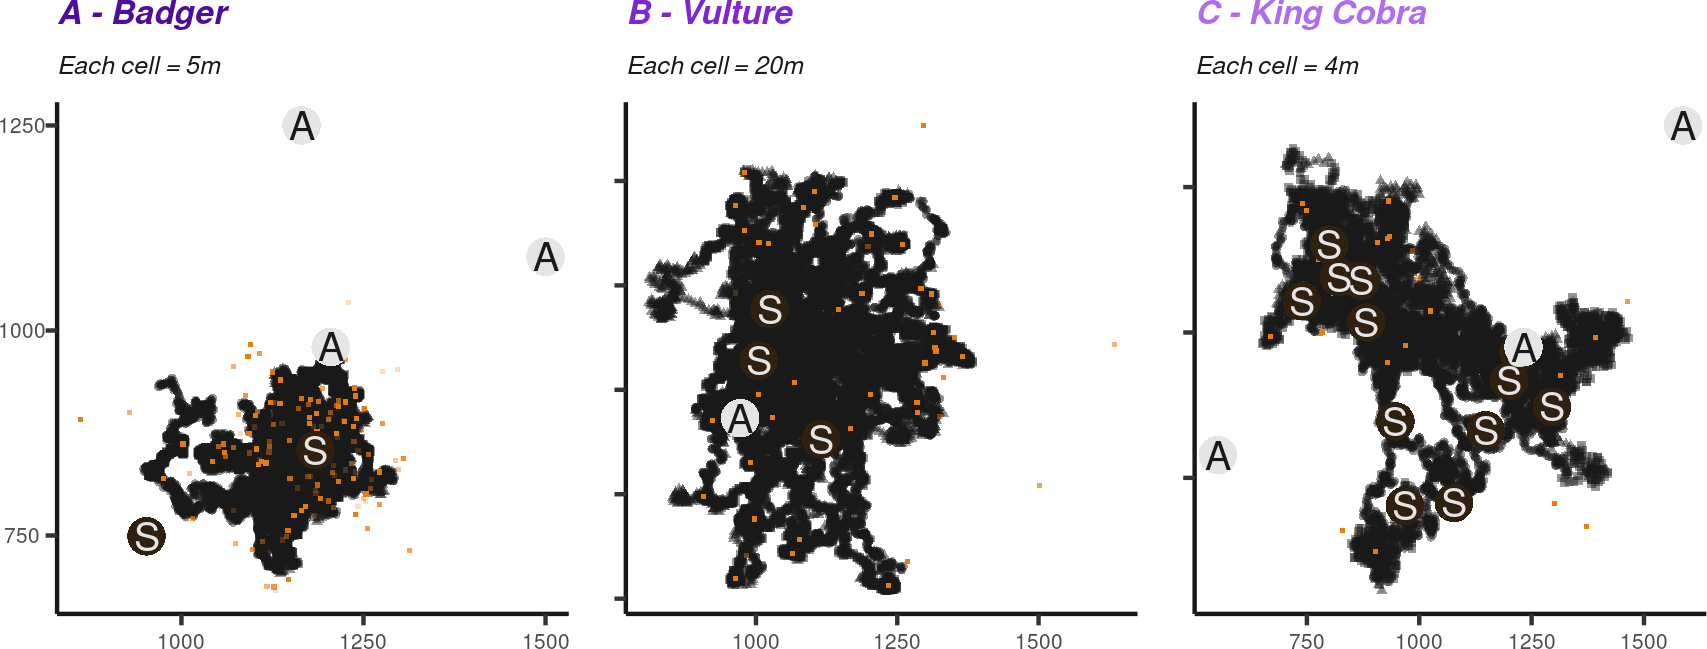
\includegraphics{Agent-based_model_walkthrough_files/figure-latex/mapsFigure-1} 

}

\caption{The observed locations of the three simulated species (A - Badger, B - Vulture, C - King Cobra). Black points show the observed location at each time step, with the current behavioural state (circle = shelter, triangle = explore, square = forage). The orange squares show the dynamically selected foraging destinations. Circles with an interior S show the shelter site locations, and cricles with an interior A show the avoidance points. Note that the size represented by each unit on the x and y axis differs depending on the species.}\label{fig:mapsFigure}
\end{figure}

\begin{figure}

{\centering 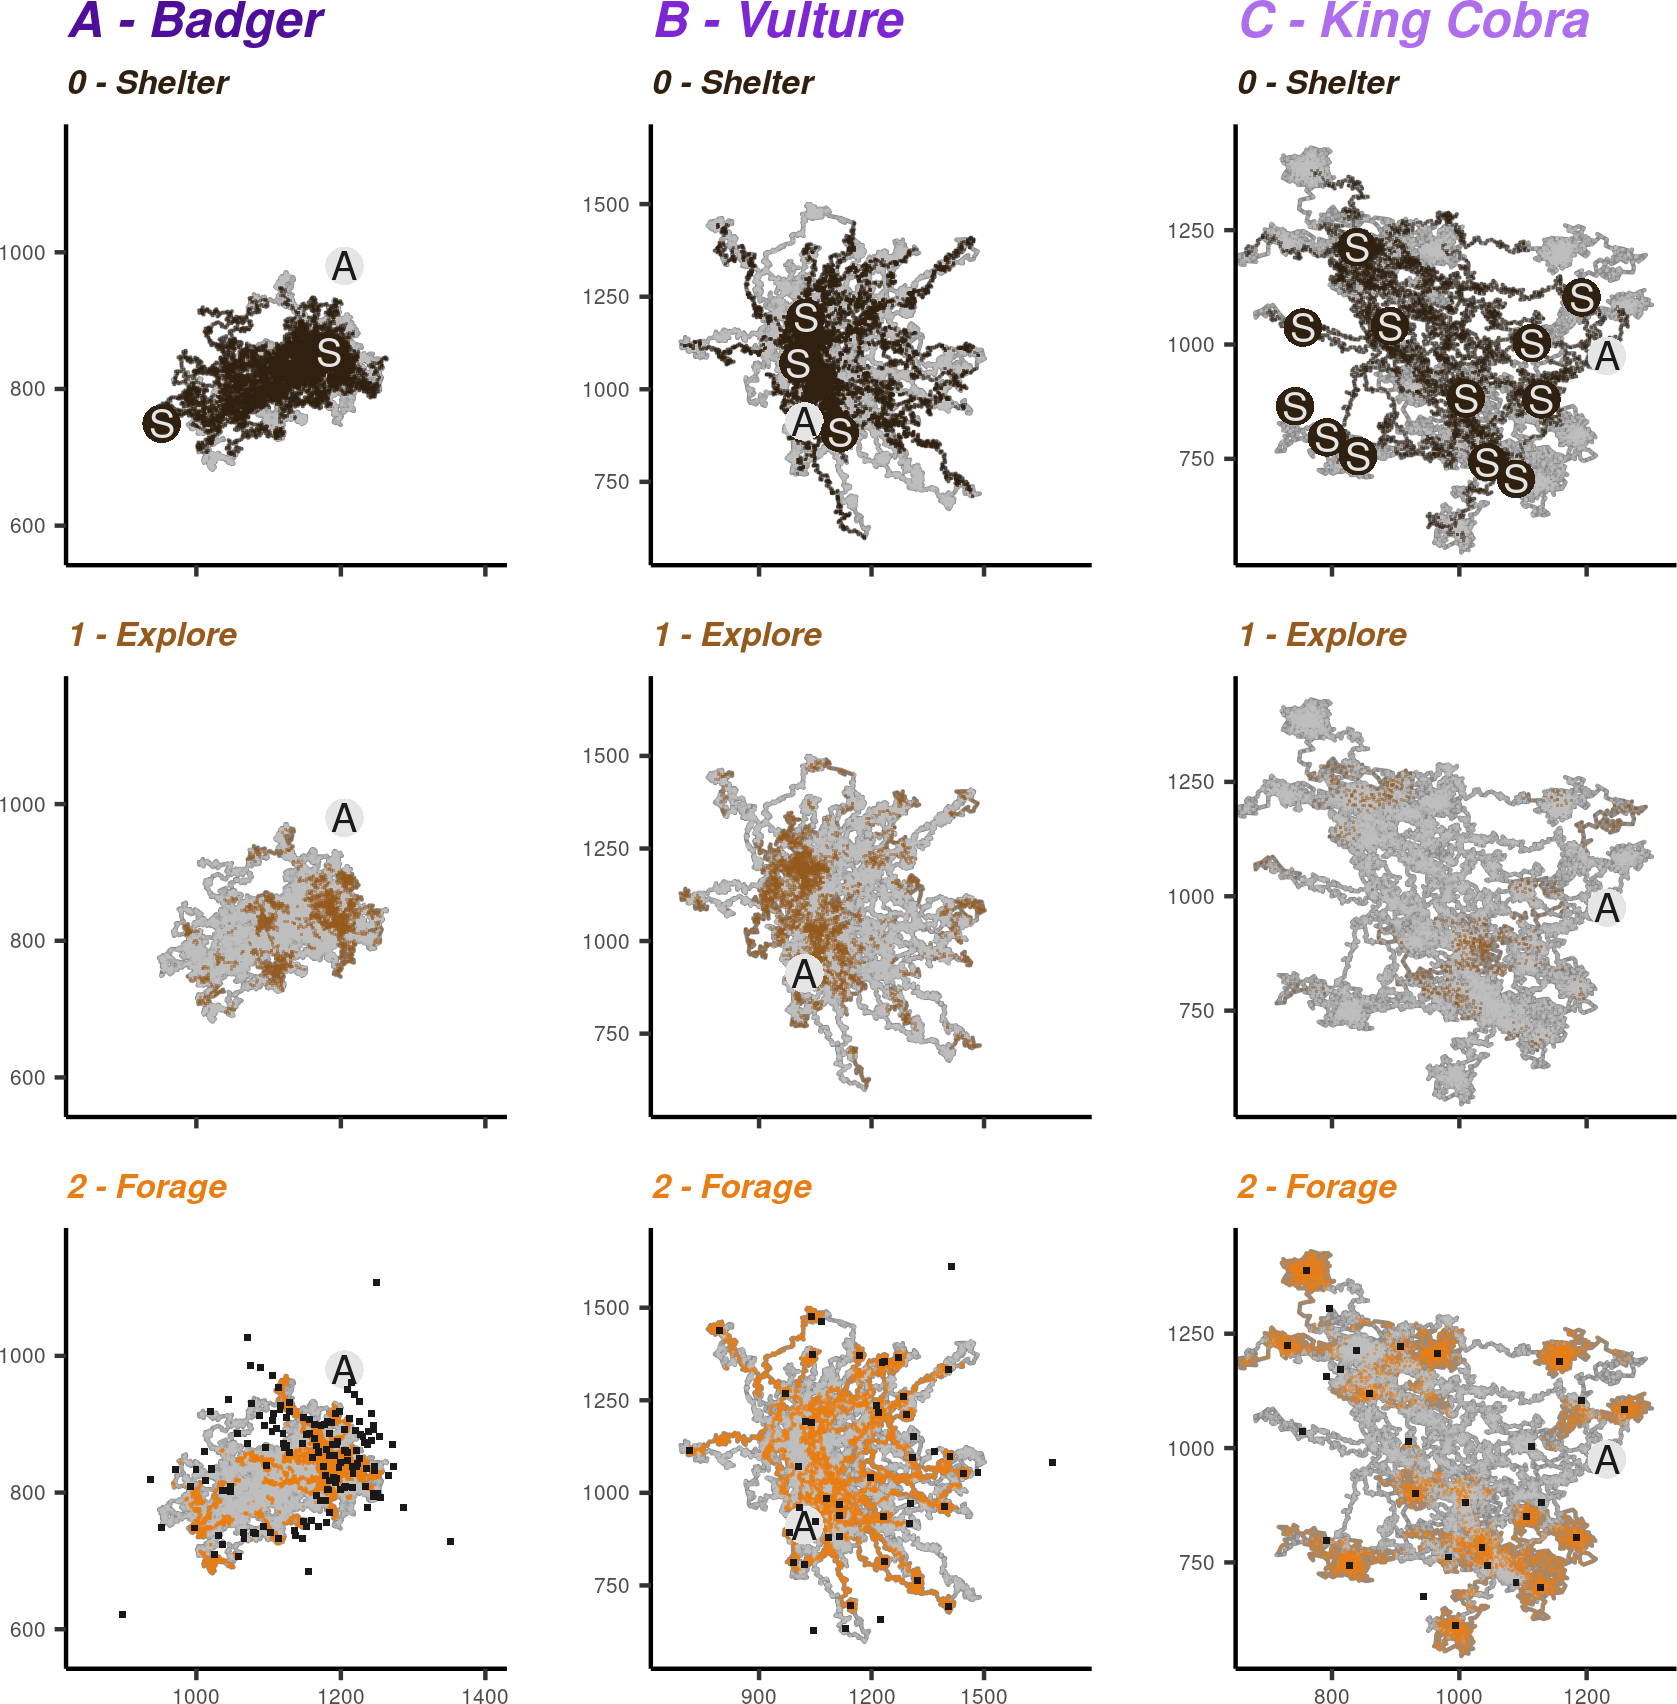
\includegraphics{Agent-based_model_walkthrough_files/figure-latex/oneMonthMapFigure-1} 

}

\caption{The observed locations of the three simulated species (A - Badger, B - Vulture, C - King Cobra) over the first month of time steps. Grey path shows the overall movement during that month, overlaid points indicate where the animal was in a given behavioural mode. Circles with an interior S show the shelter site locations, and cricles with an interior A show the avoidance points, black squares show the dynamically selected foraging destinations. Note that the size represented by each unit on the x and y axis differs depending on the species.}\label{fig:oneMonthMapFigure}
\end{figure}

The activity cycles and the timing of behavioural shifts is a key component in the simulations.
We can examine that the predefined cycles are resulting in expected patterns.
A year worth of data makes observing all but the broadest cycles difficult to visualise, so in Figure \ref{fig:cycleFigure} we can look at several months worth of day as well as the daily cycle.
Badger and vulture daily cycles are largely the same {[}Figure \ref{fig:cycleFigure}a \& b{]}, with a consistent daily activity cycle differing only slightly in the time spent active and balance between shifts from sheltering to foraging and exploring.
Some of the differences are a result of the different behavioural transition matrix provided to simulated the two species, where both had different baseline probabilities of shifting between behavioural states.
By contrast, the king cobra example demonstrates the interaction between the daily and weekly cycle we input {[}Figure \ref{fig:cycleFigure}{]}.
We can see we intermittently get extended sheltering periods, punctuated by short exploratory or foraging bouts.

\begin{figure}

{\centering 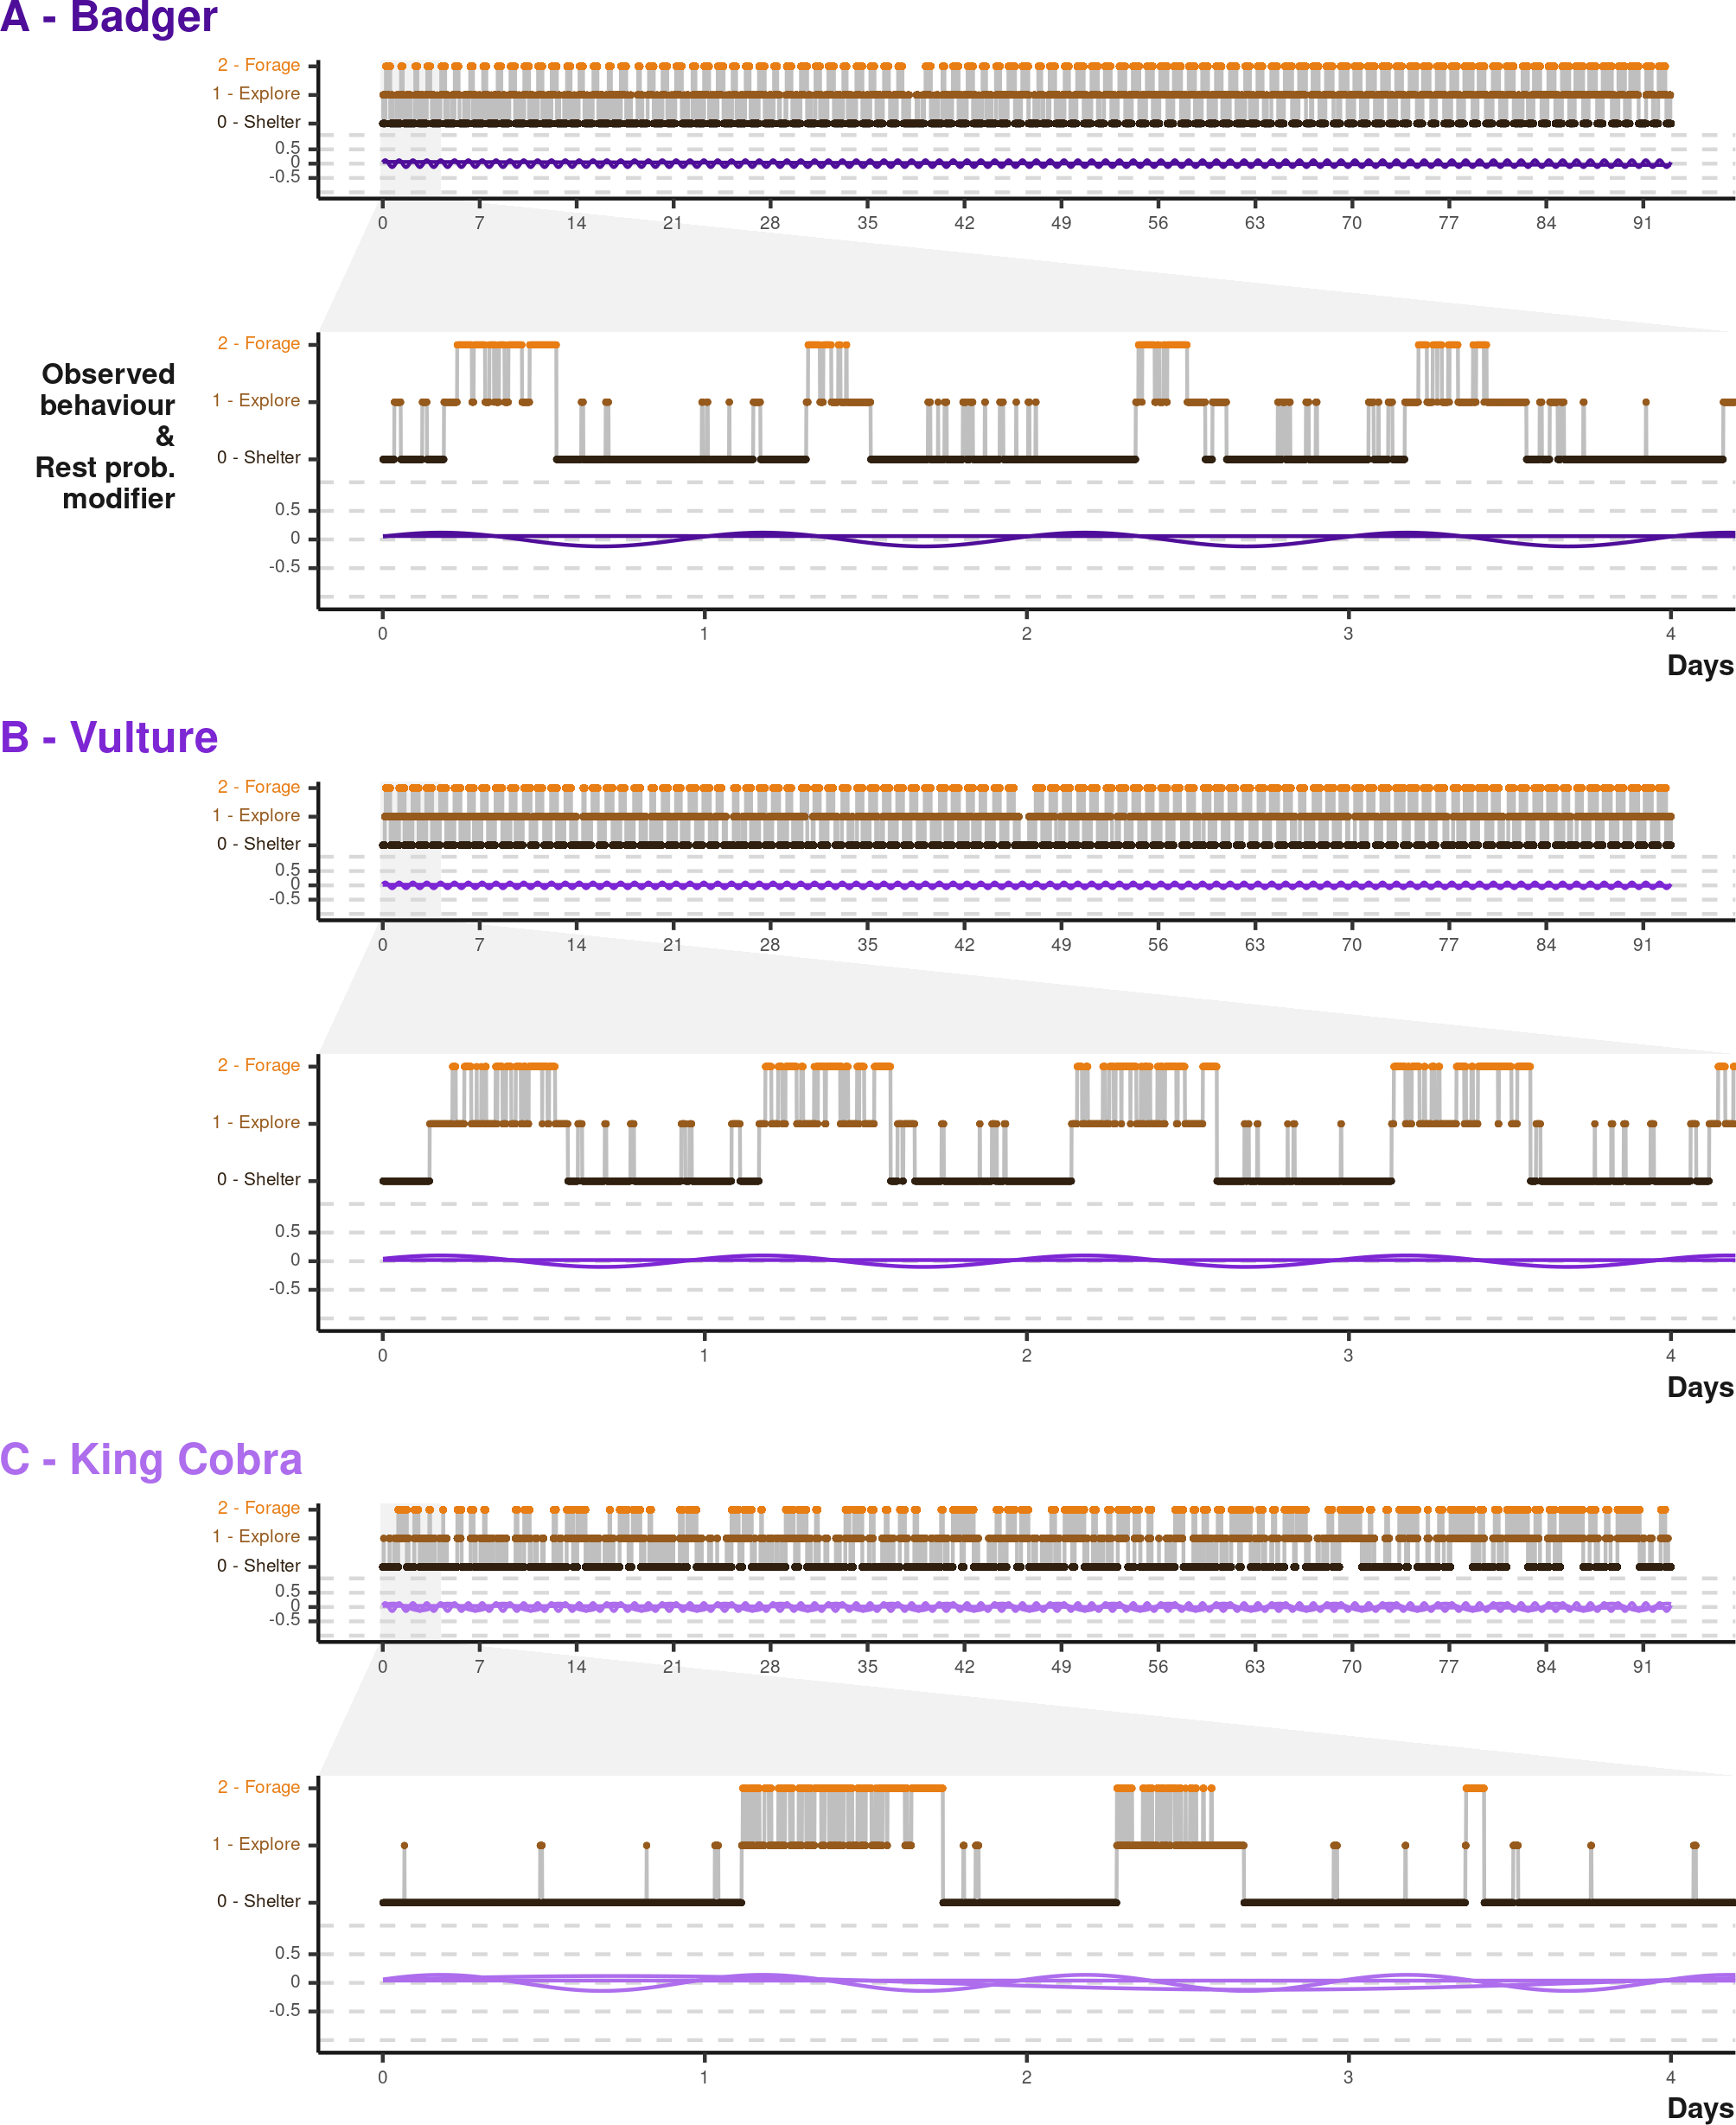
\includegraphics{Agent-based_model_walkthrough_files/figure-latex/cycleFigure-1} 

}

\caption{The observered (top half) and parametrised activty cycles (bottom half) governing sheltering behaviour in the three example species (A - Badger, B - Vulture, C - King Cobra). Point colour and position describe the behavioural state at each simulated time step, whereas the purple waves indicated the input values. Note that the input waves acting on the simulated animal in conjunction with the beahvioural transition matrix.}\label{fig:cycleFigure}
\end{figure}

At the daily and monthly scale we cannot see the impact of the broad scale seasonal cycles.
Instead we can look at the percentage of time steps per day the animal was in sheltering behaviour {[}Figure \ref{fig:cycleSeasonalFigure}{]}.
Again the Badger and Vulture sheltering rates are similar, differing in intensity, but with both demonstrating a seasonal decrease in the middle of the simulation.
The king cobra cycles reveals an decrease in the number of days spent entirely sheltering, and an overall impression that the seasonal cycle is less influential (as it is only one of three activity cycles).

\begin{figure}

{\centering 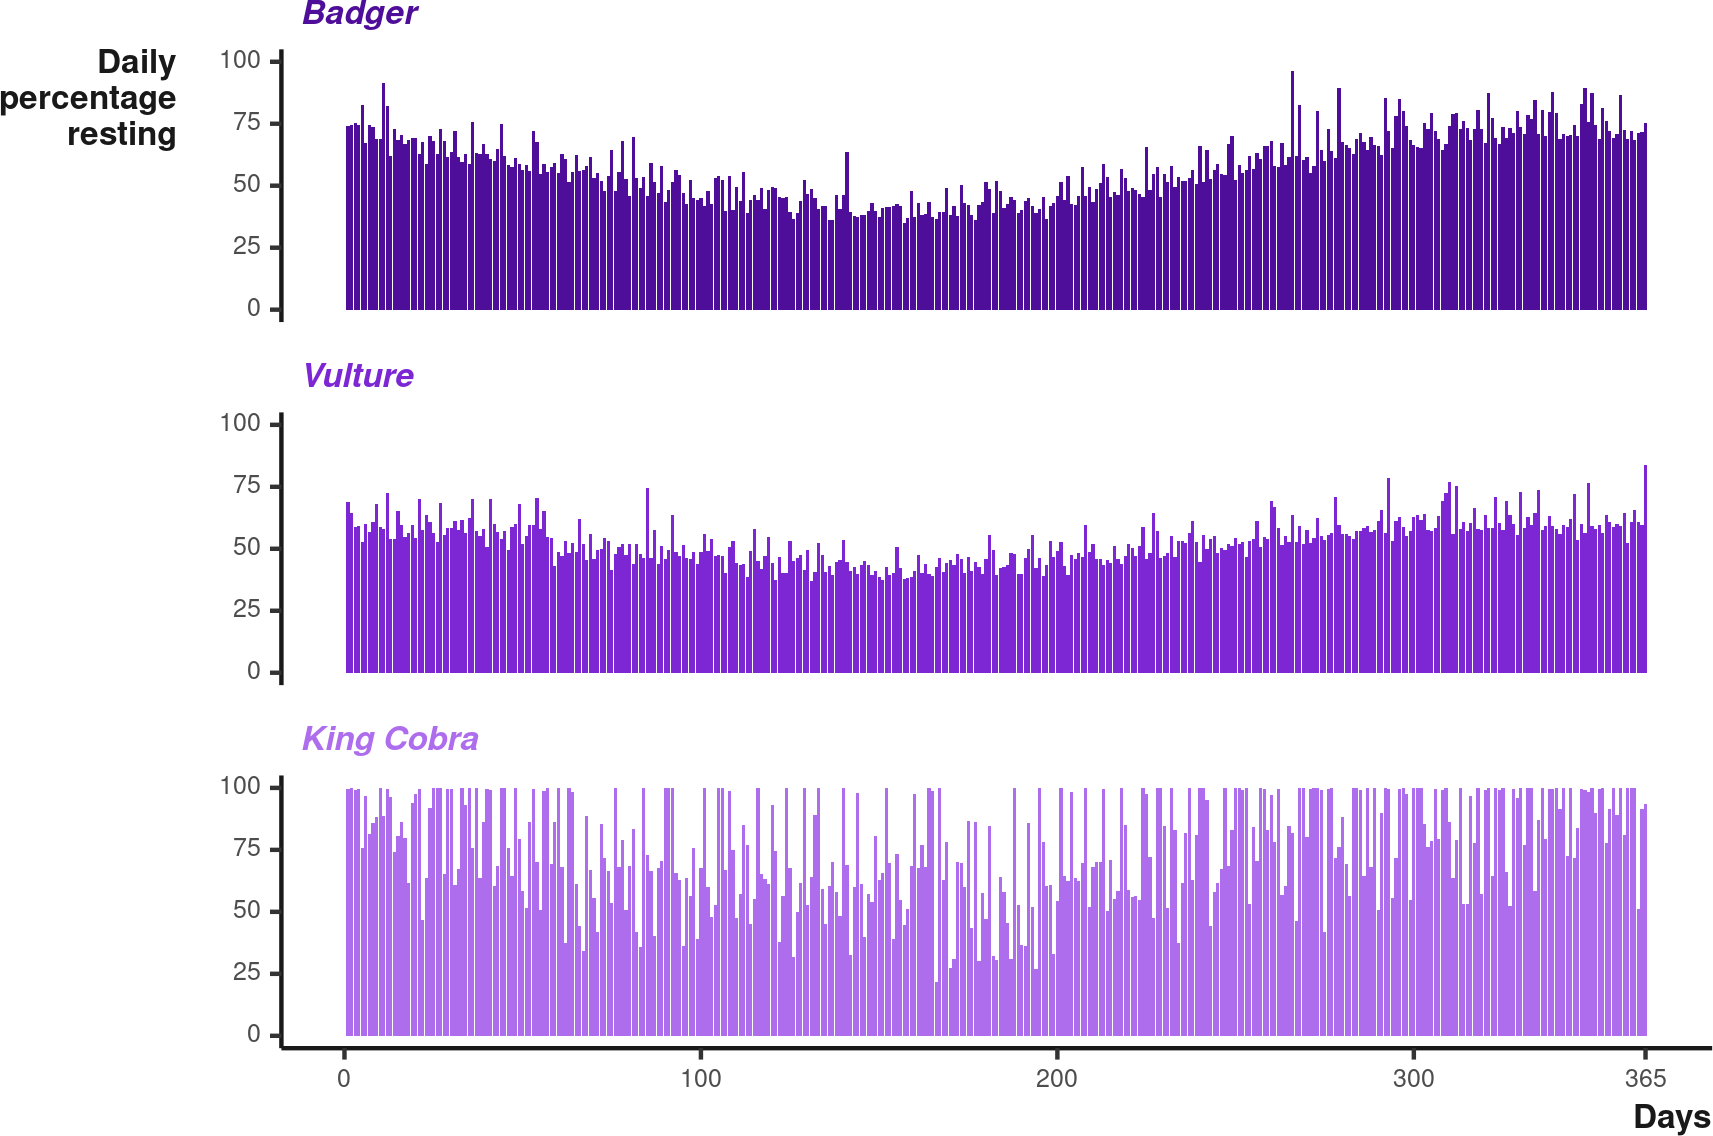
\includegraphics{Agent-based_model_walkthrough_files/figure-latex/cycleSeasonalFigure-1} 

}

\caption{The percentage of time steps spent in state 0 - resting per day, and how it varies over the entire simulated year.}\label{fig:cycleSeasonalFigure}
\end{figure}

\hypertarget{discussion}{%
\section{Discussion}\label{discussion}}

Animal movement datasets are complex and require a suite of analytical approaches to tackle satisfactorily.
Efforts to develop new, and test existing analyses would be aided by access to a range of diverse datasets.
While \emph{ideal} simulations often accompany new analysis methods --and provide superb validation for the method in question-- reaffirming the robustness and pushing those methods to new limits with a messier, more stochastic, simulation approach could greatly strength out confidence in results.
The \emph{abmAnimalMovement} package provides an independent route to test new methods that does not use an underlying mathematical movement process.

By including a range of features linked to movement and behaviour, the \emph{abmAnimalMovement} package can be implemented to investigate a suite of commonly asked of movement data --from habitat selection, to behaviour detection (for examples of common themes see \protect\hyperlink{ref-joo_recent_2022}{6}).
While some of the features can appear simplistic, there remains ample flexibility to simulate a wide range of useful scenarios.
For example, we conceptualise the three movement states as resting, exploring, and foraging.
However, only several aspects are immutable: one state exhibits site fidelity (state 0), one state is free from all attraction (state 1), and one state is driven by an underlying environmental layer (state 2).

The \emph{abmAnimalMovement} package has an advantage over data-driven simulation methods in scenarios where data is scarce, as much of the animal world is untracked (\protect\hyperlink{ref-joo_recent_2022}{6},\protect\hyperlink{ref-crane_lots_2021}{18}).
For the untracked animals we may be limited to basic information of speed, activity, and resources, or such information may even need to be inferred from ecologically similar species.
In such data starved situations, the \emph{abmAnimalMovement} package's low computational cost and minimal data requirements allows for a large number of alternative parametrisations to be explored.
Via the explorations of different parametrisations researchers can help build a picture of the study and analysis methods best suited for their questions, with the opportunity to test those analyses on synthetic simulated data.

Producing a range of simulated datasets that cover alternate scenarios may present researchers opportunities to test real data against a null model.
For example, researchers looking to investigate whether an animal was avoiding a certain landscape feature could calibrate a number of simulations covering a range of differing avoidance strengths.
The simulated results could then be compared to the real data to gauge how different the real data was from simulations exhibiting zero avoidance (i.e., a null model scenario).
This approach could compliment current analysis methods, akin to sensitivity analysis.

\hypertarget{future-directions}{%
\subsection{Future Directions}\label{future-directions}}

The \emph{abmAnimalMovement} package provides adequate functionality to simulate a range of scenarios and movements.
However, there are several aspects that will bear updating in future versions.

\begin{enumerate}
\def\labelenumi{\arabic{enumi}.}
\item
  Dynamic state 0. While state 0 and the steady state of the attraction locations is key to simulate range stability (i.e., home range), there maybe scenarios where this stability is not desired.
  For example, simulating dispersal behaviour of juvenile or sub-adult animals there may be a desire to have shelter site dynamically chosen for a time.
  Currently such behaviour could be simulated, but it would require the dispersal to occur immediately, and the dispersal destination to be predefined (i.e., the sites for state 0 attraction).
  Therefore, in the current state the package may be limited in its ability to help predict possible dispersal destination, but potentially capable of informing dispersal routes.
\item
  Autocorrelated speed. We may need to improve the autocorrelation of the animal's speed.
  Currently the speeds are non-independent based on the behavioural mode the animal is in.
  The need to implement a more aggressive movement momentum/autocorrelative structure may be felt more acutely at different time frames, and for animals with a great variation in step lengths (i.e., a larger \(\theta\) for the Gamma distribution).
  Explorations of simulated data using methods that measure autocorrelation in animal speed will reveal how much of a priority this should be.
\item
  Dynamic environment. All the environmental matrices are static, currently there is no system to update values during the simulation.
  This prevents shifts in the landscape such as seasonal variation in resources, or the development of trails.
  Currently the closest solution is to run multiple simulations where the end location of simulation\textsubscript{1} is the start location for simulation\textsubscript{2}, where simulation\textsubscript{2} is provided with a new season-appropriate resource layer.
  This solution would be inadequate for trail development, as trail development would require a system within the simulation to update previously used cells for the animal at each time step.
\end{enumerate}

\hypertarget{data-and-software-availability}{%
\section{Data and Software Availability}\label{data-and-software-availability}}

The development version of the package can be found at \href{https://github.com/BenMMarshall/abmAnimalMovement}{BenMMarshall/abmAnimalMovement}.
The stable release is available from CRAN: TBC

\hypertarget{competing-interests}{%
\section{Competing Interests}\label{competing-interests}}

No competing interests were disclosed.

\hypertarget{grant-information}{%
\section{Grant Information}\label{grant-information}}

This project was funded by the IAPETUS2 NERC DTP.

\hypertarget{acknowledgements}{%
\section{Acknowledgements}\label{acknowledgements}}

\hypertarget{author-contributions}{%
\section{Author Contributions}\label{author-contributions}}

Conceptualization: BMM;
Software: BMM;
Supervision: ABD;
Visualization: BMM;
Writing -- Original Draft: BMM;
Writing -- Review \& Editing: BMM, ABD.

\setcounter{table}{0}  \renewcommand{\thetable}{S\arabic{table}} \setcounter{figure}{0} \renewcommand{\thefigure}{S\arabic{figure}}

\hypertarget{supplementary-materials}{%
\section{Supplementary Materials}\label{supplementary-materials}}

\hypertarget{simulation-inputs}{%
\subsection{Simulation Inputs}\label{simulation-inputs}}

\hypertarget{palette}{%
\subsubsection{Palette}\label{palette}}

\begin{figure}

{\centering 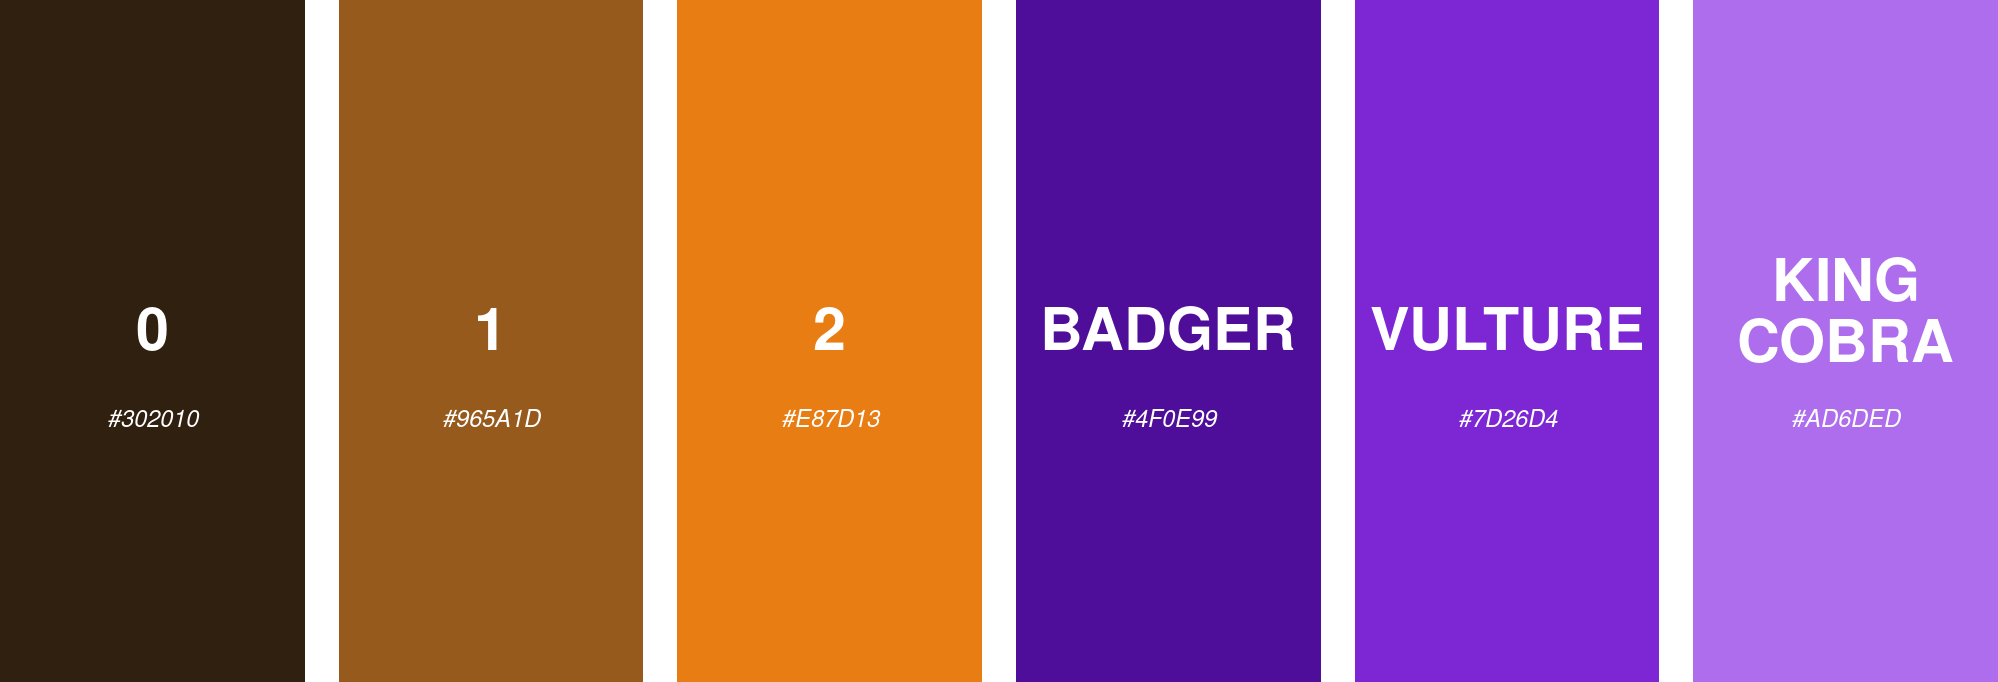
\includegraphics{Agent-based_model_walkthrough_files/figure-latex/palettePreview-1} 

}

\caption{Universal colour key for behavioural states 0 - resting, 1 - foraging, 2 - exploring; and example species. Name assigned to the colour in bold, and the hex code in italics below.}\label{fig:palettePreview}
\end{figure}

\hypertarget{vulture-inputs}{%
\subsubsection{Vulture Inputs}\label{vulture-inputs}}

Values input to generate more vulture-like movement patterns.

\begin{Shaded}
\begin{Highlighting}[]
\NormalTok{VULTURE\_shelterLocs }\OtherTok{\textless{}{-}} \FunctionTok{data.frame}\NormalTok{(}
  \StringTok{"x"} \OtherTok{=} \FunctionTok{c}\NormalTok{(}\DecValTok{1024}\NormalTok{, }\DecValTok{1005}\NormalTok{, }\DecValTok{1115}\NormalTok{),}
  \StringTok{"y"} \OtherTok{=} \FunctionTok{c}\NormalTok{(}\DecValTok{1193}\NormalTok{, }\DecValTok{1070}\NormalTok{, }\DecValTok{882}\NormalTok{))}

\NormalTok{VULTURE\_shelterSize }\OtherTok{\textless{}{-}} \DecValTok{5}


\NormalTok{VULTURE\_k\_step }\OtherTok{\textless{}{-}} \FunctionTok{c}\NormalTok{(}\DecValTok{2}\NormalTok{, }\FloatTok{2.2}\SpecialCharTok{*}\DecValTok{60}\NormalTok{, }\FloatTok{1.5}\SpecialCharTok{*}\DecValTok{60}\NormalTok{)}
\NormalTok{VULTURE\_s\_step }\OtherTok{\textless{}{-}} \FunctionTok{c}\NormalTok{(}\DecValTok{40}\NormalTok{, }\FloatTok{1.2}\NormalTok{, }\DecValTok{1}\NormalTok{)}
\NormalTok{VULTURE\_mu\_angle }\OtherTok{\textless{}{-}} \FunctionTok{c}\NormalTok{(}\DecValTok{0}\NormalTok{, }\DecValTok{0}\NormalTok{, }\DecValTok{0}\NormalTok{)}
\NormalTok{VULTURE\_k\_angle }\OtherTok{\textless{}{-}} \FunctionTok{c}\NormalTok{(}\FloatTok{0.6}\NormalTok{, }\FloatTok{0.99}\NormalTok{, }\FloatTok{0.6}\NormalTok{)}

\NormalTok{VULTURE\_destinationRange }\OtherTok{\textless{}{-}} \FunctionTok{c}\NormalTok{(}\DecValTok{50}\NormalTok{, }\DecValTok{120}\NormalTok{)}
\NormalTok{VULTURE\_destinationDirection }\OtherTok{\textless{}{-}} \FunctionTok{c}\NormalTok{(}\DecValTok{0}\NormalTok{, }\FloatTok{0.01}\NormalTok{)}
\NormalTok{VULTURE\_destinationTransformation }\OtherTok{\textless{}{-}} \DecValTok{2}
\NormalTok{VULTURE\_destinationModifier }\OtherTok{\textless{}{-}} \DecValTok{2}

\NormalTok{VULTURE\_rescale }\OtherTok{\textless{}{-}} \DecValTok{20}


\NormalTok{VULTURE\_rest\_Cycle }\OtherTok{\textless{}{-}} \FunctionTok{c}\NormalTok{(}\FloatTok{0.42}\NormalTok{, }\FloatTok{0.1}\NormalTok{, }\DecValTok{24}\NormalTok{, }\DecValTok{24}\NormalTok{)}

\DocumentationTok{\#\# multiple cycle additions}
\NormalTok{c0 }\OtherTok{\textless{}{-}} \FunctionTok{c}\NormalTok{(}\FloatTok{0.12}\NormalTok{, }\SpecialCharTok{{-}}\FloatTok{0.05}\NormalTok{, }\DecValTok{24}\SpecialCharTok{*}\NormalTok{ (}\DecValTok{365}\SpecialCharTok{/}\DecValTok{2}\NormalTok{), }\DecValTok{24}\SpecialCharTok{*} \DecValTok{365}\NormalTok{) }\CommentTok{\# seasonal}

\NormalTok{VULTURE\_additional\_Cycles }\OtherTok{\textless{}{-}} \FunctionTok{rbind}\NormalTok{(c0)}

\NormalTok{VULTURE\_behaveMatrix }\OtherTok{\textless{}{-}}\NormalTok{ Default\_behaveMatrix}
\NormalTok{VULTURE\_behaveMatrix[}\DecValTok{2}\NormalTok{,}\DecValTok{2}\NormalTok{] }\OtherTok{\textless{}{-}} \FloatTok{0.990}
\NormalTok{VULTURE\_behaveMatrix[}\DecValTok{2}\NormalTok{,}\DecValTok{3}\NormalTok{] }\OtherTok{\textless{}{-}} \FloatTok{0.01}
\NormalTok{VULTURE\_behaveMatrix[}\DecValTok{3}\NormalTok{,}\DecValTok{2}\NormalTok{] }\OtherTok{\textless{}{-}} \FloatTok{0.05}
\NormalTok{VULTURE\_behaveMatrix[}\DecValTok{1}\NormalTok{,}\DecValTok{1}\NormalTok{] }\OtherTok{\textless{}{-}} \FloatTok{0.85}
\NormalTok{VULTURE\_behaveMatrix[}\DecValTok{1}\NormalTok{,}\DecValTok{2}\NormalTok{] }\OtherTok{\textless{}{-}} \FloatTok{0.01}


\NormalTok{VULTURE\_movementMatrix }\OtherTok{\textless{}{-}}\NormalTok{ landscapeLayersList}\SpecialCharTok{$}\NormalTok{movement}
\NormalTok{VULTURE\_movementMatrix[] }\OtherTok{\textless{}{-}} \DecValTok{1}


\NormalTok{VULTURE\_forageMatrix }\OtherTok{\textless{}{-}}\NormalTok{ landscapeLayersList}\SpecialCharTok{$}\NormalTok{forage}
\NormalTok{VULTURE\_forageMatrix[}\DecValTok{1}\SpecialCharTok{:}\DecValTok{950}\NormalTok{,}\DecValTok{1}\SpecialCharTok{:}\DecValTok{2000}\NormalTok{] }\OtherTok{\textless{}{-}}\NormalTok{ VULTURE\_forageMatrix[}\DecValTok{1}\SpecialCharTok{:}\DecValTok{950}\NormalTok{,}\DecValTok{1}\SpecialCharTok{:}\DecValTok{2000}\NormalTok{] }\SpecialCharTok{{-}} \FloatTok{0.6}
\NormalTok{VULTURE\_forageMatrix[VULTURE\_forageMatrix[] }\SpecialCharTok{\textless{}} \DecValTok{0}\NormalTok{] }\OtherTok{\textless{}{-}} \DecValTok{0}
\end{Highlighting}
\end{Shaded}

\begin{figure}

{\centering 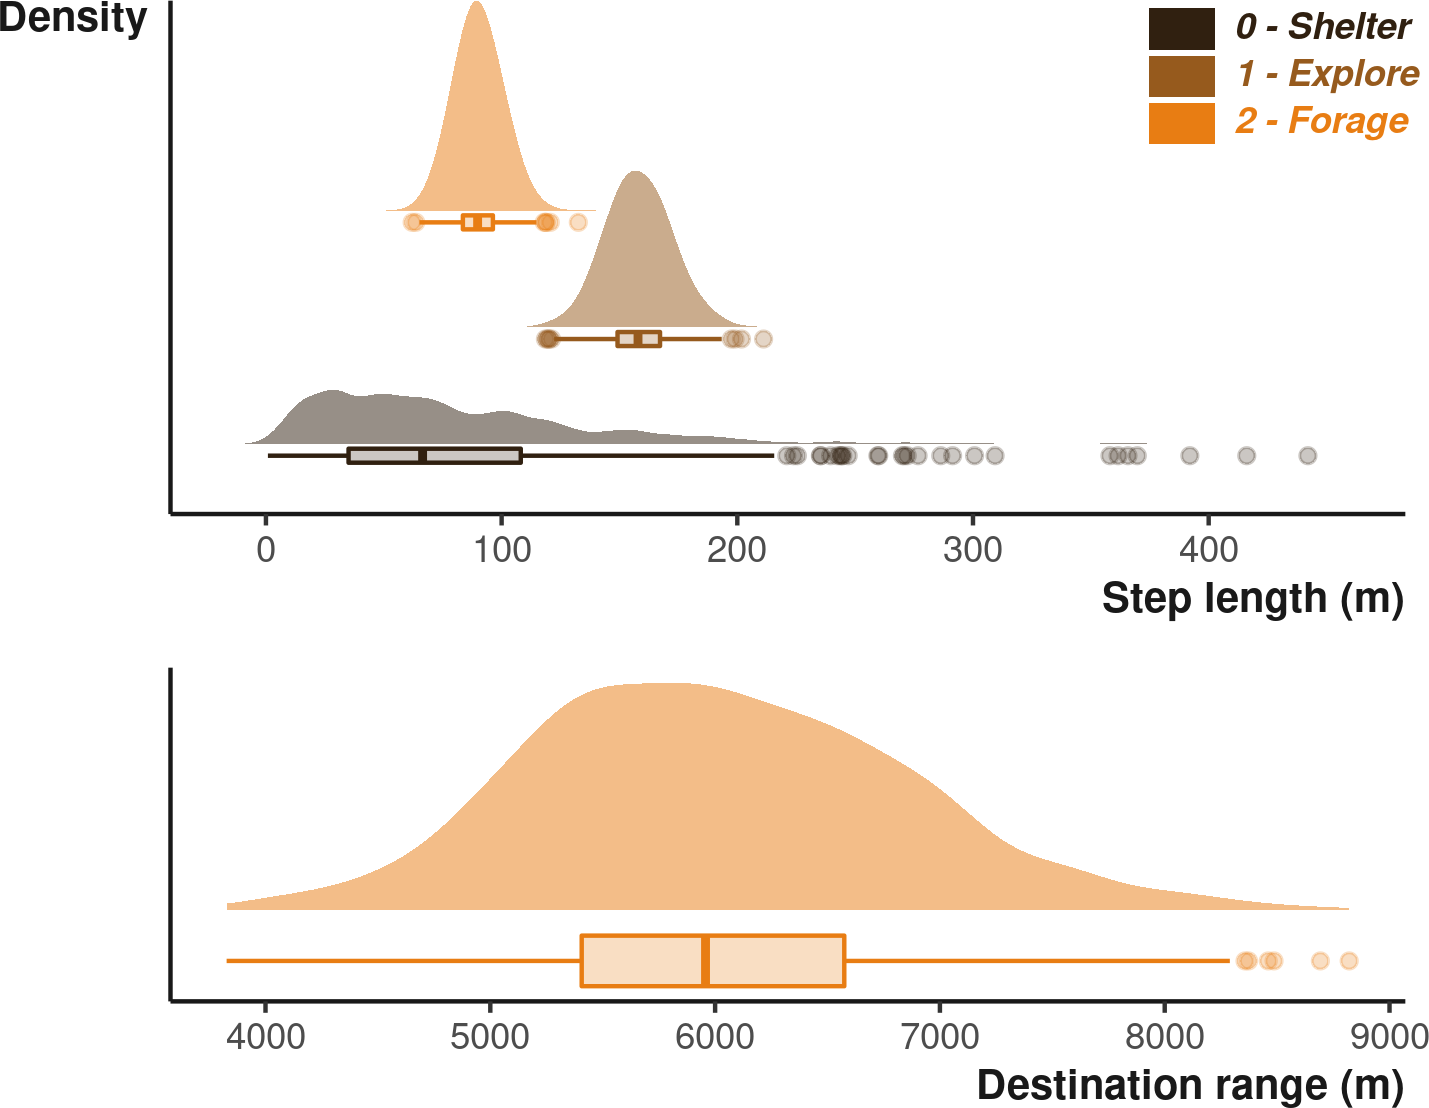
\includegraphics{Agent-based_model_walkthrough_files/figure-latex/VULTUREsettingMoveDesPlot-1} 

}

\caption{The distribution of step lengths, and corresponding box plot for the vulture example. The lower plot shows the distribution used to generate potential foraging desintations.}\label{fig:VULTUREsettingMoveDesPlot}
\end{figure}

\begin{figure}

{\centering 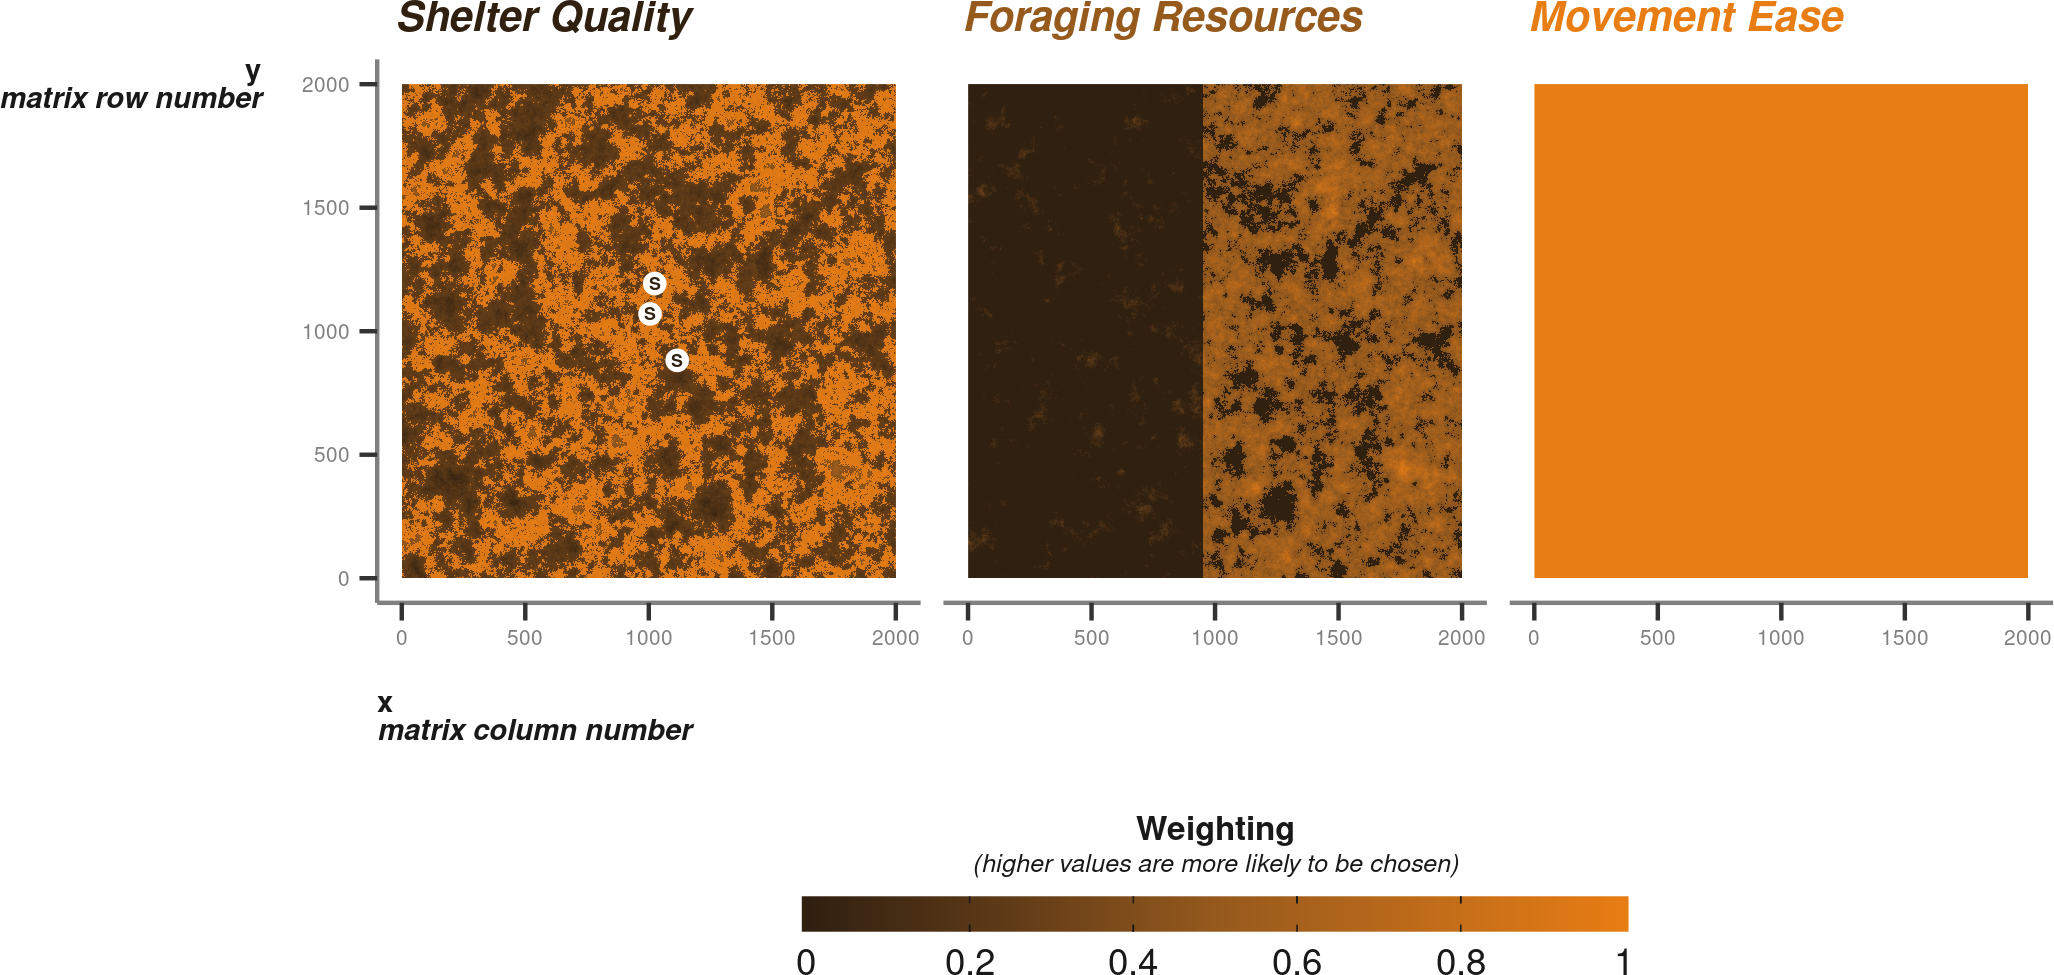
\includegraphics{Agent-based_model_walkthrough_files/figure-latex/VULTURElayersFigure-1} 

}

\caption{The three resulting landscape layers to be fed into the simulation for the vulture example: shelter quality, foraging resources, movement ease.}\label{fig:VULTURElayersFigure}
\end{figure}

\hypertarget{king-cobra-inputs}{%
\subsubsection{King Cobra Inputs}\label{king-cobra-inputs}}

Values input to generate more king cobra-like movement patterns.

\begin{Shaded}
\begin{Highlighting}[]
\NormalTok{sampledShelters }\OtherTok{\textless{}{-}} \FunctionTok{sampleRandom}\NormalTok{(}\FunctionTok{raster}\NormalTok{(landscapeLayersList}\SpecialCharTok{$}\NormalTok{shelter), }\DecValTok{12}\NormalTok{,}
                                \AttributeTok{ext =} \FunctionTok{extent}\NormalTok{(}\FloatTok{0.35}\NormalTok{, }\FloatTok{0.65}\NormalTok{, }\FloatTok{0.35}\NormalTok{, }\FloatTok{0.65}\NormalTok{), }
                                \AttributeTok{rowcol =} \ConstantTok{TRUE}\NormalTok{)}

\NormalTok{KINGCOBRA\_shelterLocs }\OtherTok{\textless{}{-}} \FunctionTok{data.frame}\NormalTok{(}
  \StringTok{"x"} \OtherTok{=}\NormalTok{ sampledShelters[,}\DecValTok{2}\NormalTok{],}
  \StringTok{"y"} \OtherTok{=}\NormalTok{ sampledShelters[,}\DecValTok{1}\NormalTok{])}

\NormalTok{KINGCOBRA\_shelterSize }\OtherTok{\textless{}{-}} \DecValTok{10}


\NormalTok{KINGCOBRA\_k\_step }\OtherTok{\textless{}{-}} \FunctionTok{c}\NormalTok{(}\DecValTok{30}\NormalTok{, }\DecValTok{40}\NormalTok{, }\DecValTok{20}\NormalTok{)}
\NormalTok{KINGCOBRA\_s\_step }\OtherTok{\textless{}{-}} \FunctionTok{c}\NormalTok{(}\FloatTok{0.75}\NormalTok{, }\FloatTok{1.2}\NormalTok{, }\FloatTok{1.75}\NormalTok{)}
\NormalTok{KINGCOBRA\_mu\_angle }\OtherTok{\textless{}{-}} \FunctionTok{c}\NormalTok{(}\DecValTok{0}\NormalTok{, }\DecValTok{0}\NormalTok{, }\DecValTok{0}\NormalTok{)}
\NormalTok{KINGCOBRA\_k\_angle }\OtherTok{\textless{}{-}} \FunctionTok{c}\NormalTok{(}\FloatTok{0.6}\NormalTok{, }\FloatTok{0.99}\NormalTok{, }\FloatTok{0.6}\NormalTok{)}

\NormalTok{KINGCOBRA\_destinationRange }\OtherTok{\textless{}{-}} \FunctionTok{c}\NormalTok{(}\DecValTok{50}\NormalTok{, }\DecValTok{10}\NormalTok{)}
\NormalTok{KINGCOBRA\_destinationDirection }\OtherTok{\textless{}{-}} \FunctionTok{c}\NormalTok{(}\DecValTok{0}\NormalTok{, }\FloatTok{0.01}\NormalTok{)}
\NormalTok{KINGCOBRA\_destinationTransformation }\OtherTok{\textless{}{-}} \DecValTok{2}
\NormalTok{KINGCOBRA\_destinationModifier }\OtherTok{\textless{}{-}} \FloatTok{1.5}

\NormalTok{KINGCOBRA\_rescale }\OtherTok{\textless{}{-}} \DecValTok{4}


\NormalTok{KINGCOBRA\_rest\_Cycle }\OtherTok{\textless{}{-}} \FunctionTok{c}\NormalTok{(}\FloatTok{0.25}\NormalTok{, }\DecValTok{0}\NormalTok{, }\DecValTok{24}\NormalTok{, }\DecValTok{24}\NormalTok{)}

\DocumentationTok{\#\# multiple cycle additions}
\NormalTok{c0 }\OtherTok{\textless{}{-}} \FunctionTok{c}\NormalTok{(}\FloatTok{0.2}\NormalTok{, }\DecValTok{0}\NormalTok{, }\DecValTok{24}\NormalTok{, }\DecValTok{24}\SpecialCharTok{*}\DecValTok{4}\NormalTok{) }\CommentTok{\# digest}
\NormalTok{c1 }\OtherTok{\textless{}{-}} \FunctionTok{c}\NormalTok{(}\FloatTok{0.1}\NormalTok{, }\DecValTok{0}\NormalTok{, }\DecValTok{24} \SpecialCharTok{*}\NormalTok{ (}\DecValTok{365}\SpecialCharTok{/}\DecValTok{2}\NormalTok{), }\DecValTok{24}\SpecialCharTok{*} \DecValTok{365}\NormalTok{ ) }\CommentTok{\# seasonal}

\NormalTok{KINGCOBRA\_additional\_Cycles }\OtherTok{\textless{}{-}} \FunctionTok{rbind}\NormalTok{(c0, c1)}


\NormalTok{KINGCOBRA\_movementMatrix }\OtherTok{\textless{}{-}}\NormalTok{ landscapeLayersList}\SpecialCharTok{$}\NormalTok{movement}

\CommentTok{\# two strong intersections hampering movement}
\NormalTok{KINGCOBRA\_movementMatrix[}\DecValTok{1200}\SpecialCharTok{:}\DecValTok{1240}\NormalTok{,}\DecValTok{1}\SpecialCharTok{:}\DecValTok{2000}\NormalTok{] }\OtherTok{\textless{}{-}}\NormalTok{ KINGCOBRA\_movementMatrix[}\DecValTok{1200}\SpecialCharTok{:}\DecValTok{1240}\NormalTok{,}\DecValTok{1}\SpecialCharTok{:}\DecValTok{2000}\NormalTok{] }\SpecialCharTok{{-}} \FloatTok{0.95}
\NormalTok{KINGCOBRA\_movementMatrix[}\DecValTok{1}\SpecialCharTok{:}\DecValTok{2000}\NormalTok{,}\DecValTok{850}\SpecialCharTok{:}\DecValTok{890}\NormalTok{] }\OtherTok{\textless{}{-}}\NormalTok{ KINGCOBRA\_movementMatrix[}\DecValTok{1}\SpecialCharTok{:}\DecValTok{2000}\NormalTok{,}\DecValTok{850}\SpecialCharTok{:}\DecValTok{890}\NormalTok{] }\SpecialCharTok{{-}} \FloatTok{0.95}
\NormalTok{KINGCOBRA\_movementMatrix[KINGCOBRA\_movementMatrix[] }\SpecialCharTok{\textless{}} \DecValTok{0}\NormalTok{] }\OtherTok{\textless{}{-}} \DecValTok{0}

\NormalTok{KINGCOBRA\_avoidLocs }\OtherTok{\textless{}{-}} \FunctionTok{data.frame}\NormalTok{(}
  \StringTok{"x"} \OtherTok{=} \FunctionTok{c}\NormalTok{(}\DecValTok{552}\NormalTok{, }\DecValTok{1232}\NormalTok{, }\DecValTok{1587}\NormalTok{),}
  \StringTok{"y"} \OtherTok{=} \FunctionTok{c}\NormalTok{(}\DecValTok{789}\NormalTok{, }\DecValTok{975}\NormalTok{, }\DecValTok{1356}\NormalTok{))}

\NormalTok{KINGCOBRA\_avoidTransformation }\OtherTok{\textless{}{-}} \DecValTok{2}
\NormalTok{KINGCOBRA\_avoidModifier }\OtherTok{\textless{}{-}} \DecValTok{1}
\end{Highlighting}
\end{Shaded}

\begin{figure}

{\centering 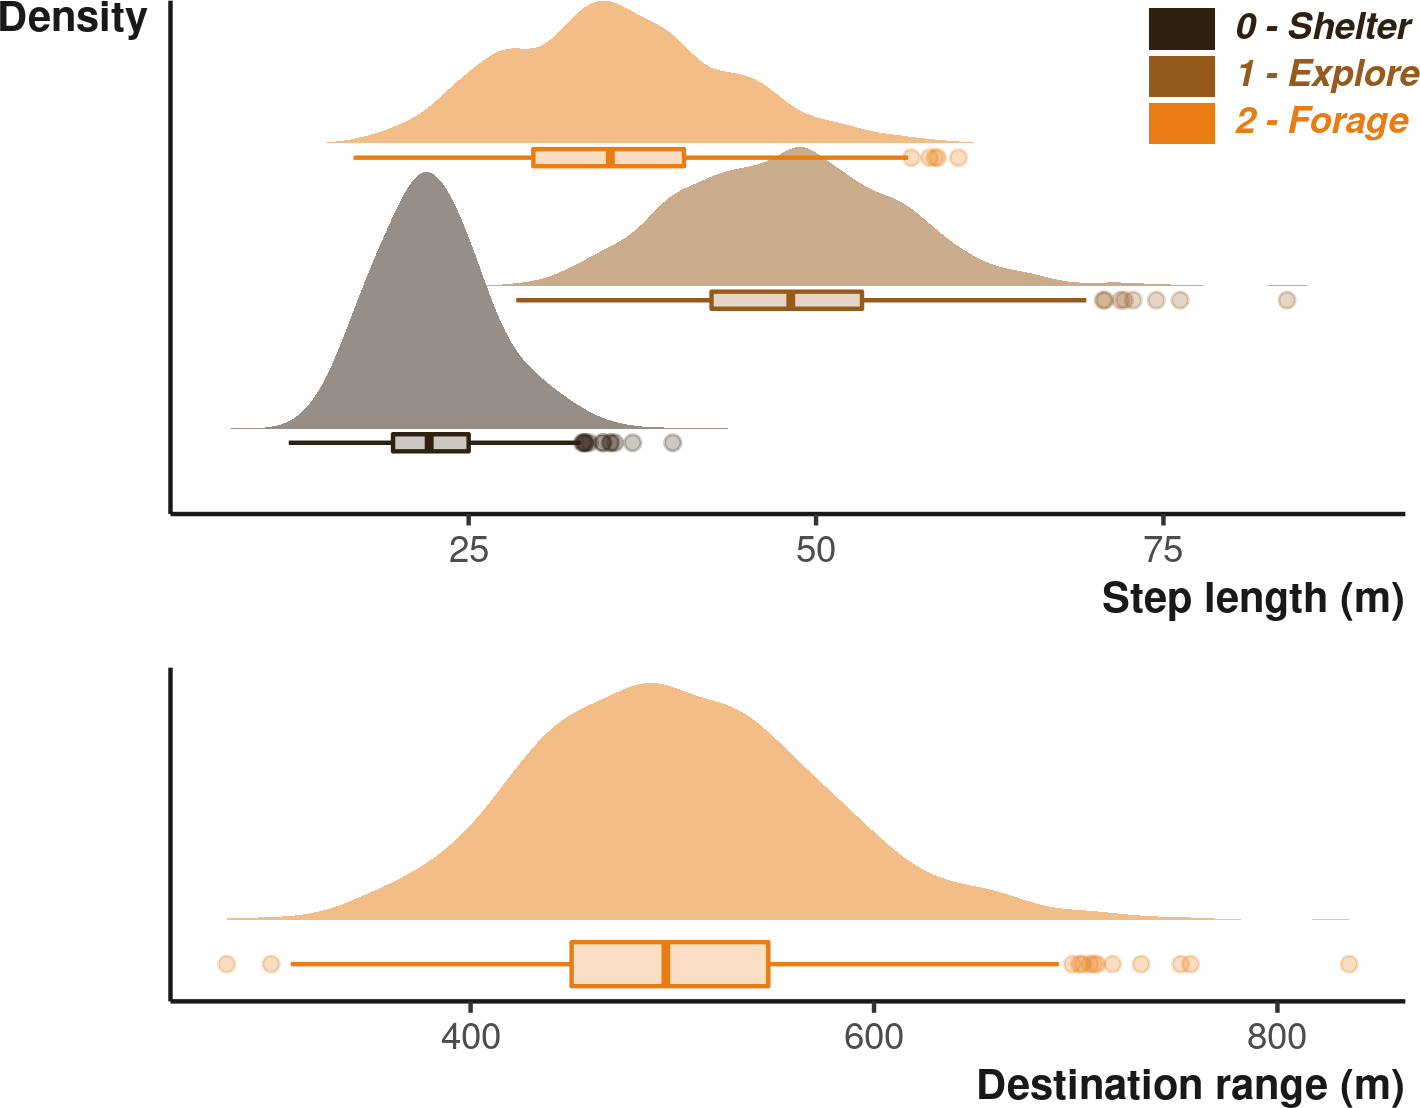
\includegraphics{Agent-based_model_walkthrough_files/figure-latex/KINGCOBRAsettingMoveDesPlot-1} 

}

\caption{The distribution of step lengths, and corresponding box plot for the king cobra example. The lower plot shows the distribution used to generate potential foraging desintations.}\label{fig:KINGCOBRAsettingMoveDesPlot}
\end{figure}

\begin{figure}

{\centering 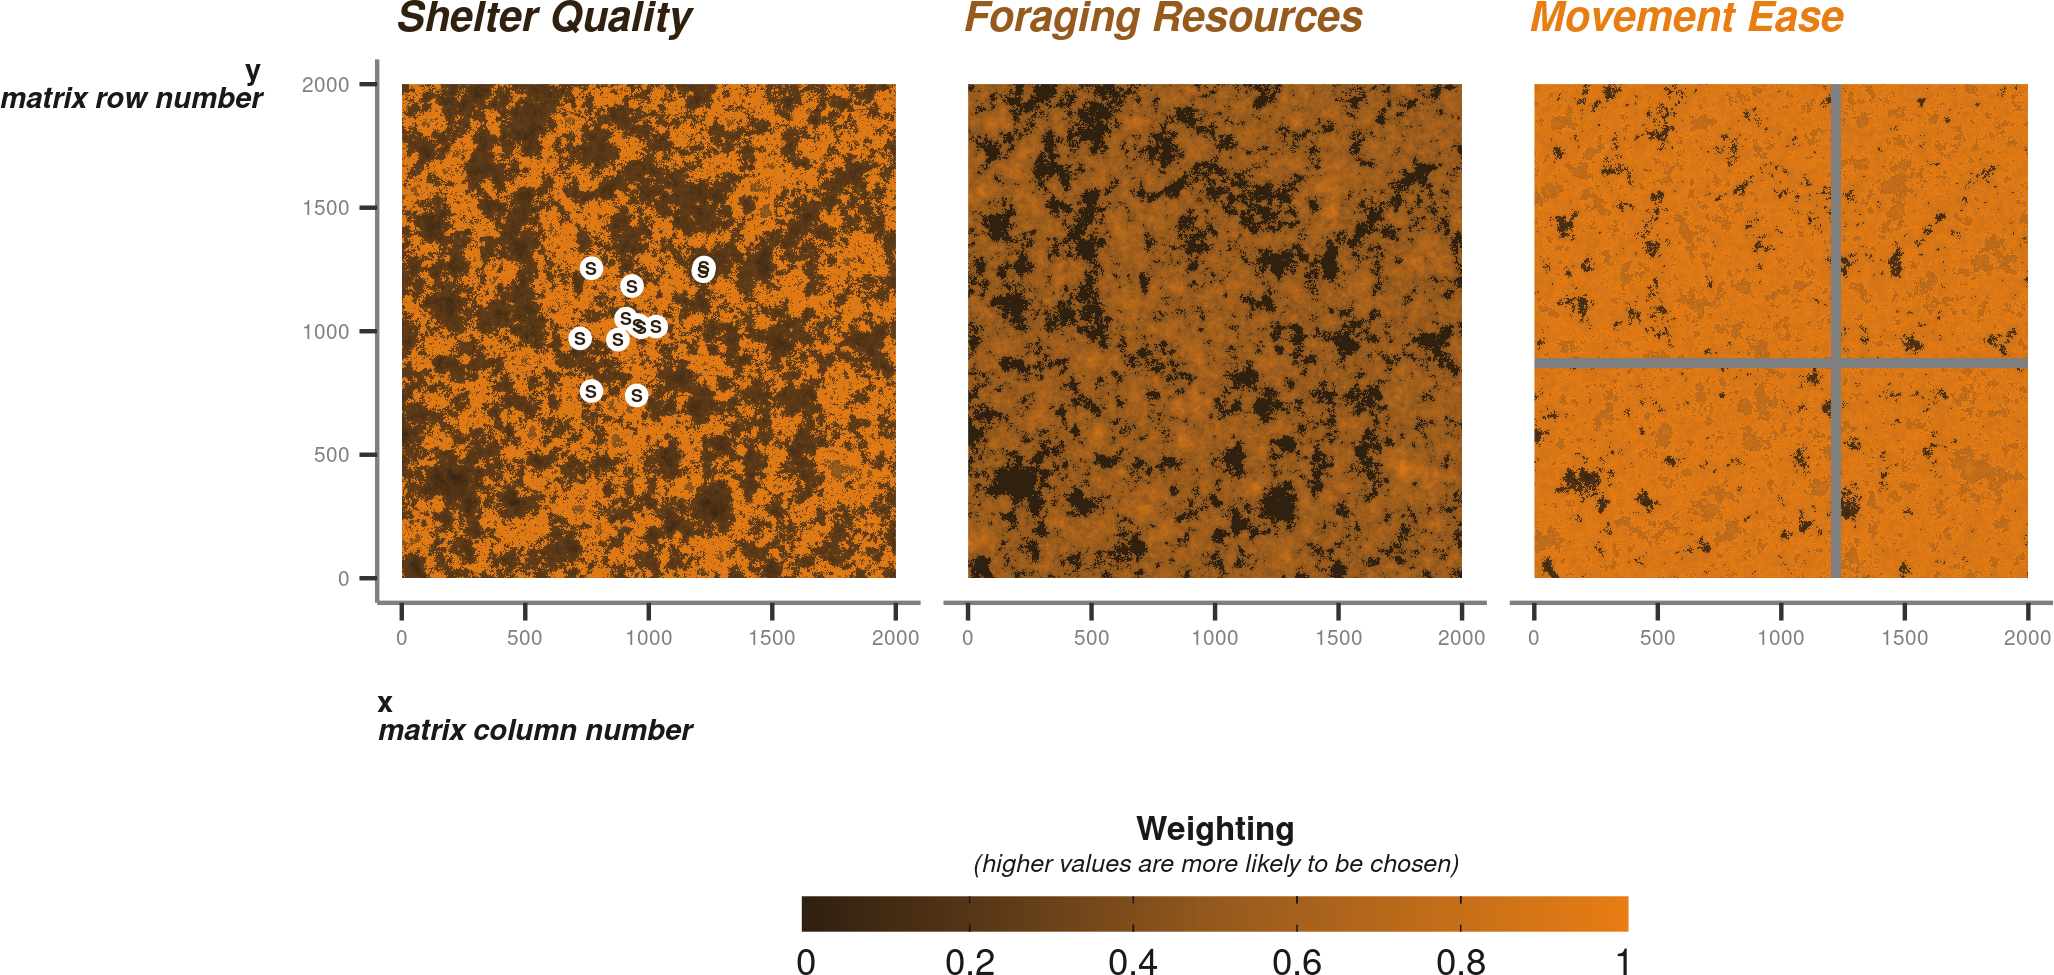
\includegraphics{Agent-based_model_walkthrough_files/figure-latex/KINGCOBRAlayersFigure-1} 

}

\caption{The three resulting landscape layers to be fed into the simulation for the king cobra example: shelter quality, foraging resources, movement ease.}\label{fig:KINGCOBRAlayersFigure}
\end{figure}

\clearpage

\hypertarget{simulation-outputs}{%
\subsection{Simulation Outputs}\label{simulation-outputs}}

Figures \ref{fig:VULTUREsettingMoveDesPlot} and \ref{fig:KINGCOBRAsettingMoveDesPlot} describe the inputs for the vulture and king cobra example respectively, and are comparable to figures \ref{fig:VULTUREmoveCharFigure} and \ref{fig:KINGCOBRAmoveCharFigure}.
Figures \ref{fig:BADGERmoveCharFigure}, \ref{fig:VULTUREmoveCharFigure}, and \ref{fig:KINGCOBRAmoveCharFigure} also provide information on the rates of stationary behaviour, defined in the plot as step lengths less than the shelter site size.
The King Cobra example in particular highlights the prolonged near weekly resting periods.

\begin{figure}

{\centering 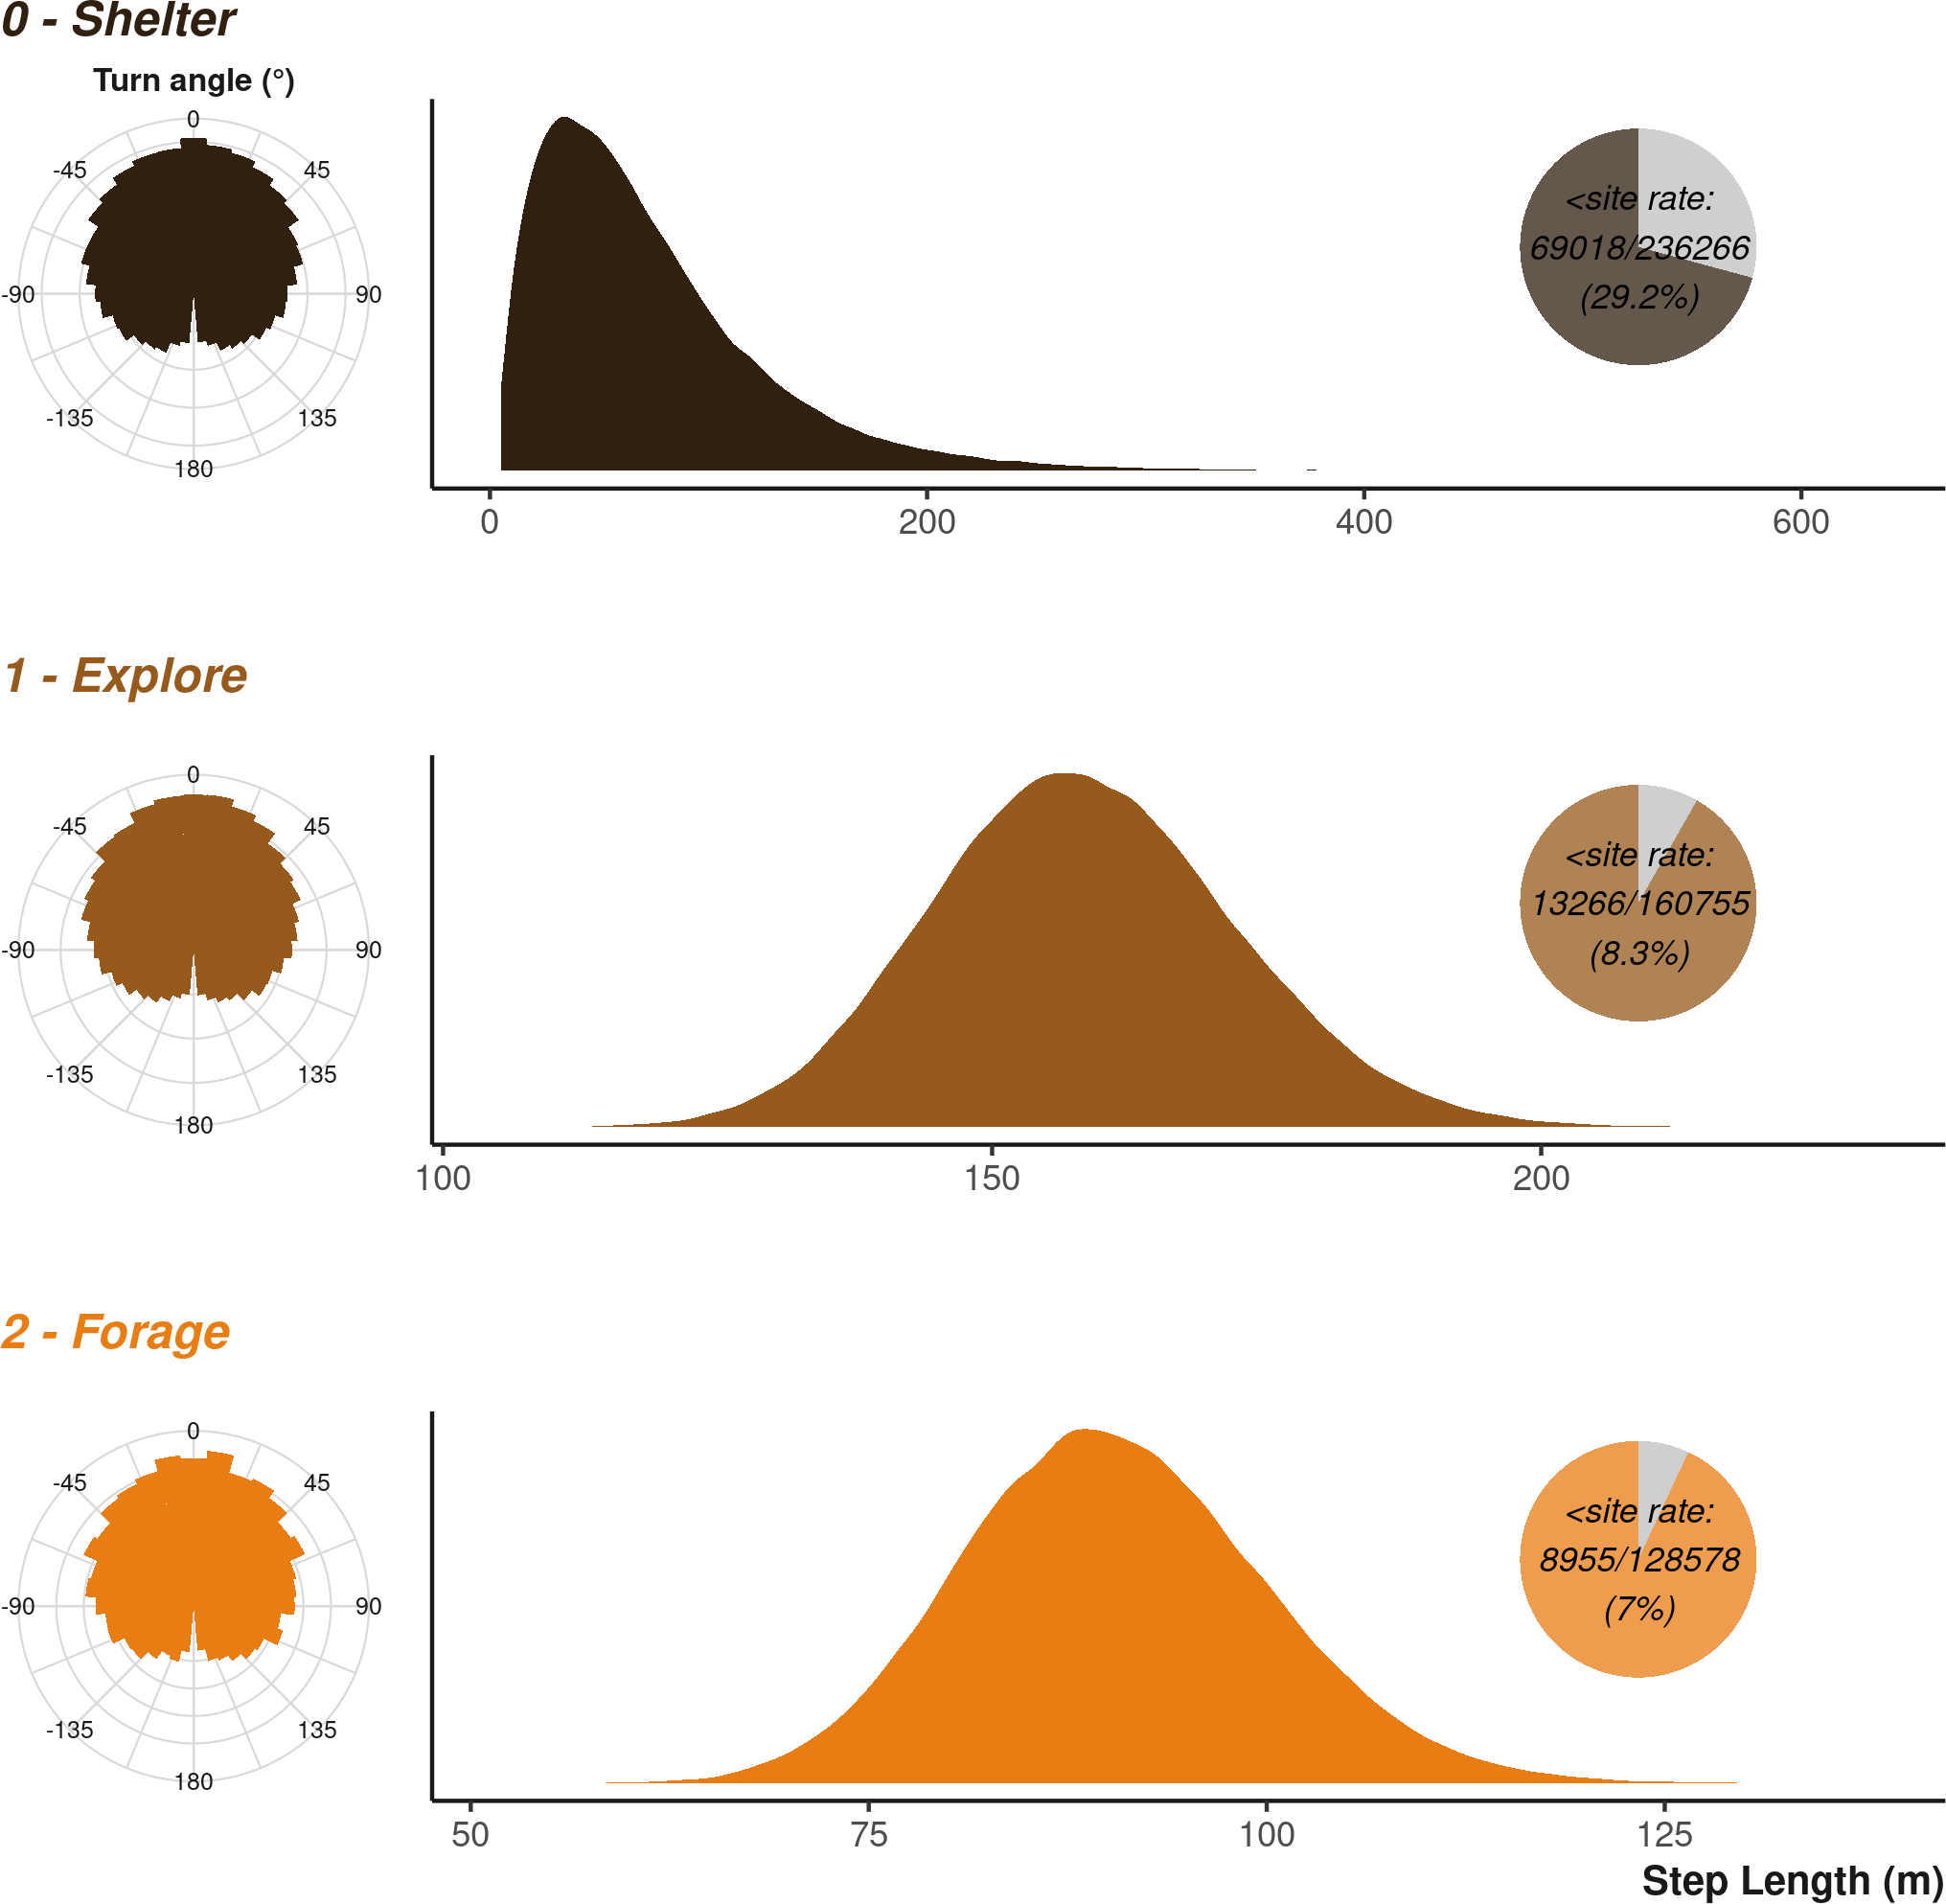
\includegraphics{Agent-based_model_walkthrough_files/figure-latex/VULTUREmoveCharFigure-1} 

}

\caption{The vulture example's observed turn angles and step lengths resulting from the simulation. Step lengths are scaled back to the input units. Inset pie chart show the number of step lengths that were below the shelter site size; the sub-shelter site step lengths are excluded from the density plot. Note that x axis is not consistent between the three plots.}\label{fig:VULTUREmoveCharFigure}
\end{figure}

\begin{figure}

{\centering 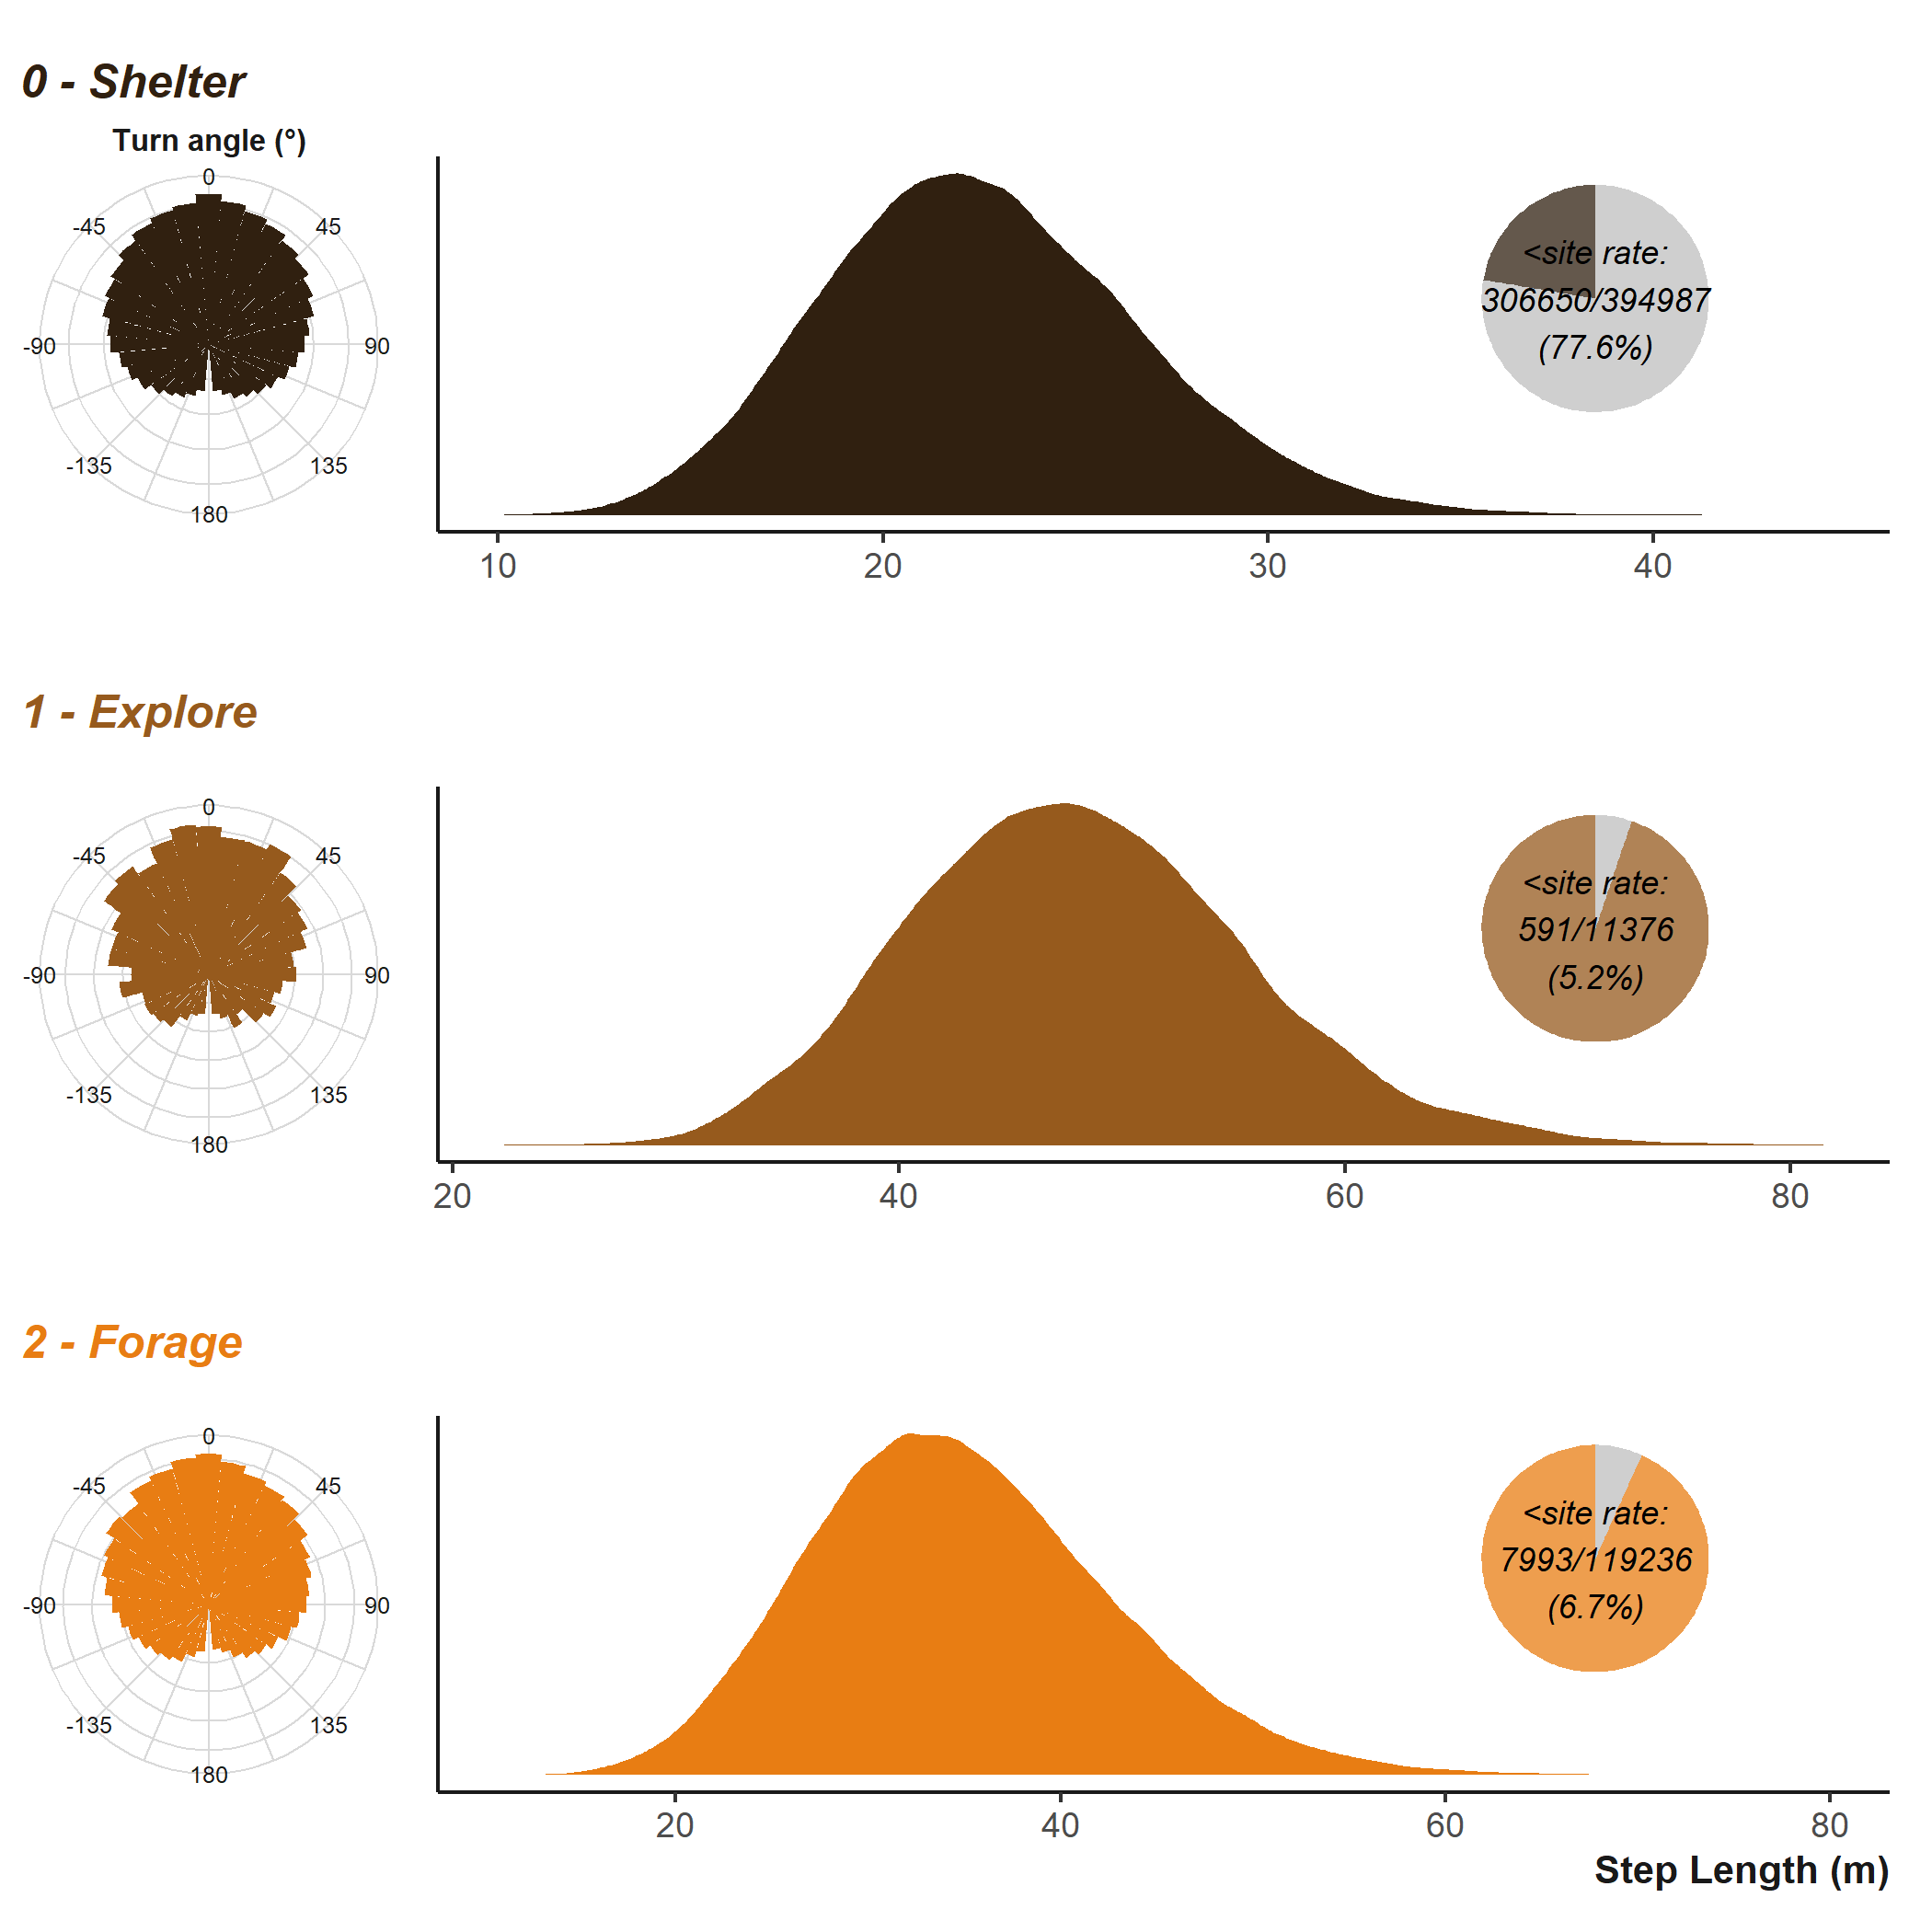
\includegraphics{Agent-based_model_walkthrough_files/figure-latex/KINGCOBRAmoveCharFigure-1} 

}

\caption{The king cobra example's observed turn angles and step lengths resulting from the simulation. Step lengths are scaled back to the input units. Inset pie chart show the number of step lengths that were below the shelter site size; the sub-shelter site step lengths are excluded from the density plot. Note that x axis is not consistent between the three plots.}\label{fig:KINGCOBRAmoveCharFigure}
\end{figure}

\clearpage

\hypertarget{references}{%
\section*{References}\label{references}}
\addcontentsline{toc}{section}{References}

\hypertarget{refs}{}
\begin{CSLReferences}{0}{0}
\leavevmode\vadjust pre{\hypertarget{ref-Bastille-Rousseau2017}{}}%
\CSLLeftMargin{1. }
\CSLRightInline{Bastille-Rousseau G, Murray DL, Schaefer JA, Lewis MA, Mahoney SP, Potts JR. \href{https://doi.org/10.1111/ecog.02655}{Spatial scales of habitat selection decisions: {Implications} for telemetry-based movement modelling}. Ecography. 2017;40:1--7. }

\leavevmode\vadjust pre{\hypertarget{ref-sridhar_geometry_2021}{}}%
\CSLLeftMargin{2. }
\CSLRightInline{Sridhar VH, Li L, Gorbonos D, Nagy M, Schell BR, Sorochkin T, et al. The geometry of decision-making in individuals and collectives. Proceedings of the National Academy of Sciences {[}Internet{]}. 2021 Dec {[}cited 2022 May 3{]};118(50):e2102157118. Available from: \url{https://pnas.org/doi/full/10.1073/pnas.2102157118}}

\leavevmode\vadjust pre{\hypertarget{ref-Fraser2018}{}}%
\CSLLeftMargin{3. }
\CSLRightInline{Fraser KC, Davies KT, Davy CM, Ford AT, Flockhart DTT, Martins EG. Tracking the conservation promise of movement ecology. Frontiers in Ecology and Evolution {[}Internet{]}. 2018;6(October):150. Available from: \url{https://www.frontiersin.org/articles/10.3389/fevo.2018.00150/full?utm_source=F-NTF\&utm_medium=EMLX\&utm_campaign=PRD_FEOPS_20170000_ARTICLE}}

\leavevmode\vadjust pre{\hypertarget{ref-noonan_effects_2020}{}}%
\CSLLeftMargin{4. }
\CSLRightInline{Noonan MJ, Fleming CH, Tucker MA, Kays R, Harrison A, Crofoot MC, et al. Effects of body size on estimation of mammalian area requirements. Conservation Biology {[}Internet{]}. 2020 Jun {[}cited 2020 Jun 23{]};cobi.13495. Available from: \url{https://onlinelibrary.wiley.com/doi/abs/10.1111/cobi.13495}}

\leavevmode\vadjust pre{\hypertarget{ref-studd_purrfect_2021}{}}%
\CSLLeftMargin{5. }
\CSLRightInline{Studd EK, Derbyshire RE, Menzies AK, Simms JF, Humphries MM, Murray DL, et al. The {Purr}‐fect {Catch}: {Using} accelerometers and audio recorders to document kill rates and hunting behaviour of a small prey specialist. Methods in Ecology and Evolution {[}Internet{]}. 2021 Jul {[}cited 2022 May 25{]};12(7):1277--87. Available from: \url{https://onlinelibrary.wiley.com/doi/10.1111/2041-210X.13605}}

\leavevmode\vadjust pre{\hypertarget{ref-joo_recent_2022}{}}%
\CSLLeftMargin{6. }
\CSLRightInline{Joo R, Picardi S, Boone ME, Clay TA, Patrick SC, Romero-Romero VS, et al. Recent trends in movement ecology of animals and human mobility. Movement Ecology {[}Internet{]}. 2022 May {[}cited 2022 Jun 3{]};10(1):26. Available from: \url{https://doi.org/10.1186/s40462-022-00322-9}}

\leavevmode\vadjust pre{\hypertarget{ref-wild_internet_2022}{}}%
\CSLLeftMargin{7. }
\CSLRightInline{Wild TA, Wikelski M, Tyndel S, Alarcón‐Nieto G, Klump BC, Aplin LM, et al. Internet on animals: {Wi}‐{Fi}‐enabled devices provide a solution for big data transmission in biologging. Methods in Ecology and Evolution {[}Internet{]}. 2022 Jan {[}cited 2022 May 25{]};2041--210X.13798. Available from: \url{https://onlinelibrary.wiley.com/doi/10.1111/2041-210X.13798}}

\leavevmode\vadjust pre{\hypertarget{ref-kays_movebank_2022}{}}%
\CSLLeftMargin{8. }
\CSLRightInline{Kays R, Davidson SC, Berger M, Bohrer G, Fiedler W, Flack A, et al. The {Movebank} system for studying global animal movement and demography. Methods in Ecology and Evolution {[}Internet{]}. 2022 Feb {[}cited 2022 May 25{]};13(2):419--31. Available from: \url{https://onlinelibrary.wiley.com/doi/10.1111/2041-210X.13767}}

\leavevmode\vadjust pre{\hypertarget{ref-saunders_radio-tracking_2022}{}}%
\CSLLeftMargin{9. }
\CSLRightInline{Saunders D, Nguyen H, Cowen S, Magrath M, Marsh K, Bell S, et al. Radio-tracking wildlife with drones: A viewshed analysis quantifying survey coverage across diverse landscapes. Wildlife Research {[}Internet{]}. 2022 Feb {[}cited 2022 May 25{]};49(1):1--0. Available from: \url{https://www.publish.csiro.au/WR/WR21033}}

\leavevmode\vadjust pre{\hypertarget{ref-Weatherhead2004}{}}%
\CSLLeftMargin{10. }
\CSLRightInline{Weatherhead PJ, Blouin-Demers G. Long-term effects of radiotelemetry on black ratsnakes. Wildlife Society Bulletin {[}Internet{]}. 2004;32(3):900--6. Available from: \url{http://www.ncbi.nlm.nih.gov/entrez/query.fcgi?db=pubmed\&cmd=Retrieve\&dopt=AbstractPlus\&list_uids=000224767400031}}

\leavevmode\vadjust pre{\hypertarget{ref-robstad_impact_2021}{}}%
\CSLLeftMargin{11. }
\CSLRightInline{Robstad CA, Lodberg-Holm HK, Mayer M, Rosell F. The impact of bio-logging on body weight change of the {Eurasian} beaver. PLOS ONE {[}Internet{]}. 2021 Dec {[}cited 2022 May 3{]};16(12):e0261453. Available from: \url{https://journals.plos.org/plosone/article?id=10.1371/journal.pone.0261453}}

\leavevmode\vadjust pre{\hypertarget{ref-portugal_externally_2022}{}}%
\CSLLeftMargin{12. }
\CSLRightInline{Portugal SJ, White CR. Externally attached biologgers cause compensatory body mass loss in birds. Methods in Ecology and Evolution {[}Internet{]}. 2022 {[}cited 2022 May 3{]};13(2):294--302. Available from: \url{https://onlinelibrary.wiley.com/doi/abs/10.1111/2041-210X.13754}}

\leavevmode\vadjust pre{\hypertarget{ref-clark_ocean_2020}{}}%
\CSLLeftMargin{13. }
\CSLRightInline{Clark TD, Raby GD, Roche DG, Binning SA, Speers-Roesch B, Jutfelt F, et al. Ocean acidification does not impair the behaviour of coral reef fishes. Nature {[}Internet{]}. 2020 Jan {[}cited 2020 Jul 21{]};577(7790):370--5. Available from: \url{http://www.nature.com/articles/s41586-019-1903-y}}

\leavevmode\vadjust pre{\hypertarget{ref-roche_behavioural_2020}{}}%
\CSLLeftMargin{14. }
\CSLRightInline{Roche DG, Amcoff M, Morgan R, Sundin J, Finnøen MH, Lawrence MJ, et al. Behavioural lateralisation in a detour test is not repeatable in fishes. EcoEvoRxiv {[}Internet{]}. 2020;62. Available from: \url{https://ecoevorxiv.org/6kcwa}}

\leavevmode\vadjust pre{\hypertarget{ref-sanchez-tojar_meta-analysis_2018}{}}%
\CSLLeftMargin{15. }
\CSLRightInline{Sánchez-Tójar A, Nakagawa S, Sánchez-Fortún M, Martin DA, Ramani S, Girndt A, et al. Meta-analysis challenges a textbook example of status signalling and demonstrates publication bias. eLife {[}Internet{]}. 2018 Nov {[}cited 2020 Jul 21{]};7:e37385. Available from: \url{https://elifesciences.org/articles/37385}}

\leavevmode\vadjust pre{\hypertarget{ref-wang_irreproducible_2018}{}}%
\CSLLeftMargin{16. }
\CSLRightInline{Wang D, Forstmeier W, Ihle M, Khadraoui M, Jerónimo S, Martin K, et al. Irreproducible text-book {``knowledge''}: {The} effects of color bands on zebra finch fitness: {COLOR} {BANDS} {HAVE} {NO} {EFFECT} {ON} {FITNESS} {IN} {ZEBRA} {FINCHES}. Evolution {[}Internet{]}. 2018 Apr {[}cited 2020 Jul 21{]};72(4):961--76. Available from: \url{http://doi.wiley.com/10.1111/evo.13459}}

\leavevmode\vadjust pre{\hypertarget{ref-fraser_role_2020}{}}%
\CSLLeftMargin{17. }
\CSLRightInline{Fraser H, Barnett A, Parker TH, Fidler F. The role of replication studies in ecology. Ecology and Evolution {[}Internet{]}. 2020 Jun {[}cited 2021 Oct 12{]};10(12):5197--207. Available from: \url{https://onlinelibrary.wiley.com/doi/10.1002/ece3.6330}}

\leavevmode\vadjust pre{\hypertarget{ref-crane_lots_2021}{}}%
\CSLLeftMargin{18. }
\CSLRightInline{Crane M, Silva I, Marshall BM, Strine CT. Lots of movement, little progress: A review of reptile home range literature. PeerJ {[}Internet{]}. 2021 Jul {[}cited 2021 Jul 20{]};9:e11742. Available from: \url{https://peerj.com/articles/11742}}

\leavevmode\vadjust pre{\hypertarget{ref-tam_quantifying_2021}{}}%
\CSLLeftMargin{19. }
\CSLRightInline{Tam J, Lagisz M, Cornwell WK, Nakagawa S. Quantifying research interests in 7,521 mammalian species with h-index: A case study. EcoEvoRxiv {[}Internet{]}. 2021 Nov {[}cited 2022 May 25{]}; Available from: \url{https://osf.io/gd7cv}}

\leavevmode\vadjust pre{\hypertarget{ref-williams_optimizing_2020}{}}%
\CSLLeftMargin{20. }
\CSLRightInline{Williams HJ, Taylor LA, Benhamou S, Bijleveld AI, Clay TA, Grissac S, et al. Optimizing the use of biologgers for movement ecology research. Gaillard J, editor. Journal of Animal Ecology {[}Internet{]}. 2020 Jan {[}cited 2020 Jan 31{]};89(1):186--206. Available from: \url{https://onlinelibrary.wiley.com/doi/abs/10.1111/1365-2656.13094}}

\leavevmode\vadjust pre{\hypertarget{ref-christie_simple_2019}{}}%
\CSLLeftMargin{21. }
\CSLRightInline{Christie AP, Amano T, Martin PA, Shackelford GE, Simmons BI, Sutherland WJ. Simple study designs in ecology produce inaccurate estimates of biodiversity responses. Journal of Applied Ecology {[}Internet{]}. 2019 {[}cited 2022 May 3{]};56(12):2742--54. Available from: \url{https://onlinelibrary.wiley.com/doi/abs/10.1111/1365-2664.13499}}

\leavevmode\vadjust pre{\hypertarget{ref-gupta_reserve_2019}{}}%
\CSLLeftMargin{22. }
\CSLRightInline{Gupta A, Dilkina B, Morin DJ, Fuller AK, Royle JA, Sutherland C, et al. Reserve design to optimize functional connectivity and animal density. Conservation Biology {[}Internet{]}. 2019 Jul {[}cited 2019 Jul 13{]};cobi.13369. Available from: \url{https://onlinelibrary.wiley.com/doi/abs/10.1111/cobi.13369}}

\leavevmode\vadjust pre{\hypertarget{ref-debruine_understanding_2021}{}}%
\CSLLeftMargin{23. }
\CSLRightInline{DeBruine LM, Barr DJ. Understanding {Mixed}-{Effects} {Models} {Through} {Data} {Simulation}. Advances in Methods and Practices in Psychological Science. 2021;4(1):1--5. }

\leavevmode\vadjust pre{\hypertarget{ref-Sciaini2018}{}}%
\CSLLeftMargin{24. }
\CSLRightInline{Sciaini M, Fritsch M, Scherer C, Simpkins CE. {NLMR} and landscapetools : {An} integrated environment for simulating and modifying neutral landscape models in {R}. Golding N, editor. Methods in Ecology and Evolution {[}Internet{]}. 2018 Nov;9(11):2240--8. Available from: \url{http://doi.wiley.com/10.1111/2041-210X.13076}}

\leavevmode\vadjust pre{\hypertarget{ref-petr_slendr_2022}{}}%
\CSLLeftMargin{25. }
\CSLRightInline{Petr M, Haller BC, Ralph PL, Racimo F. Slendr: A framework for spatio-temporal population genomic simulations on geographic landscapes {[}Internet{]}. bioRxiv; 2022 {[}cited 2022 May 3{]}. Available from: \url{https://www.biorxiv.org/content/10.1101/2022.03.20.485041v1}}

\leavevmode\vadjust pre{\hypertarget{ref-guerracastro_ssp_2021}{}}%
\CSLLeftMargin{26. }
\CSLRightInline{Guerra‐Castro EJ, Cajas JC, Simões N, Cruz‐Motta JJ, Mascaró M. {SSP}: An {R} package to estimate sampling effort in studies of ecological communities. Ecography {[}Internet{]}. 2021 Apr {[}cited 2022 May 25{]};44(4):561--73. Available from: \url{https://onlinelibrary.wiley.com/doi/10.1111/ecog.05284}}

\leavevmode\vadjust pre{\hypertarget{ref-street_solving_2021}{}}%
\CSLLeftMargin{27. }
\CSLRightInline{Street GM, Potts JR, Börger L, Beasley JC, Demarais S, Fryxell JM, et al. Solving the sample size problem for resource selection functions. Methods in Ecology and Evolution {[}Internet{]}. 2021 Dec {[}cited 2022 May 25{]};12(12):2421--31. Available from: \url{https://onlinelibrary.wiley.com/doi/10.1111/2041-210X.13701}}

\leavevmode\vadjust pre{\hypertarget{ref-goldstein_integrating_2021}{}}%
\CSLLeftMargin{28. }
\CSLRightInline{Goldstein E, Erinjery JJ, Martin G, Kasturiratne A, Ediriweera DS, Silva HJ de, et al. Integrating human behavior and snake ecology with agent-based models to predict snakebite in high risk landscapes. Habib AG, editor. PLOS Neglected Tropical Diseases {[}Internet{]}. 2021 Jan {[}cited 2022 May 25{]};15(1):e0009047. Available from: \url{https://dx.plos.org/10.1371/journal.pntd.0009047}}

\leavevmode\vadjust pre{\hypertarget{ref-Ahearn2001}{}}%
\CSLLeftMargin{29. }
\CSLRightInline{Ahearn SC, Smith JLD, Joshi AR, Ding J. \href{https://doi.org/10.1016/S0304-3800(01)00258-7}{{TIGMOD}: {An} individual-based spatially explicit model for simulating tiger/human interaction in multiple use forests}. Ecological Modelling. 2001 May;140(1-2):81--97. }

\leavevmode\vadjust pre{\hypertarget{ref-theng_confronting_2022}{}}%
\CSLLeftMargin{30. }
\CSLRightInline{Theng M, Milleret C, Bracis C, Cassey P, Delean S. Confronting spatial capture--recapture models with realistic animal movement simulations. Ecology {[}Internet{]}. 2022 {[}cited 2022 May 3{]};n/a(n/a):e3676. Available from: \url{https://onlinelibrary.wiley.com/doi/abs/10.1002/ecy.3676}}

\leavevmode\vadjust pre{\hypertarget{ref-howe_distance_2017}{}}%
\CSLLeftMargin{31. }
\CSLRightInline{Howe EJ, Buckland ST, Després-Einspenner ML, Kühl HS. Distance sampling with camera traps. Methods in Ecology and Evolution {[}Internet{]}. 2017 {[}cited 2022 May 4{]};8(11):1558--65. Available from: \url{https://onlinelibrary.wiley.com/doi/abs/10.1111/2041-210X.12790}}

\leavevmode\vadjust pre{\hypertarget{ref-cappelle_estimating_2021}{}}%
\CSLLeftMargin{32. }
\CSLRightInline{Cappelle N, Howe EJ, Boesch C, Kühl HS. Estimating animal abundance and effort--precision relationship with camera trap distance sampling. Ecosphere {[}Internet{]}. 2021 {[}cited 2022 May 4{]};12(1):e03299. Available from: \url{https://onlinelibrary.wiley.com/doi/abs/10.1002/ecs2.3299}}

\leavevmode\vadjust pre{\hypertarget{ref-kellner_two-species_2022}{}}%
\CSLLeftMargin{33. }
\CSLRightInline{Kellner KF, Parsons AW, Kays R, Millspaugh JJ, Rota CT. A {Two}-{Species} {Occupancy} {Model} with a {Continuous}-{Time} {Detection} {Process} {Reveals} {Spatial} and {Temporal} {Interactions}. Journal of Agricultural, Biological and Environmental Statistics {[}Internet{]}. 2022 Jun {[}cited 2022 May 25{]};27(2):321--38. Available from: \url{https://link.springer.com/10.1007/s13253-021-00482-y}}

\leavevmode\vadjust pre{\hypertarget{ref-milleret_estimating_2022}{}}%
\CSLLeftMargin{34. }
\CSLRightInline{Milleret C, Dey S, Dupont P, Turek D, Valpine P de, Bischof R. Estimating spatially variable and density-dependent survival using open-population spatial capture-recapture models. bioRxiv {[}Internet{]}. 2022 Mar {[}cited 2022 May 25{]}; Available from: \url{http://biorxiv.org/lookup/doi/10.1101/2022.03.04.482982}}

\leavevmode\vadjust pre{\hypertarget{ref-abolaffio_avoiding_2019}{}}%
\CSLLeftMargin{35. }
\CSLRightInline{Abolaffio M, Focardi S, Santini G. Avoiding misleading messages: {Population} assessment using camera trapping is not a simple task. Journal of Animal Ecology {[}Internet{]}. 2019 {[}cited 2022 May 3{]};88(12):2011--6. Available from: \url{https://onlinelibrary.wiley.com/doi/abs/10.1111/1365-2656.13085}}

\leavevmode\vadjust pre{\hypertarget{ref-Calabrese2016}{}}%
\CSLLeftMargin{36. }
\CSLRightInline{Calabrese JM, Fleming CH, Gurarie E. \href{https://doi.org/10.1111/2041-210X.12559}{Ctmm: An {R} {Package} for {Analyzing} {Animal} {Relocation} {Data} {As} a {Continuous}-{Time} {Stochastic} {Process}}. Methods in Ecology and Evolution. 2016;7(9):1124--32. }

\leavevmode\vadjust pre{\hypertarget{ref-silva_autocorrelationinformed_2022}{}}%
\CSLLeftMargin{37. }
\CSLRightInline{Silva I, Fleming CH, Noonan MJ, Alston J, Folta C, Fagan WF, et al. Autocorrelation‐informed home range estimation: {A} review and practical guide. Methods in Ecology and Evolution {[}Internet{]}. 2022 Mar {[}cited 2022 May 25{]};13(3):534--44. Available from: \url{https://onlinelibrary.wiley.com/doi/10.1111/2041-210X.13786}}

\leavevmode\vadjust pre{\hypertarget{ref-Fleming2014}{}}%
\CSLLeftMargin{38. }
\CSLRightInline{Fleming CH, Calabrese JM, Mueller T, Olson KA, Leimgruber P, Fagan WF. From {Fine}-{Scale} {Foraging} to {Home} {Ranges}: {A} {Semivariance} {Approach} to {Identifying} {Movement} {Modes} across {Spatiotemporal} {Scales}. The American Naturalist {[}Internet{]}. 2014;183(5):E154--67. Available from: \url{http://www.jstor.org/stable/10.1086/675504}}

\leavevmode\vadjust pre{\hypertarget{ref-Michelot2016}{}}%
\CSLLeftMargin{39. }
\CSLRightInline{Michelot T, Langrock R, Patterson TA. {moveHMM}: An {\textless{}}scp{\textgreater{}}{R}{\textless{}}/scp{\textgreater{}} package for the statistical modelling of animal movement data using hidden {Markov} models. McInerny G, editor. Methods in Ecology and Evolution {[}Internet{]}. 2016 Nov;7(11):1308--15. Available from: \url{http://doi.wiley.com/10.1111/2041-210X.12578}}

\leavevmode\vadjust pre{\hypertarget{ref-Tang2010}{}}%
\CSLLeftMargin{40. }
\CSLRightInline{Tang W, Bennett DA. Agent-based {Modeling} of {Animal} {Movement}: {A} {Review}. Geography Compass {[}Internet{]}. 2010 Jul;4(7):682--700. Available from: \url{http://onlinelibrary.wiley.com/doi/10.1111/j.1749-8198.2010.00337.x/full}}

\leavevmode\vadjust pre{\hypertarget{ref-quaglietta_simriv_2019}{}}%
\CSLLeftMargin{41. }
\CSLRightInline{Quaglietta L, Porto M. {SiMRiv}: An {R} package for mechanistic simulation of individual, spatially-explicit multistate movements in rivers, heterogeneous and homogeneous spaces incorporating landscape bias. Movement Ecology {[}Internet{]}. 2019 Dec {[}cited 2022 May 25{]};7(1):11. Available from: \url{https://movementecologyjournal.biomedcentral.com/articles/10.1186/s40462-019-0154-8}}

\leavevmode\vadjust pre{\hypertarget{ref-VanMoorter2009}{}}%
\CSLLeftMargin{42. }
\CSLRightInline{Van Moorter B, Visscher D, Benhamou S, Börger L, Boyce MS, Gaillard JM. \href{https://doi.org/10.1111/j.1600-0706.2008.17003.x}{Memory keeps you at home: {A} mechanistic model for home range emergence}. Oikos. 2009;118(5):641--52. }

\leavevmode\vadjust pre{\hypertarget{ref-bennett_modelling_2006}{}}%
\CSLLeftMargin{43. }
\CSLRightInline{Bennett DA, Tang W. Modelling adaptive, spatially aware, and mobile agents: {Elk} migration in {Yellowstone}. International Journal of Geographical Information Science {[}Internet{]}. 2006 Oct {[}cited 2022 May 25{]};20(9):1039--66. Available from: \url{http://www.tandfonline.com/doi/abs/10.1080/13658810600830806}}

\leavevmode\vadjust pre{\hypertarget{ref-Eddelbuettel_seamless_2011}{}}%
\CSLLeftMargin{44. }
\CSLRightInline{Eddelbuettel D, François R. \href{https://doi.org/10.18637/jss.v040.i08}{{Rcpp}: Seamless {R} and {C++} integration}. Journal of Statistical Software. 2011;40(8):1--8. }

\leavevmode\vadjust pre{\hypertarget{ref-Eddelbuettel_seamless_2013}{}}%
\CSLLeftMargin{45. }
\CSLRightInline{Eddelbuettel D. \href{https://doi.org/10.1007/978-1-4614-6868-4}{Seamless {R} and {C++} integration with {Rcpp}}. New York: Springer; 2013. }

\leavevmode\vadjust pre{\hypertarget{ref-Eddelbuettel_extending_2018}{}}%
\CSLLeftMargin{46. }
\CSLRightInline{Eddelbuettel D, Balamuta JJ. \href{https://doi.org/10.1080/00031305.2017.1375990}{{Extending extit{R} with extit{C++}: A Brief Introduction to extit{Rcpp}}}. The American Statistician. 2018;72(1):28--36. }

\leavevmode\vadjust pre{\hypertarget{ref-joo_navigating_2020}{}}%
\CSLLeftMargin{47. }
\CSLRightInline{Joo R, Boone ME, Clay TA, Patrick SC, Clusella‐Trullas S, Basille M. Navigating through the {\textless{}}span style="font-variant:small-caps;"{\textgreater{}}r{\textless{}}/span{\textgreater{}} packages for movement. Börger L, editor. Journal of Animal Ecology {[}Internet{]}. 2020 Jan {[}cited 2021 Aug 29{]};89(1):248--67. Available from: \url{https://onlinelibrary.wiley.com/doi/10.1111/1365-2656.13116}}

\leavevmode\vadjust pre{\hypertarget{ref-Nathan2008}{}}%
\CSLLeftMargin{48. }
\CSLRightInline{Nathan R, Getz WM, Revilla E, Holyoak M, Kadmon R, Saltz D, et al. A movement ecology paradigm for unifying organismal movement research. Proceedings of the National Academy of Sciences {[}Internet{]}. 2008;105(49):19052--9. Available from: \url{http://www.pnas.org/content/105/49/19052.abstract}}

\leavevmode\vadjust pre{\hypertarget{ref-Scharf2018}{}}%
\CSLLeftMargin{49. }
\CSLRightInline{Scharf AK, Belant JL, Beyer DE, Wikelski M, Safi K. Habitat suitability does not capture the essence of animal-defined corridors. Movement Ecology {[}Internet{]}. 2018;6(1):18. Available from: \url{https://movementecologyjournal.biomedcentral.com/articles/10.1186/s40462-018-0136-2}}

\leavevmode\vadjust pre{\hypertarget{ref-kowalczyk_daily_2006}{}}%
\CSLLeftMargin{50. }
\CSLRightInline{Kowalczyk R, Zalewski A, Bogumiła J. Daily movement and territory use by badgers {Meles} meles in {Białowieża} {Primeval} {Forest}, {Poland}. Wildlife Biology {[}Internet{]}. 2006 Dec {[}cited 2022 May 26{]};12(4):385--91. Available from: \url{http://www.bioone.org/doi/abs/10.2981/0909-6396\%282006\%2912\%5B385\%3ADMATUB\%5D2.0.CO\%3B2}}

\leavevmode\vadjust pre{\hypertarget{ref-feore_habitat_1999}{}}%
\CSLLeftMargin{51. }
\CSLRightInline{Feore S, Montgomery WI. Habitat effects on the spatial ecology of the {European} badger (\emph{{Meles} meles}). Journal of Zoology {[}Internet{]}. 1999 Apr {[}cited 2022 May 26{]};247(4):537--49. Available from: \url{https://onlinelibrary.wiley.com/doi/10.1111/j.1469-7998.1999.tb01015.x}}

\leavevmode\vadjust pre{\hypertarget{ref-rosalino_activity_2005}{}}%
\CSLLeftMargin{52. }
\CSLRightInline{Rosalino LM, Macdonald DW, Santos-Reis M. Activity rhythms, movements and patterns of sett use by badgers, {Meles} meles, in a {Mediterranean} woodland. Mammalia {[}Internet{]}. 2005 Jan {[}cited 2022 May 26{]};69(3-4). Available from: \url{https://www.degruyter.com/document/doi/10.1515/mamm.2005.031/html}}

\leavevmode\vadjust pre{\hypertarget{ref-kelly_extra_2020}{}}%
\CSLLeftMargin{53. }
\CSLRightInline{Kelly DJ, Gaughran A, Mullen E, MacWhite T, Maher P, Good M, et al. Extra {Territorial} {Excursions} by {European} badgers are not limited by age, sex or season. Scientific Reports {[}Internet{]}. 2020 Dec {[}cited 2022 May 25{]};10(1):9665. Available from: \url{http://www.nature.com/articles/s41598-020-66809-w}}

\leavevmode\vadjust pre{\hypertarget{ref-loureiro_path_2007}{}}%
\CSLLeftMargin{54. }
\CSLRightInline{Loureiro F, Rosalino LM, Macdonald DW, Santos-Reis M. Path tortuosity of {Eurasian} badgers ({Meles} meles) in a heterogeneous {Mediterranean} landscape. Ecological Research {[}Internet{]}. 2007 Aug {[}cited 2022 May 26{]};22(5):837--44. Available from: \url{http://doi.wiley.com/10.1007/s11284-006-0325-0}}

\leavevmode\vadjust pre{\hypertarget{ref-magowan_dead-reckoning_2022}{}}%
\CSLLeftMargin{55. }
\CSLRightInline{Magowan EA, Maguire IE, Smith S, Redpath S, Marks NJ, Wilson RP, et al. Dead-reckoning elucidates fine-scale habitat use by {European} badgers {Meles} meles. Animal Biotelemetry {[}Internet{]}. 2022 Dec {[}cited 2022 May 26{]};10(1):10. Available from: \url{https://animalbiotelemetry.biomedcentral.com/articles/10.1186/s40317-022-00282-2}}

\leavevmode\vadjust pre{\hypertarget{ref-hribsek_first_2021}{}}%
\CSLLeftMargin{56. }
\CSLRightInline{Hribsek I, Plecas M, Skoric S, Marinkovic S. First description of movement and ranging behavior of the {Griffon} vulture ({Gyps} fulvus) from {Serbia} using {GPS} satellite tracking. Archives of Biological Sciences {[}Internet{]}. 2021 {[}cited 2022 May 25{]};73(2):185--95. Available from: \url{http://www.doiserbia.nb.rs/Article.aspx?ID=0354-46642100013H}}

\leavevmode\vadjust pre{\hypertarget{ref-garcia-jimenez_drivers_2018}{}}%
\CSLLeftMargin{57. }
\CSLRightInline{García-Jiménez R, Pérez-García JM, Margalida A. Drivers of daily movement patterns affecting an endangered vulture flight activity. BMC Ecology {[}Internet{]}. 2018 Dec {[}cited 2022 May 25{]};18(1):39. Available from: \url{https://bmcecol.biomedcentral.com/articles/10.1186/s12898-018-0195-7}}

\leavevmode\vadjust pre{\hypertarget{ref-margalida_spatial_2016}{}}%
\CSLLeftMargin{58. }
\CSLRightInline{Margalida A, Pérez-García JM, Afonso I, Moreno-Opo R. Spatial and temporal movements in {Pyrenean} bearded vultures ({Gypaetus} barbatus): {Integrating} movement ecology into conservation practice. Scientific Reports {[}Internet{]}. 2016 Dec {[}cited 2022 May 25{]};6(1):35746. Available from: \url{http://www.nature.com/articles/srep35746}}

\leavevmode\vadjust pre{\hypertarget{ref-subedi_spatial_2020}{}}%
\CSLLeftMargin{59. }
\CSLRightInline{Subedi TR, Pérez‐García JM, Sah SAM, Gurung S, Baral HS, Poudyal LP, et al. Spatial and temporal movement of the {Bearded} {Vulture} using {GPS} telemetry in the {Himalayas} of {Nepal}. Ibis {[}Internet{]}. 2020 Apr {[}cited 2022 May 25{]};162(2):563--71. Available from: \url{https://onlinelibrary.wiley.com/doi/10.1111/ibi.12799}}

\leavevmode\vadjust pre{\hypertarget{ref-bracis_revisitation_2018}{}}%
\CSLLeftMargin{60. }
\CSLRightInline{Bracis C, Bildstein KL, Mueller T. Revisitation analysis uncovers spatio-temporal patterns in animal movement data. Ecography {[}Internet{]}. 2018; Available from: \url{http://dx.doi.org/10.1111/ecog.03618}}

\leavevmode\vadjust pre{\hypertarget{ref-arrondo_invisible_2018}{}}%
\CSLLeftMargin{61. }
\CSLRightInline{Arrondo E, Moleón M, Cortés-Avizanda A, Jiménez J, Beja P, Sánchez-Zapata JA, et al. Invisible barriers: {Differential} sanitary regulations constrain vulture movements across country borders. Biological Conservation {[}Internet{]}. 2018 Mar {[}cited 2022 May 25{]};219:46--52. Available from: \url{https://linkinghub.elsevier.com/retrieve/pii/S0006320717315550}}

\leavevmode\vadjust pre{\hypertarget{ref-silva_seasonal_2017}{}}%
\CSLLeftMargin{62. }
\CSLRightInline{Silva R, Afán I, Gil JA, Bustamante J. Seasonal and circadian biases in bird tracking with solar {GPS}-tags. Margalida A, editor. PLOS ONE {[}Internet{]}. 2017 Oct {[}cited 2022 May 25{]};12(10):e0185344. Available from: \url{https://dx.plos.org/10.1371/journal.pone.0185344}}

\leavevmode\vadjust pre{\hypertarget{ref-peshev_new_2021}{}}%
\CSLLeftMargin{63. }
\CSLRightInline{Peshev H, Grozdanov A, Kmetova--Biro E, Ivanov I, Stoyanov G, Tsiakiris R, et al. New insight into spatial ecology of {Griffon} {Vulture} ({Gyps} fulvus) on the {Balkans} provides opportunity for focusing conservation actions for a threatened social scavenger. Biodiversity Data Journal {[}Internet{]}. 2021 Aug {[}cited 2022 May 25{]};9:e71100. Available from: \url{https://bdj.pensoft.net/article/71100/}}

\leavevmode\vadjust pre{\hypertarget{ref-Marshall2018}{}}%
\CSLLeftMargin{64. }
\CSLRightInline{Marshall BM, Strine CT, Jones MD, Artchawakom T, Silva I, Suwanwaree P, et al. Space fit for a king: Spatial ecology of king cobras ({Ophiophagus} hannah) in {Sakaerat} {Biosphere} {Reserve}, {Northeastern} {Thailand}. Amphibia-Reptilia {[}Internet{]}. 2019 Mar;40(2):163--78. Available from: \url{http://booksandjournals.brillonline.com/content/journals/10.1163/15685381-18000008}}

\leavevmode\vadjust pre{\hypertarget{ref-marshall_no_2020}{}}%
\CSLLeftMargin{65. }
\CSLRightInline{Marshall BM, Crane M, Silva I, Strine CT, Jones MD, Hodges CW, et al. No room to roam: {King} {Cobras} reduce movement in agriculture. Movement Ecology {[}Internet{]}. 2020 Dec {[}cited 2020 Aug 4{]};8(1):33. Available from: \url{https://movementecologyjournal.biomedcentral.com/articles/10.1186/s40462-020-00219-5}}

\leavevmode\vadjust pre{\hypertarget{ref-dsouza_space_2021}{}}%
\CSLLeftMargin{66. }
\CSLRightInline{D'souza A, Gale GA, Marshall BM, Khamcha D, Waengsothorn S, Strine CT. Space use and activity of {Boiga} cyanea -- {A} major songbird nest predator in a seasonal tropical forest in {Thailand}. Global Ecology and Conservation {[}Internet{]}. 2021 Dec {[}cited 2021 Oct 27{]};32:e01875. Available from: \url{https://linkinghub.elsevier.com/retrieve/pii/S235198942100425X}}

\leavevmode\vadjust pre{\hypertarget{ref-smith_native_2021}{}}%
\CSLLeftMargin{67. }
\CSLRightInline{Smith SN, Jones MD, Marshall BM, Waengsothorn S, Gale GA, Strine CT. Native {Burmese} pythons exhibit site fidelity and preference for aquatic habitats in an agricultural mosaic. Scientific Reports {[}Internet{]}. 2021 Dec {[}cited 2021 Mar 29{]};11(1):7014. Available from: \url{http://www.nature.com/articles/s41598-021-86640-1}}

\leavevmode\vadjust pre{\hypertarget{ref-Siers2018}{}}%
\CSLLeftMargin{68. }
\CSLRightInline{Siers SR, Yackel Adams AA, Reed RN. Behavioral differences following ingestion of large meals and consequences for management of a harmful invasive snake: {A} field experiment. Ecology and Evolution {[}Internet{]}. 2018 Oct;8(20):10075--93. Available from: \url{http://doi.wiley.com/10.1002/ece3.4480}}

\leavevmode\vadjust pre{\hypertarget{ref-jones_how_2022}{}}%
\CSLLeftMargin{69. }
\CSLRightInline{Jones MD, Marshall BM, Smith SN, Crane M, Silva I, Artchawakom T, et al. How do {King} {Cobras} move across a major highway? {Unintentional} wildlife crossing structures may facilitate movement. Ecology and Evolution {[}Internet{]}. 2022 Mar {[}cited 2022 Mar 21{]};12(3). Available from: \url{https://onlinelibrary.wiley.com/doi/10.1002/ece3.8691}}

\leavevmode\vadjust pre{\hypertarget{ref-Marshall2018b}{}}%
\CSLLeftMargin{70. }
\CSLRightInline{Marshall BM, Strine CT, Jones MD, Theodorou A, Amber E, Waengsothorn S, et al. Hits {Close} to {Home}: {Repeated} {Persecution} of {King} {Cobras} ({Ophiophagus} hannah) in {Northeastern} {Thailand}. Tropical Conservation Science {[}Internet{]}. 2018 Jan;11:194008291881840. Available from: \url{http://journals.sagepub.com/doi/10.1177/1940082918818401}}

\leavevmode\vadjust pre{\hypertarget{ref-Shankar2013}{}}%
\CSLLeftMargin{71. }
\CSLRightInline{Shankar PG, Ganesh SR, Whitaker R, Prashanth P. King {Cobra} {Ophiophagus} hannah ({Cantor}, 1836) encounters in human-modified rainforests of the {Western} {Ghats}, {India}. Hamadryad. 2013;36(2):62--8. }

\leavevmode\vadjust pre{\hypertarget{ref-Silva2018}{}}%
\CSLLeftMargin{72. }
\CSLRightInline{Silva I, Crane M, Suwanwaree P, Strine C, Goode M. Using dynamic {Brownian} {Bridge} {Movement} {Models} to identify home range size and movement patterns in king cobras. Munderloh UG, editor. PLOS ONE {[}Internet{]}. 2018 Sep;13(9):e0203449. Available from: \url{http://dx.plos.org/10.1371/journal.pone.0203449}}

\leavevmode\vadjust pre{\hypertarget{ref-R-base}{}}%
\CSLLeftMargin{73. }
\CSLRightInline{R Core Team. R: A language and environment for statistical computing {[}Internet{]}. Vienna, Austria: R Foundation for Statistical Computing; 2021. Available from: \url{https://www.R-project.org/}}

\leavevmode\vadjust pre{\hypertarget{ref-RStudioTeam2021}{}}%
\CSLLeftMargin{74. }
\CSLRightInline{RStudio Team. RStudio: Integrated development environment for r {[}Internet{]}. Boston, MA: RStudio, PBC; 2021. Available from: \url{http://www.rstudio.com/}}

\leavevmode\vadjust pre{\hypertarget{ref-R-rmarkdown}{}}%
\CSLLeftMargin{75. }
\CSLRightInline{Allaire J, Xie Y, McPherson J, Luraschi J, Ushey K, Atkins A, et al. Rmarkdown: Dynamic documents for r {[}Internet{]}. 2022. Available from: \url{https://CRAN.R-project.org/package=rmarkdown}}

\leavevmode\vadjust pre{\hypertarget{ref-rmarkdown2018}{}}%
\CSLLeftMargin{76. }
\CSLRightInline{Xie Y, Allaire JJ, Grolemund G. R markdown: The definitive guide {[}Internet{]}. Boca Raton, Florida: Chapman; Hall/CRC; 2018. Available from: \url{https://bookdown.org/yihui/rmarkdown}}

\leavevmode\vadjust pre{\hypertarget{ref-rmarkdown2020}{}}%
\CSLLeftMargin{77. }
\CSLRightInline{Xie Y, Dervieux C, Riederer E. R markdown cookbook {[}Internet{]}. Boca Raton, Florida: Chapman; Hall/CRC; 2020. Available from: \url{https://bookdown.org/yihui/rmarkdown-cookbook}}

\leavevmode\vadjust pre{\hypertarget{ref-bookdown2016}{}}%
\CSLLeftMargin{78. }
\CSLRightInline{Xie Y. Bookdown: Authoring books and technical documents with {R} markdown {[}Internet{]}. Boca Raton, Florida: Chapman; Hall/CRC; 2016. Available from: \url{https://bookdown.org/yihui/bookdown}}

\leavevmode\vadjust pre{\hypertarget{ref-R-bookdown}{}}%
\CSLLeftMargin{79. }
\CSLRightInline{Xie Y. Bookdown: Authoring books and technical documents with r markdown {[}Internet{]}. 2022. Available from: \url{https://CRAN.R-project.org/package=bookdown}}

\leavevmode\vadjust pre{\hypertarget{ref-tinytex2019}{}}%
\CSLLeftMargin{80. }
\CSLRightInline{Xie Y. TinyTeX: A lightweight, cross-platform, and easy-to-maintain LaTeX distribution based on TeX live. TUGboat {[}Internet{]}. 2019;(1):30--2. Available from: \url{https://tug.org/TUGboat/Contents/contents40-1.html}}

\leavevmode\vadjust pre{\hypertarget{ref-R-tinytex}{}}%
\CSLLeftMargin{81. }
\CSLRightInline{Xie Y. Tinytex: Helper functions to install and maintain TeX live, and compile LaTeX documents {[}Internet{]}. 2022. Available from: \url{https://github.com/rstudio/tinytex}}

\leavevmode\vadjust pre{\hypertarget{ref-knitr2015}{}}%
\CSLLeftMargin{82. }
\CSLRightInline{Xie Y. Dynamic documents with {R} and knitr {[}Internet{]}. 2nd ed. Boca Raton, Florida: Chapman; Hall/CRC; 2015. Available from: \url{https://yihui.org/knitr/}}

\leavevmode\vadjust pre{\hypertarget{ref-knitr2014}{}}%
\CSLLeftMargin{83. }
\CSLRightInline{Xie Y. Knitr: A comprehensive tool for reproducible research in {R}. In: Stodden V, Leisch F, Peng RD, editors. Implementing reproducible computational research {[}Internet{]}. Chapman; Hall/CRC; 2014. Available from: \url{http://www.crcpress.com/product/isbn/9781466561595}}

\leavevmode\vadjust pre{\hypertarget{ref-R-knitr}{}}%
\CSLLeftMargin{84. }
\CSLRightInline{Xie Y. Knitr: A general-purpose package for dynamic report generation in r {[}Internet{]}. 2022. Available from: \url{https://yihui.org/knitr/}}

\leavevmode\vadjust pre{\hypertarget{ref-R-here}{}}%
\CSLLeftMargin{85. }
\CSLRightInline{Müller K. Here: A simpler way to find your files {[}Internet{]}. 2020. Available from: \url{https://CRAN.R-project.org/package=here}}

\leavevmode\vadjust pre{\hypertarget{ref-R-dplyr}{}}%
\CSLLeftMargin{86. }
\CSLRightInline{Wickham H, François R, Henry L, Müller K. Dplyr: A grammar of data manipulation {[}Internet{]}. 2022. Available from: \url{https://CRAN.R-project.org/package=dplyr}}

\leavevmode\vadjust pre{\hypertarget{ref-reshape22007}{}}%
\CSLLeftMargin{87. }
\CSLRightInline{Wickham H. Reshaping data with the {reshape} package. Journal of Statistical Software {[}Internet{]}. 2007;21(12):1--20. Available from: \url{http://www.jstatsoft.org/v21/i12/}}

\leavevmode\vadjust pre{\hypertarget{ref-R-ggplot2}{}}%
\CSLLeftMargin{88. }
\CSLRightInline{Wickham H, Chang W, Henry L, Pedersen TL, Takahashi K, Wilke C, et al. ggplot2: Create elegant data visualisations using the grammar of graphics {[}Internet{]}. 2022. Available from: \url{https://CRAN.R-project.org/package=ggplot2}}

\leavevmode\vadjust pre{\hypertarget{ref-ggplot22016}{}}%
\CSLLeftMargin{89. }
\CSLRightInline{Wickham H. ggplot2: Elegant graphics for data analysis {[}Internet{]}. Springer-Verlag New York; 2016. Available from: \url{https://ggplot2.tidyverse.org}}

\leavevmode\vadjust pre{\hypertarget{ref-R-ggridges}{}}%
\CSLLeftMargin{90. }
\CSLRightInline{Wilke CO. Ggridges: Ridgeline plots in ggplot2 {[}Internet{]}. 2021. Available from: \url{https://wilkelab.org/ggridges/}}

\leavevmode\vadjust pre{\hypertarget{ref-R-ggtext}{}}%
\CSLLeftMargin{91. }
\CSLRightInline{Wilke CO. Ggtext: Improved text rendering support for ggplot2 {[}Internet{]}. 2020. Available from: \url{https://wilkelab.org/ggtext/}}

\leavevmode\vadjust pre{\hypertarget{ref-R-ggforce}{}}%
\CSLLeftMargin{92. }
\CSLRightInline{Pedersen TL. Ggforce: Accelerating ggplot2 {[}Internet{]}. 2021. Available from: \url{https://CRAN.R-project.org/package=ggforce}}

\leavevmode\vadjust pre{\hypertarget{ref-R-patchwork}{}}%
\CSLLeftMargin{93. }
\CSLRightInline{Pedersen TL. Patchwork: The composer of plots {[}Internet{]}. 2020. Available from: \url{https://CRAN.R-project.org/package=patchwork}}

\leavevmode\vadjust pre{\hypertarget{ref-R-raster}{}}%
\CSLLeftMargin{94. }
\CSLRightInline{Hijmans RJ. Raster: Geographic data analysis and modeling {[}Internet{]}. 2022. Available from: \url{https://rspatial.org/raster}}

\leavevmode\vadjust pre{\hypertarget{ref-sp2013}{}}%
\CSLLeftMargin{95. }
\CSLRightInline{Bivand RS, Pebesma E, Gomez-Rubio V. Applied spatial data analysis with {R}, second edition {[}Internet{]}. Springer, NY; 2013. Available from: \url{https://asdar-book.org/}}

\leavevmode\vadjust pre{\hypertarget{ref-sp2005}{}}%
\CSLLeftMargin{96. }
\CSLRightInline{Pebesma EJ, Bivand RS. Classes and methods for spatial data in {R}. R News {[}Internet{]}. 2005;5(2):9--13. Available from: \url{https://CRAN.R-project.org/doc/Rnews/}}

\leavevmode\vadjust pre{\hypertarget{ref-R-sp}{}}%
\CSLLeftMargin{97. }
\CSLRightInline{Pebesma E, Bivand R. Sp: Classes and methods for spatial data {[}Internet{]}. 2022. Available from: \url{https://CRAN.R-project.org/package=sp}}

\leavevmode\vadjust pre{\hypertarget{ref-NLMR2018}{}}%
\CSLLeftMargin{98. }
\CSLRightInline{Sciaini M, Fritsch M, Scherer C, Simpkins CE. NLMR and landscapetools: An integrated environment for simulating and modifying neutral landscape models in r. Methods in Ecololgy and Evolution {[}Internet{]}. 2018;00:1--9. Available from: \url{https://doi.org/10.1111/2041-210X.13076}}

\leavevmode\vadjust pre{\hypertarget{ref-R-NLMR}{}}%
\CSLLeftMargin{99. }
\CSLRightInline{Sciaini M, Fritsch M, Hesselbarth M, Simpkins C, Scherer C, Hanß S. NLMR: Simulating neutral landscape models {[}Internet{]}. 2021. Available from: \url{https://ropensci.github.io/NLMR/}}

\end{CSLReferences}

\end{document}
